% $Id: manual.tex,v 1.73 1995/11/01 23:22:24 bsmith Exp bsmith $ 
%
%  Design of PETSc Version 2.0
%
%  This document serves two roles:  a users manual for PETSc 2.0 and 
% a design document. Certain blocks of text will be ifdefed out in the 
% users manual version.
%
% I do not want to use Latexinfo!
\documentstyle[psfig,sty/verbatim,sty/tpage,sty/here,sty/anlhelper]{report} 
\setlength{\textwidth}{6.5in}
\setlength{\oddsidemargin}{0.0in}
\setlength{\evensidemargin}{0.0in}
\setlength{\textheight}{9.2in}
\setlength{\topmargin}{-.8in}

\newcommand{\findex}[1]{\index{FUNCTION #1}}
\newcommand{\sindex}[1]{\index{#1}}
\newcommand{\F}{\mbox{\boldmath \(F\)}}
\newcommand{\x}{\mbox{\boldmath \(x\)}}
\newcommand{\rr}{\mbox{\boldmath \(r\)}}

\makeindex
 
% Defines the environment where design issues are discussed. In the manual
% version of this report, these regions are ignored.
\def\design{\medskip \noindent Design Issue:\begin{em}}
\def\enddesign{\end{em} \medskip}
% Manual version:
% \def\design{\comment}
% \def\enddesign{\endcomment}

% Print DRAFT in large letters across every page
\special{!userdict begin /bop-hook{gsave 200 70 translate
65 rotate /Times-Roman findfont 216 scalefont setfont
0 0 moveto 0.95 setgray (DRAFT) show grestore}def end}

\begin{document}

\ANLTitle{PETSc 2.0 Users Manual}{\em Barry Smith\\
William Gropp\\Lois Curfman McInnes\\
Mathematics and Computer Science Division}{95/11}{July 1995}

\date{\today}

\newpage

\hbox{ }

\vspace{2in}

\noindent {\bf Abstract:} 

\medskip \medskip
This manual describes the use of PETSc 2.0 for the numerical solution
of partial differential equations on high-performance computers.  The
Portable, Extensible Toolkit for Scientific computation (PETSc), is a
large suite of data structures and routines that provide the building
blocks for the implementation of large-scale application codes on parallel
(and serial) computers.  PETSc 2.0 uses the MPI standard for all
message-passing communication.

  PETSc includes an expanding suite of parallel linear and nonlinear
equation solvers that are easily used in application codes written in
C, C++, and Fortran.  PETSc provides many of the mechanisms needed
within parallel application codes, such as simple parallel matrix and
vector assembly routines that allow the overlap of communication and
computation.  In addition, PETSc includes growing support for
distributed arrays and grids.  The library is organized
hierarchically, enabling users to employ the level of abstraction that
is most appropriate for a particular problem. By using techniques 
of object oriented programming, PETSc provides enormous flexibility 
for users.

\vspace{1in}

\noindent {\bf Acknowledgments:}

\medskip \medskip 
We thank Victor Eijkhout for his valuable comments on this
manual as well as on the source code for PETSc 2.0.  We also thank David
Keyes for his insightful suggestions about increased functionality.
In addition, we thank all our users  of PETSc for
their suggestions, bug reports, support, and encouragement.

\vspace{.3in}
Some of the source code and utility routines in PETSc have been 
written by Matt Hille, Peter Mell, and Wing-Lok Wan while visiting 
Argonne National Laboratory as summer research students.

\vspace{.3in}
PETSc uses routines from BLAS, LAPACK, SPARSPAK, and BlockSolve to
provide a small subset of its low-level functionality.

\pagenumbering{roman}
\setcounter{page}{3}
\tableofcontents
\clearpage
\pagenumbering{arabic}


% --------------------------------------------------------------------
%                            PART 1
% --------------------------------------------------------------------
\part{Introduction to PETSc}
\label{part:intro}
\chapter{Getting Started}
% $Id: part1.tex,v 1.146 2001/08/22 18:03:15 balay Exp $ 

% --------------------------------------------------------------------
%
%                            PART 1
%
%   This introductory PETSc information is included in 
%   both manual.tex and intro.tex.
%
% --------------------------------------------------------------------

\label{sec_gettingstarted}

The Portable, Extensible Toolkit for Scientific Computation (PETSc)
has successfully demonstrated that the use of modern programming
paradigms can ease the development of large-scale scientific
application codes in Fortran, C, and C++.  Begun several years ago,
the software has evolved into a powerful set of tools for the
numerical solution of partial differential equations and related problems 
on high-performance computers.

PETSc consists of a variety of libraries (similar to classes in C++),
which are discussed in detail in Parts II and III of the users manual.
Each library manipulates a particular family of objects (for instance,
vectors) and the operations one would like to perform on the objects.
The objects and operations in PETSc are derived from our long 
experiences with scientific computation. Some of the PETSc modules deal with 
\begin{itemize} 
\item index sets, including permutations, for indexing into vectors, renumbering, etc;
\item vectors;
\item matrices (generally sparse);
\item distributed arrays (useful for parallelizing regular grid-based 
      problems);
\item Krylov subspace methods;
\item preconditioners, including multigrid and sparse direct solvers;
\item nonlinear solvers; and
\item timesteppers for solving time-dependent (nonlinear) PDEs.
\end{itemize}
Each consists of an abstract interface 
(simply a set of calling sequences) and one or more implementations 
using particular data structures. Thus, PETSc provides clean and 
effective codes for the various phases of solving PDEs, with a uniform 
approach for each class of problems.  This design
enables easy comparison and use of different algorithms (for example,
to experiment with different Krylov subspace methods, preconditioners,
or truncated Newton methods).
Hence, PETSc provides a rich environment for modeling scientific
applications as well as for rapid algorithm design and prototyping.

The libraries enable easy customization and extension of both algorithms
and implementations.  This approach promotes code reuse and
flexibility, and separates the issues of parallelism from the choice
of algorithms.  The PETSc infrastructure creates a
foundation for building large-scale applications.

It is useful to consider the interrelationships among different
pieces of PETSc.  Figure \ref{fig_1} is a diagram of some 
of these pieces; Figure \ref{fig_2} presents
several of the individual parts in more detail.
These figures illustrate the library's hierarchical organization,
which enables users to employ the level of abstraction that is most 
appropriate for a particular problem.  
\begin{figure}[hbt]
%\centerline{ \pdfximage height 3.4in {petscwww.pdf} \pdfrefximage \pdflastximage}
\centerline{ 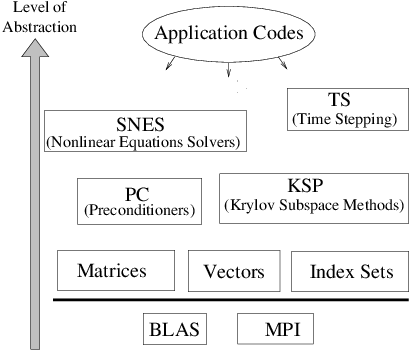
\includegraphics{petscwww}}
%\centerline{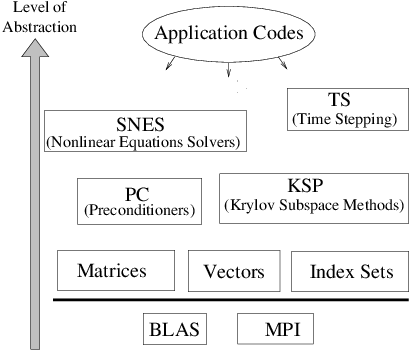
\psfig{file=petscwww.ps,angle=270,height=3.4in}}
% \centerline{\psfig{file=petsc_pt.eps,angle=0,height=4in,width=5in}}
\caption{Organization of the PETSc Libraries}
\label{fig_1}
\end{figure}

\begin{figure}[hbt]
\centerline{ 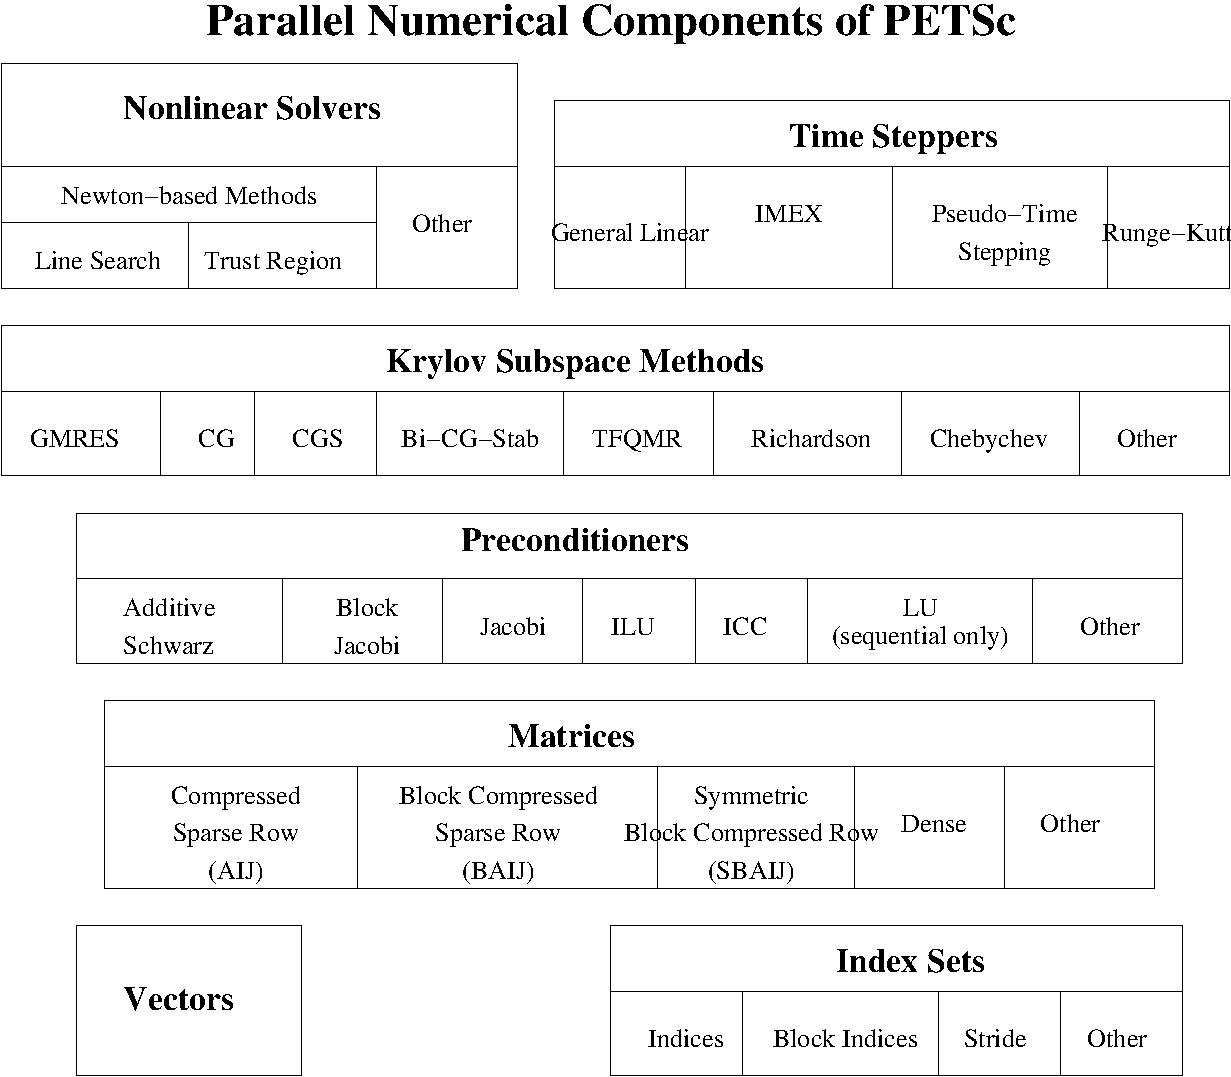
\includegraphics{zoom}}
%\centerline{\psfig{file=zoom_ls.ps,angle=270,height=3.4in}}
\caption{Numerical Libraries of PETSc}
\label{fig_2}
\end{figure}

\section{Suggested Reading}

The manual is
divided into three parts:
\begin{itemize}
\item Part I - Introduction to PETSc
\item Part II - Programming with PETSc
\item Part III - Additional Information
\end{itemize}

Part I describes
the basic procedure for using the PETSc library and presents two
simple examples of solving linear systems with PETSc.  This section
conveys the typical style used throughout the library and enables the
application programmer to begin using the software immediately.
Part I is also distributed separately for individuals interested in an 
overview of the PETSc software, excluding the details of library usage.
Readers of this separate distribution of Part I should note that all
references within the text to particular chapters and sections 
indicate locations in the complete users manual.

Part II explains in detail the use of the various PETSc libraries,
such as vectors, matrices, index sets, linear and nonlinear
solvers, and graphics.  Part III describes a variety of useful
information, including profiling, the options database, viewers, error
handling, makefiles, and some details of
PETSc design.

\nocite{efficient}

PETSc has evolved to become quite a comprehensive package, and therefore the
{\em PETSc Users Manual} can be rather intimidating for new users. We
recommend that one initially read the entire document before proceeding with
serious use of PETSc, but bear in mind that PETSc can be used efficiently
before one understands all of the material presented here. Furthermore, the
definitive reference for any PETSc function is always the online manualpage.

\medskip \medskip

Within the PETSc distribution, the directory \trl{${PETSC_DIR}/docs}
contains all documentation.
Manual pages for all PETSc functions can be
accessed on line at
\begin{tabbing}
  http://www.mcs.anl.gov/petsc/docs/
\end{tabbing}
The manual pages
provide hyperlinked indices (organized by
both concepts and routine names) to the tutorial examples and enable
easy movement among related topics.  

Emacs users may find the
{\em etags} option to be extremely useful for exploring the PETSc
source code.  Details of this feature are provided in
Section~\ref{sec_emacs}. 

The file \trl{manual.pdf} contains
the complete {\em PETSc Users Manual} in the portable document format (PDF), 
while \trl{intro.pdf} 
includes only the introductory segment, Part I.  \sindex{installing PETSc} 
The complete PETSc distribution, users
manual, manual pages, and additional information are also available via
the PETSc home page at
\trllink{http://www.mcs.anl.gov/petsc}{http://www.mcs.anl.gov/petsc}.  
The PETSc home page also
contains details regarding installation, new features and changes in recent
versions of PETSc, machines that we currently support, a
troubleshooting guide, and a FAQ list for frequently asked questions.

\medskip\medskip

\noindent{\bf Note to Fortran Programmers}: In most of the  
manual, the examples and calling sequences are given for the C/C++
family of programming languages.  We follow this convention because we
recommend that PETSc applications be coded in C or C++.
However, pure Fortran programmers can use most of the
functionality of PETSc from Fortran, with only minor differences in
the user interface.  Chapter \ref{ch_fortran} provides a discussion of the
differences between using PETSc from Fortran and C, as well as several
complete Fortran examples.  This chapter also introduces some
routines that support direct use of Fortran90 pointers.

%-----------------------------------------------------------------------------
\section{Running PETSc Programs}
\label{sec_running}

Before using PETSc, the user must first set the environmental variable
\trl{PETSC_DIR}, \findex{PETSC_DIR} indicating the full path of the PETSc home
directory.  For example, under the UNIX C shell a command of the form
\begin{tabbing}
   setenv PETSC\_DIR \$HOME/petsc
\end{tabbing}
 can be placed in the user's \trl{
.cshrc} file.  In addition, the user must set the environmental
variable {\trl{PETSC_ARCH}} to specify the architecture (e.g., rs6000,
solaris, IRIX, etc.)  on which PETSc is being used.  The utility
 \trl{${PETSC_DIR}/bin/petscarch} can be used for this purpose.  For example,
\begin{tabbing}
   setenv PETSC\_ARCH `\$PETSC\_DIR/bin/petscarch`
\end{tabbing}
can be placed in a \trl{.cshrc} file.  Thus, even if several machines of different
types share the same filesystem, \trl{PETSC_ARCH} will be set correctly
when logging into any of them. 

All PETSc programs use the MPI (Message Passing Interface) standard
for message-passing communication \cite{MPI-final}.  Thus, to execute
PETSc programs, users must know the procedure for beginning MPI jobs
on their selected computer system(s).  For instance, when using the
MPICH implementation of MPI \cite{mpich-web-page} and many others, the following
command initiates a program that uses eight processors:
\findex{mpirun} \sindex{running PETSc programs} 
\begin{tabbing}
   mpirun -np 8 petsc\_program\_name petsc\_options
\end{tabbing}

PETSc also comes with a script 
\begin{tabbing}
   \${PETSC\_DIR}/bin/petscmpirun -np 8 petsc\_program\_name petsc\_options
\end{tabbing}
that uses the information set in \trl{${PETSC_DIR}/bmake/${PETSC_ARCH}/packages} to 
automatically use the correct \trl{mpirun} for your configuration.

All PETSc-compliant programs support the use of the \trl{-h}
\findex{-h} or \trl{-help} option as well as the \trl{-v} \findex{-v}
or \trl{-version} option. 


Certain options are supported by all PETSc programs.  We list a few 
particularly useful ones below; a complete list can be obtained by 
running any PETSc program with the option \trl{-help}.
\begin{itemize}
\item \trl{-log_summary} - summarize the program's performance
\item \trl{-fp_trap} - stop on floating-point exceptions; \findex{-fp_trap}
      for example divide by zero
\item \trl{-trdump} - enable memory tracing; dump list of unfreed memory 
      at conclusion \findex{-trdump} of the run
\item \trl{-trmalloc} - enable memory tracing (by default this is 
      activated for versions of PETSc using BOPT=g*)
\item \trl{-start_in_debugger} \trl{[noxterm,gdb,dbx,xxgdb]} \trl{[-display name]} 
     - start all processes in debugger \findex{-start_in_debugger} \sindex{debugger}
\item \trl{-on_error_attach_debugger}  \trl{[noxterm,gdb,dbx,xxgdb]}
      \trl{[-display name]} - \findex{-on_error_attach_debugger}start debugger only on encountering an error
\end{itemize}
See Section \ref{sec_debugging} for more information on debugging PETSc programs.

%-----------------------------------------------------------------------------
\section{Writing PETSc Programs}
\label{sec_writing}

Most PETSc programs begin with a call to \findex{PetscInitialize()}
\begin{tabbing}
  PetscInitialize(int *argc,char ***argv,char *file,char *help);
\end{tabbing} 
which initializes PETSc and MPI.  The arguments \trl{argc} and 
\trl{argv} are the command line arguments delivered in all C and C++
programs. \sindex{command line arguments} The argument \trl{file}
optionally indicates an alternative name for the PETSc options file,
\trl{.petscrc}, which resides by default in the user's home directory.
Section \ref{sec_options} provides details regarding
this file and the PETSc options database, which can be used for runtime
customization. The final argument, \trl{help}, is an optional
character string that will be printed if the program is run with the
\trl{-help} option.  In Fortran the initialization command has the form
\begin{tabbing}
   call PetscInitialize(character(*) file,integer ierr)
\end{tabbing} 
\trl{PetscInitialize()} automatically calls \trl{MPI_Init()} if MPI
has not been not previously initialized. In certain \findex{MPI_Init()}
circumstances in which MPI needs to be initialized directly (or is
initialized by some other library), the user can first call 
\trl{MPI_Init()} (or have the other library do it), and then call
\trl{PetscInitialize()}.
By default, \trl{PetscInitialize()} sets the PETSc ``world''
communicator, given by \trl{PETSC_COMM_WORLD}, to \trl{MPI_COMM_WORLD}.
\findex{PETSC_COMM_WORLD}

For those not familar with MPI, a {\em communicator} is a way of
indicating a collection of processes that will be involved together
in a calculation or communication. Communicators have the variable type
\trl{MPI_Comm}. In most cases users can employ the communicator \trl{
PETSC_COMM_WORLD} to indicate all processes in a given run and \trl{
PETSC_COMM_SELF} to indicate a single process.
\findex{PETSC_COMM_SELF}

MPI provides routines
for generating new communicators consisting of subsets of processors,
though most users rarely need to use these. The book {\em Using MPI},
by Lusk, Gropp, and Skjellum \cite{using-mpi} provides an excellent
introduction to the concepts in MPI, see also the MPI homepage 
\trllink{http://www.mcs.anl.gov/mpi/}{http://www.mcs.anl.gov/mpi/}.
Note that PETSc users need not program much message passing directly
with MPI, but they must be familar with the basic concepts of message
passing and distributed memory computing.

All PETSc routines return an integer indicating whether an error has
occurred during the call.  The error code is set to be nonzero if an
error has been detected; otherwise, it is zero.  For the C/C++
interface, the error variable is the routine's return value, while for
the Fortran version, each PETSc routine has as its final argument an
integer error variable.  Error tracebacks are discussed in the following
section.

All PETSc programs should call \trl{PetscFinalize()} \findex{PetscFinalize()}
as their final (or nearly final) statement, as given below in the C/C++
and Fortran formats, respectively:
\begin{tabbing}
  PetscFinalize();\\
  call PetscFinalize(ierr)
\end{tabbing}
This routine handles options to be called at the conclusion of
the program, and calls \trl{MPI_Finalize()} \findex{MPI_Finalize()}
if \trl{PetscInitialize()}
began MPI. If MPI was initiated externally from PETSc (by either
the user or another software package), the user is
responsible for calling \trl{MPI_Finalize()}. 

\section{Simple PETSc Examples}

\label{sec_simple}

To help the user start using PETSc immediately, we begin with a simple
uniprocessor example in Figure~\ref{fig_example1} that solves the
one-dimensional Laplacian problem with finite differences.  This
sequential code, which can be found in 
\trl{${PETSC_DIR}/src/ksp/examples/tutorials/ex1.c},
illustrates the solution of a linear system with KSP, the 
interface to the preconditioners, Krylov subspace methods, and direct
linear solvers of PETSc.  Following the code we highlight a few of the most important
parts of this example.  

\begin{figure}[H]
{\footnotesize
\fileinclude{../../../src/ksp/examples/tutorials/ex1.c}
}
\caption{Example of Uniprocessor PETSc Code}
\label{fig_example1}
\end{figure}

\subsection*{Include Files}

The C/C++ include files for PETSc should be used via statements such as
\begin{tabbing}
{\footnotesize
   \#include "petscksp.h"
}
\end{tabbing}
where \trl{petscksp.h} is the include file for the linear solver library.
Each PETSc program must specify an
include file that corresponds to the highest level PETSc objects
needed within the program; all of the required lower level include
files are automatically included within the higher level files.  For
example, \trl{petscksp.h} includes \trl{petscmat.h} (matrices),
\trl{petscvec.h} (vectors), and \trl{petsc.h} (base PETSc file).  
The PETSc include files are located in the directory 
\trl{${PETSC_DIR}/include}.  See Section \ref{sec_fortran_includes}
for a discussion of PETSc include files in Fortran programs.

\subsection*{The Options Database}

As shown in Figure~\ref{fig_example1}, the user can input control data
at run time using the options database. In this example the command
\trl{PetscOptionsGetInt(PETSC_NULL,"-n",&n,&flg);} checks whether the user has
provided a command line option to set the value of \trl{n}, the
problem dimension.  If so, the variable \trl{n} is set accordingly;
otherwise, \trl{n} remains unchanged. A complete description of the
options database may be found in Section \ref{sec_options}.

\subsection*{Vectors}
\label{sec_vecintro}

One creates a new parallel or 
sequential vector, \trl{x}, of global dimension \trl{M} with the 
commands \findex{VecCreate()}  \findex{VecSetSizes()} \sindex{vectors}
\begin{tabbing}
  VecCreate(MPI\_Comm comm,Vec *x);
  VecSetSizes(Vec x, int m, int M);
\end{tabbing}
where \trl{comm} denotes the MPI communicator and \trl{m} is the optional local size
which may be \trl{PETSC_DECIDE}. The type of storage
for the vector may be set with either calls to 
\trl{VecSetType()} or \trl{VecSetFromOptions()}. \findex{VecSetType()} \findex{VecSetFromOptions()}
Additional vectors of the same type can be formed with
\findex{VecDuplicate()}
\begin{tabbing}
  VecDuplicate(Vec old,Vec *new);
\end{tabbing}
The commands \findex{VecSet()} \findex{VecSetValues()}
\begin{tabbing}
  VecSet(PetscScalar *value,Vec x);\\
  VecSetValues(Vec x,int n,int *indices,PetscScalar *values,INSERT\_VALUES);
\end{tabbing}
respectively set all the components of a vector to a particular scalar
value and assign a different value to each component.  More
detailed information about PETSc vectors, including their basic
operations, scattering/gathering, index sets, and distributed arrays, is
discussed in Chapter~\ref{chapter_vectors}.

\findex{PetscScalar} \sindex{complex numbers}
Note the use of the PETSc variable type \trl{PetscScalar} in this example.
The \trl{PetscScalar} is simply defined to be \trl{double} in C/C++
(or correspondingly \trl{double} \trl{precision} in Fortran) for versions of
PETSc that have {\em not} been compiled for use with complex numbers.
The \trl{PetscScalar} data type enables
identical code to be used when the PETSc libraries have been compiled
for use with complex numbers.  Section~\ref{sec_complex} discusses the
use of complex numbers in PETSc programs.

\subsection*{Matrices}
\label{sec_matintro}

Usage of PETSc matrices and vectors is similar. \sindex{matrices} 
The user can create a new parallel or sequential matrix, \trl{A}, which
has \trl{M} global rows and \trl{N} global columns, with the routine
\findex{MatCreate()}
\begin{tabbing}
  MatCreate(MPI\_Comm comm,int m,int n,int M,int N,Mat *A);
\end{tabbing}
where the matrix format can be specified at runtime.  The user could
alternatively specify each processes' number of local rows and columns
using \trl{m} and \trl{n}.
Values can then be set with the command
\begin{tabbing}
  MatSetValues(Mat A,int m,int *im,int n,int *in,PetscScalar *values,INSERT\_VALUES);
\end{tabbing}
After \findex{MatSetValues()} all elements have been inserted into the
matrix, it must be processed with the pair of commands
\findex{MatAssemblyBegin()} \findex{MatAssemblyEnd()}
\begin{tabbing}
  MatAssemblyBegin(Mat A,MAT\_FINAL\_ASSEMBLY);\\
  MatAssemblyEnd(Mat A,MAT\_FINAL\_ASSEMBLY);
\end{tabbing}
Chapter~\ref{chapter_matrices} discusses various matrix formats as
well as the details of some basic matrix manipulation routines.

\subsection*{Linear Solvers}

After creating the matrix and vectors that define a linear system,
\trl{Ax = b}, the user can then use KSP to solve the system 
with the following sequence of commands: 
\findex{KSPCreate()} \findex{KSPSetOperators()}
\findex{KSPSetFromOptions()} \findex{KSPSolve()} \findex{KSPDestroy()}
\begin{tabbing}
  KSPCreate(MPI\_Comm comm,KSP *ksp); \\
  KSPSetOperators(KSP ksp,Mat A,Mat PrecA,MatStructure flag);\\
  KSPSetFromOptions(KSP ksp);\\
  KSPSolve(KSP ksp,Vec b,Vec x);\\
  KSPDestroy(KSP ksp);
\end{tabbing}
The user first creates the KSP context and sets the operators
associated with the system (linear system matrix and optionally different
preconditioning matrix).  The user then sets various options for
customized solution, solves the linear system, and finally destroys
the KSP context.  We emphasize the command \trl{KSPSetFromOptions()}, 
which enables the user to customize the linear solution
method at runtime by using the options database, which is discussed in
Section~\ref{sec_options}. Through this database, the user not only
can select an iterative method and preconditioner, but also can prescribe
the convergence tolerance, set various monitoring routines, etc.
(see, e.g., Figure~\ref{fig_exprof}).

Chapter~\ref{ch_ksp} describes in detail the KSP package, including
the PC and KSP packages for preconditioners and Krylov subspace methods.

\subsection*{Nonlinear Solvers}
Most PDE problems of interest are inherently nonlinear. PETSc provides 
an interface to tackle the nonlinear problems directly called SNES. Chapter
\ref{chapter_snes} describes the nonlinear solvers in detail. We recommend 
most PETSc users work directly with SNES, rather than using PETSc
for the linear problem within a nonlinear solver.

\subsection*{Error Checking}

All PETSc routines return an integer indicating whether an error
has occurred during the call.  The PETSc macro \trl{CHKERRQ(ierr)}
checks the value of \trl{ierr} and calls the PETSc error handler
upon error detection.  \trl{CHKERRQ(ierr)} should be used in all
subroutines to enable a complete error traceback.
In Figure~\ref{fig_traceback} we indicate a
traceback generated by error detection within a sample PETSc
program. The error occurred on line 1673 of the file \trl{
${PETSC_DIR}/src/mat/impls/aij/seq/aij.c} and was caused by trying to allocate too
large an array in memory. The routine was called in the program 
\trl{ex3.c} on line 71.  See Section \ref{sec_fortran_errors} for
details regarding error checking when using the PETSc Fortran interface.

\begin{figure}[H]
\begin{tabbing}
   eagle:mpirun -np 1 ex3 -m 10000\\
   PETSC ERROR: MatCreateSeqAIJ() line 1673 in src/mat/impls/aij/seq/aij.c\\
   PETSC ERROR:   Out of memory. This could be due to allocating\\
   PETSC ERROR:   too large an object or bleeding by not properly\\
   PETSC ERROR:   destroying unneeded objects.\\
   PETSC ERROR:   Try running with -trdump for more information.\\ 
   PETSC ERROR: MatCreate() line 99 in src/mat/utils/gcreate.c  \\
   PETSC ERROR: main() line 71 in src/ksp/examples/tutorials/ex3.c\\  
   MPI Abort by user Aborting program !\\
   Aborting program! \\
   p0\_28969:  p4\_error: : 1
\end{tabbing}
\nobreak
\caption{Example of Error Traceback}
\label{fig_traceback}
\end{figure}

When running the debug (BOPT=g compiled) version of the PETSc libraries, it
does a great deal of checking for memory corruption (writing outside of 
array bounds etc). The macros \trl{CHKMEMQ} can be called 
anywhere in the code to check the current status of the memory for corruption.
By putting several (or many) of these macros into your code you can usually 
easily track down in what small segment of your code the corruption has occured.

\subsection*{Parallel Programming}

Since PETSc uses the message-passing model for
parallel programming and employs MPI for all interprocessor
communication, the user is free to employ MPI routines as needed
throughout an application code.  However, by default the user is
shielded from many of the details of message passing within PETSc,
since these are hidden within parallel objects, such as vectors,
matrices, and solvers.  In addition, PETSc provides tools such as
generalized vector scatters/gathers and distributed arrays to assist
in the management of parallel data.

\sindex{collective operations}
Recall that the user must specify a communicator upon creation of any
PETSc object (such as a vector, matrix, or solver) to indicate the
processors over which the object is to be distributed.  For example,
as mentioned above, some commands for matrix, vector, and linear solver
creation are:
\begin{tabbing}
  MatCreate(MPI\_Comm comm,int M,int N,Mat *A);\\
  VecCreate(MPI\_Comm comm,Vec *x);\\
  KSPCreate(MPI\_Comm comm,KSP *ksp); 
\end{tabbing}
The creation routines are collective over all processors in the
communicator; thus, all processors in the communicator {\em must}
call the creation routine.  In addition, if a sequence of
collective routines is being used, they {\em must} be called
in the same order on each processor.

The next example, given in Figure~\ref{fig_example2}, illustrates the
solution of a linear system in parallel.  This code, corresponding to
\trl{${PETSC_DIR}/src/ksp/examples/tutorials/ex2.c}, handles the
two-dimensional Laplacian discretized with finite differences, where
the linear system is again solved with KSP.  The code performs the
same tasks as the sequential version within Figure~\ref{fig_example1}.
Note that the user interface for initiating the program, creating
vectors and matrices, and solving the linear system is {\em exactly}
the same for the uniprocessor and multiprocessor examples.  The
primary difference between the examples in Figures \ref{fig_example1}
and \ref{fig_example2} is that each processor forms only its local
part of the matrix and vectors in the parallel case.

\begin{figure}[H]
{\footnotesize
\fileinclude{../../../src/ksp/examples/tutorials/ex2.c}
}
\nobreak
\caption{Example of Multiprocessor PETSc Code}
\label{fig_example2}
\end{figure}

\subsection*{Compiling and Running Programs}

Figure~\ref{fig_exrun} illustrates compiling and running a PETSc program
using MPICH.  Note that different sites may have slightly different
library and compiler names.  See Chapter \ref{ch_makefiles}
for a discussion about compiling PETSc programs.
Users who are experiencing difficulties linking PETSc programs should 
refer to the troubleshooting guide via the PETSc WWW home page 
\trllink{http://www.mcs.anl.gov/petsc}{http://www.mcs.anl.gov/petsc} or
given in the file \trllink{troubleshooting.html}{${PETSC_DIR}/docs/troubleshooting.html}.

\begin{figure}[H]
{\small
\begin{tabbing}
   eagle: make BOPT=g ex2\\
   gcc  -pipe -c  -I../../../  -I../../..//include   \\
       -I/usr/local/mpi/include  -I../../..//src -g \\
       -DPETSC\_USE\_DEBUG -DPETSC\_MALLOC -DPETSC\_USE\_LOG ex1.c\\
   gcc -g -DPETSC\_USE\_DEBUG -DPETSC\_MALLOC -DPETSC\_USE\_LOG -o ex1 ex1.o \\
      /home/bsmith/petsc/lib/libg/sun4/libpetscksp.a \\
      -L/home/bsmith/petsc/lib/libg/sun4 -lpetscstencil -lpetscgrid  -lpetscksp \\
      -lpetscmat  -lpetscvec -lpetscsys -lpetscdraw  \\
      /usr/local/lapack/lib/lapack.a /usr/local/lapack/lib/blas.a \\
      /usr/lang/SC1.0.1/libF77.a -lm /usr/lang/SC1.0.1/libm.a -lX11 \\
      /usr/local/mpi/lib/sun4/ch\_p4/libmpi.a\\
      /usr/lib/debug/malloc.o /usr/lib/debug/mallocmap.o  \\
      /usr/lang/SC1.0.1/libF77.a -lm /usr/lang/SC1.0.1/libm.a -lm\\
   rm -f ex1.o\\
   eagle: mpirun -np 1 ex2\\
   Norm of error 3.6618e-05 iterations 7\\
   eagle:\\
   eagle: mpirun -np 2 ex2\\
   Norm of error 5.34462e-05 iterations 9
\end{tabbing}
}
\nobreak
\caption{Running a PETSc Program}
\label{fig_exrun}
\end{figure}

As shown in Figure \ref{fig_exprof}, the option \trl{
-log_summary} activates printing of a performance summary, including
times, floating point operation (flop) rates, and message-passing
activity.  Chapter~\ref{ch_profiling}
provides details about profiling, including interpretation of the
output data within Figure~\ref{fig_exprof}.  This particular example involves the solution of a linear
system on one processor using GMRES and ILU.  The low floating point
operation (flop) rates in this example are due to the fact that the
code solved a tiny system.  We include this example merely to
demonstrate the ease of extracting performance information.

\begin{figure}[H]
{\footnotesize
\begin{verbatim}
eagle> mpirun -np 1 ex1 -n 1000 -pc_type ilu -ksp_type gmres -ksp_rtol 1.e-7 -log_summary
-------------------------------- PETSc Performance Summary: --------------------------------------

ex1 on a sun4 named merlin.mcs.anl.gov with 1 processor, by curfman Wed Aug  7 17:24:27 1996

                         Max         Min        Avg        Total 
Time (sec):           1.150e-01      1.0   1.150e-01
Objects:              1.900e+01      1.0   1.900e+01
Flops:                3.998e+04      1.0   3.998e+04  3.998e+04
Flops/sec:            3.475e+05      1.0              3.475e+05
MPI Messages:         0.000e+00      0.0   0.000e+00  0.000e+00
MPI Messages:         0.000e+00      0.0   0.000e+00  0.000e+00 (lengths)
MPI Reductions:       0.000e+00      0.0

--------------------------------------------------------------------------------------------------
Phase             Count      Time (sec)       Flops/sec                             -- Global --    
                            Max     Ratio    Max    Ratio   Mess  Avg len  Reduct  %T %F %M %L %R   
--------------------------------------------------------------------------------------------------
MatMult               2  2.553e-03    1.0  3.9e+06    1.0  0.0e+00 0.0e+00 0.0e+00  2 25  0  0  0
MatAssemblyBegin      1  2.193e-05    1.0  0.0e+00    0.0  0.0e+00 0.0e+00 0.0e+00  0  0  0  0  0
MatAssemblyEnd        1  5.004e-03    1.0  0.0e+00    0.0  0.0e+00 0.0e+00 0.0e+00  4  0  0  0  0
MatGetReordering      1  3.004e-03    1.0  0.0e+00    0.0  0.0e+00 0.0e+00 0.0e+00  3  0  0  0  0
MatILUFctrSymbol      1  5.719e-03    1.0  0.0e+00    0.0  0.0e+00 0.0e+00 0.0e+00  5  0  0  0  0
MatLUFactorNumer      1  1.092e-02    1.0  2.7e+05    1.0  0.0e+00 0.0e+00 0.0e+00  9  7  0  0  0
MatSolve              2  4.193e-03    1.0  2.4e+06    1.0  0.0e+00 0.0e+00 0.0e+00  4 25  0  0  0
MatSetValues       1000  2.461e-02    1.0  0.0e+00    0.0  0.0e+00 0.0e+00 0.0e+00 21  0  0  0  0
VecDot                1     60e-04    1.0  9.7e+06    1.0  0.0e+00 0.0e+00 0.0e+00  0  5  0  0  0
VecNorm               3  5.870e-04    1.0  1.0e+07    1.0  0.0e+00 0.0e+00 0.0e+00  1 15  0  0  0
VecScale              1  1.640e-04    1.0  6.1e+06    1.0  0.0e+00 0.0e+00 0.0e+00  0  3  0  0  0
VecCopy               1  3.101e-04    1.0  0.0e+00    0.0  0.0e+00 0.0e+00 0.0e+00  0  0  0  0  0
VecSet                3  5.029e-04    1.0  0.0e+00    0.0  0.0e+00 0.0e+00 0.0e+00  0  0  0  0  0
VecAXPY               3  8.690e-04    1.0  6.9e+06    1.0  0.0e+00 0.0e+00 0.0e+00  1 15  0  0  0
VecMAXPY              1  2.550e-04    1.0  7.8e+06    1.0  0.0e+00 0.0e+00 0.0e+00  0  5  0  0  0
KSPSolve             1  1.288e-02    1.0  2.2e+06    1.0  0.0e+00 0.0e+00 0.0e+00 11 70  0  0  0
KSPSetUp             1  2.669e-02    1.0  1.1e+05    1.0  0.0e+00 0.0e+00 0.0e+00 23  7  0  0  0
KSPGMRESOrthog        1  1.151e-03    1.0  3.5e+06    1.0  0.0e+00 0.0e+00 0.0e+00  1 10  0  0  0
PCSetUp               1 24e-02    1.0  1.5e+05    1.0  0.0e+00 0.0e+00 0.0e+00 18  7  0  0  0
PCApply               2  4.474e-03    1.0  2.2e+06    1.0  0.0e+00 0.0e+00 0.0e+00  4 25  0  0  0
-------------------------------------------------------------------------------------------------

Memory usage is given in bytes:

Object Type      Creations   Destructions   Memory  Descendants' Mem.
Index set             3              3      12420     0
Vector                8              8      65728     0
Matrix                2              2     184924     4140
Krylov Solver         1              1      16892     41080
Preconditioner        1              1          0     64872
KSP                  1              1          0     122844

\end{verbatim}
}
\nobreak
\caption{Running a PETSc Program with Profiling}
\label{fig_exprof}
\end{figure}

\subsection*{Writing Application Codes with PETSc}

The examples throughout the library demonstrate the software usage
and can serve as templates for developing
custom applications.  We suggest that new PETSc
users examine programs in the directories 
\begin{tabbing}
  \trl{${PETSC_DIR}/src/<library>/examples/tutorials},
\end{tabbing}
where \trl{<library>}
denotes any of the PETSc libraries (listed in the following
section), such as \trl{snes} or \trl{ksp}.  
The manual pages located at
\begin{tabbing}
   \${PETSC\_DIR}/docs/index.html or \\
   http://www.mcs.anl.gov/petsc/docs/
\end{tabbing}
provide indices (organized by both routine names and concepts) to the tutorial examples.

To write a new application program using PETSc, we suggest the
following procedure:
\begin{enumerate}
\item Install and test PETSc according to the instructions at the PETSc web site.
\item Copy one of the many PETSc examples in the directory
      that corresponds to the class of problem of interest (e.g.,
      for linear solvers, see \trl{${PETSC_DIR}/src/ksp/examples/tutorials}).
\item Copy the corresponding makefile within the example directory;
      compile and run the example program.
\item Use the example program as a starting point for developing a custom code.
\end{enumerate}

%---------------------------------------------------------------------

\section{Referencing PETSc}

When referencing PETSc in a publication please cite the following:
\begin{tabbing}
@Unpublished\{petsc-home-page,\\
   Author = "Satish Balay and William D. Gropp and Lois C. McInnes and Barry F. Smith",\\
   Title  = "PETSc home page",\\
   Note   = "http://www.mcs.anl.gov/petsc",\\
   Year   = "2001"\}\\

@TechReport\{petsc-manual,\\
   Author      = "Satish Balay and William D. Gropp and Lois C. McInnes and Barry F. Smith",\\
   Title       = "PETSc Users Manual",\\
   Number      = "ANL-95/11 - Revision 2.1.5",\\
   Institution = "Argonne National Laboratory",\\
   Year        = "2003"\}\\

@InProceedings\{petsc-efficient,\\
   Author    = "Satish Balay and William D. Gropp and Lois C. McInnes and Barry F. Smith",\\
   Title     = "Efficienct Management of Parallelism in Object Oriented Numerical Software Libraries",\\
   Booktitle = "Modern Software Tools in Scientific Computing",\\
   Editor    = "E. Arge and A. M. Bruaset and H. P. Langtangen",\\
   Pages     = "163--202",\\
   Publisher = "Birkhauser Press",\\
   Year      = "1997"\}
\end{tabbing}


%---------------------------------------------------------------------

\section{Directory Structure}

We conclude this introduction with an overview of the
organization of the PETSc software.  
The root directory of PETSc contains the following directories:
% As shown in Figure~\ref{fig_directories}, the root directory of PETSc contains the following directories:

\begin{itemize}
\item \trl{docs} - All documentation for PETSc. The files \trl{manual.pdf}
                   contains the hyperlinked users manual, suitable for printing
                   or on-screen viewering. Includes the subdirectory
 \subitem - \trl{manualpages} (on-line manual pages).
\item \trl{bin} - Utilities and short scripts for use with PETSc, including
 \begin{itemize}
 \item \trl{petsarch} (utility for setting \trl{PETSC_ARCH} environmental variable),
 \end{itemize}

\item \trl{bmake} - Base PETSc makefile directory.  Includes subdirectories
                    for various architectures.
\item \trl{include} - All include files for PETSc that are visible to the user.
\item \trl{include/finclude}    - PETSc include files for Fortran programmers using 
                                  the .F suffix (recommended).
\item \trl{include/pinclude}    - Private PETSc include files that should {\em not} 
                                  be used by application programmers.
\item \trl{src} - The source code for all PETSc libraries, which
                  currently includes
 \begin{itemize}
 \item \trl{vec} - vectors,
   \begin{itemize}
     \item \trl{is} - index sets,
   \end{itemize}
 \item \trl{mat} - matrices,
 \item \trl{dm}
   \begin{itemize}
    \item \trl{da} - distributed arrays,
    \item \trl{ao} - application orderings,
   \end{itemize}
 \item \trl{ksp} - complete linear equations solvers,
 \begin{itemize}
   \item \trl{ksp} - Krylov subspace accelerators,
   \item \trl{pc} - preconditioners,
 \end{itemize}
 \item \trl{snes} - nonlinear solvers
 \item \trl{ts} - ODE solvers and timestepping,
 \item \trl{sys} - general system-related routines,
 \begin{itemize}
   \item \trl{plog} - PETSc logging and profiling routines,
   \item \trl{draw} - simple graphics,
 \end{itemize}
 \item \trl{fortran} - Fortran interface stubs,
 \item \trl{contrib} - contributed modules that use PETSc but are not
    part of the official PETSc package.  We encourage users who have
    developed such code that they wish to share with others to let us
    know by writing to petsc-maint@mcs.anl.gov.
 \end{itemize}
\end{itemize}

Each PETSc source code library directory has the following subdirectories:
\begin{itemize}
\item  \trl{examples} - Example programs for the component, including
  \begin{itemize}
  \item \trl{tutorials} - Programs designed to teach users about PETSc.  These
          codes can serve as templates for the design of custom applicatinos.
  \item \trl{tests} - Programs designed for thorough testing of PETSc.  As such,
          these codes are not intended for examination by users.
  \end{itemize}
\item  \trl{interface} - The calling sequences for the abstract interface  
        to the component.
        Code here does not know about particular implementations.
\item  \trl{impls} - Source code for one or more implementations.
\item  \trl{utils} - Utility routines.  Source here may know about the 
          implementations, but ideally will not know about implementations
          for other components.
\end{itemize}

%
% Picture is not up to date, so temporarily exclude this.
%
% \begin{figure}[tb]
% \centerline{\psfig{file=dirs.ps,angle=270,height=6in,width=6in}}
% \nobreak
% \caption{Schematic of the PETSc Directory Structure}
% \label{fig_directories}
% \end{figure}


% ------------------------------------------------------------------
%   End of introductory information
% ------------------------------------------------------------------


% --------------------------------------------------------------------
%                            PART 2
% --------------------------------------------------------------------
\part{Programming with PETSc}
\label{part:usage}

\chapter{Vectors} 
\label{chapter:vectors}
\sindex{vectors}

PETSc provides two basic vector types: sequential and parallel
(MPI-based). To create a sequential vector with {\tt m} components,
one can
use the command \findex{VecCreateSeq()} \findex{Vec}
\begin{verbatim}
   ierr = VecCreateSeq(MPI_COMM_SELF,int m,Vec *x);
\end{verbatim}
To create parallel vectors one can either determine the number of 
components that will be stored on each processor or let PETSc decide. 
The command \findex{VecCreateMPI()}
\begin{verbatim}
   ierr = VecCreateMPI(MPI_Comm comm,int m,int M,Vec *x);
\end{verbatim}
creates parallel vectors. The argument {\tt m} indicates the number 
of components to store on the local processor, and {\tt M} is the 
total number of components in the vector.  Either of these two 
arguments, but not both, can be {\tt PETSC\_DECIDE} to 
\findex{PETSC_DECIDE} indicate that PETSc should determine the correct value. 
More generally, one should use the routine
\begin{verbatim}
  ierr = VecCreate(MPI_Comm comm,int M,Vec *v);
\end{verbatim}
which automatically selects the appropriate vector depending on the 
number of processors.

One can assign a single value to all components of a vector with the 
command \findex{VecSet()}
\begin{verbatim}
   ierr = VecSet(Scalar *value,Vec x);
\end{verbatim}
Assigning values to individual components of the vector is more 
complicated, in order to make it possible to write efficient parallel 
code.  Assigning a set of components is a two-step process: one 
first calls  \findex{VecSetValues()} \findex{INSERT_VALUES}
\begin{verbatim}
   ierr = VecSetValues(Vec x,int n,int *indices,Scalar *values,INSERT_VALUES);
\end{verbatim}
any number of times on any or all of the processors. The argument
{\tt n} gives the number of components being set in this 
insertion. The integer array {\tt indices} contains the global component
indices, and {\tt values} is the array of values to be inserted.
Any processor can set any components of the vector, PETSc insures that 
they are automatically stored in the correct location.
Once all of the values have been inserted, one must call \sindex{assembly}
\begin{verbatim}
   ierr = VecAssemblyBegin(Vec x);
\end{verbatim}
followed by \findex{VecAssemblyBegin()}\findex{VecAssemblyEnd()} 
\begin{verbatim}
   ierr = VecAssemblyEnd(Vec x);
\end{verbatim}
In order to allow the overlap of communication and calculation,
the user's code can perform any series of other actions between these 
two calls while the messages are in transition. 

\begin{design}
We have decided not to use an assembly context.  Although for repeated 
assemblies such a context
 may be a good idea, we wish to keep the design simple.
There are scatter contexts for gather-scatter operations, as discussed below.
\end{design}

Often, rather than inserting elements in a vector, one may wish to 
add values. This process \sindex{vector values, setting}
is also done with the command \findex{VecSetValues()}
\begin{verbatim}
   ierr = VecSetValues(Vec x, int n, int *indices, Scalar *values,ADD_VALUES);
\end{verbatim}
Again \findex{ADD_VALUES} one must call the assembly routines {\tt
VecAssemblyBegin()} and {\tt VecAssemblyEnd()} after all of the values
have been added.  Note that addition and insertion calls to {\tt
VecSetValues()} {\em cannot} be mixed.  Instead, one must add and insert
vector elements in phases, with intervening calls to the assembly
routines. This choice is to make implementations efficient, simple,
and more deterministic.

\begin{design}
Why have a single function, rather than an {\tt ADD\_VALUES} function and 
an {\tt INSERT\_VALUES} function?  This is to simplify the implementation 
codes, since otherwise there would be either code duplication or 
an additional subroutine call.
\end{design}

There is no routine called {\tt VecGetValues()}, since we provide 
an alternative method for selecting some components of a vector using
the vector scatters.  See Section \ref{sec:scatter} for details.

One can examine a vector with the command \findex{VecView()}
\begin{verbatim}
   ierr = VecView(Vec x,Viewer v);
\end{verbatim}
To print the vector to the screen, one uses the viewer
\findex{STDOUT_VIEWER_WORLD} {\tt STDOUT\_VIEWER\_WORLD}, which ensures
that parallel vectors are printed correctly to {\tt stdout}.  The
viewer {\tt STDOUT\_VIEWER\_SELF} \findex{STDOUT_VIEWER_SELF} can be employed if
the user does not care in what order the individual processors print
their pieces of the vector.  To display the vector in an X-window,
one uses either a {\tt DrawCtx} or {\tt DrawLGCtx} for the {\tt
Viewer} argument.  These drawing contexts are discussed in Section
\ref{sec:viewers}.

To create a new vector of the same format as an existing vector, one uses
the command \findex{VecDuplicate()}
\begin{verbatim}
   ierr = VecDuplicate(Vec old,Vec *new);
\end{verbatim}
To create several new vectors of the same format as an existing vector,
one uses the command \findex{VecGetVecs()}
\begin{verbatim}
   ierr = VecGetVecs(Vec old,int n,Vec **new);
\end{verbatim}
This routine creates an array of pointers to vectors. The two routines 
are very useful because they allow one to write library code that does 
not depend on the particular format of the vectors being used. Instead,
the subroutines can automatically correctly create work vectors
based on the specified existing vector.

When a vector is no longer needed, it should be destroyed with the 
command \findex{VecDestroy()}
\begin{verbatim}
   ierr = VecDestroy(Vec x);
\end{verbatim}
To destroy an array of vectors, one uses the command \findex{VecFreeVecs()}
\begin{verbatim}
   ierr = VecFreeVecs(Vec *vecs,int n);
\end{verbatim}

In certain circumstances it is desirable to use the sequential vectors
when running on one processor and the parallel vectors for two or
more.  The routine {\tt VecCreate()} \findex{VecCreate()}
automatically generates the appropriate vector type at runtime:
\begin{verbatim}
   ierr = VecCreate(MPI_Comm comm,int N,Vec *vec);
\end{verbatim}
Note that the option {\tt -vec\_mpi} can be used in conjunction with
{\tt VecCreate()} to specify the use of MPI vectors for the
uniprocessor case.

\section{Basic Vector Operations}
As listed in Figure \ref{fig:vectorops}, we have chosen certain 
basic vector operations to support within our vector library.
These operations were selected because they often arise in application 
codes, not because they have some inherent special properties. 

\begin{design}
Several of these operations could easily be constructed
by a combination of the other operations. 
We implement them directly to avoid a potentially large loss of efficiency, 
mainly because the vectors would have to go from main memory to the 
CPU two or more times, rather than just once.  Also, the arithmetic 
pipeline operations can be utilized more effectively.
\end{design}

\begin{figure}[H]
\centerline{
\begin{tabular}{ll}
{\bf Function Name} & {\bf Operation} \\
\hline
VecAXPY(Scalar *a,Vec x, Vec y); & $ y = y + a*x $ \\
VecAYPX(Scalar *a,Vec x, Vec y); & $ y = x + a*y $ \\
VecWAXPY(Scalar *a,Vec x,Vec y, Vec w); & $ w = a*x + y$ \\
VecScale(Scalar *a, Vec x); & $ x = a*x $\\
VecDot(Vec x, Vec y, Scalar *r); & $ r = \bar{x}'*y$\\
VecTDot(Vec x, Vec y, Scalar *r); & $ r = x'*y$\\
VecNorm(Vec x,  Scalar *r); & $ r = ||x||_{2}$\\
VecSum(Vec x,   Scalar *r); & $ r = \sum x_{i}$\\
VecCopy(Vec x, Vec y); & $ y = x $\\
VecSwap(Vec x, Vec y); & $ y = x $ while $ x = y$\\
VecPMult(Vec x,Vec y, Vec w); & $ w_{i} = x_{i}*y_{i} $ \\
VecPDiv(Vec x,Vec y, Vec w); & $ w_{i} = x_{i}/y_{i} $ \\
VecMDot(int n,Vec x, Vec *y,Scalar *r); & $ r[i] = \bar{x}'*y[i]$\\
VecMTDot(int n,Vec x, Vec *y,Scalar *r); & $ r[i] = x'*y[i]$\\
VecMAYPX(int n, Scalar *a,Vec x, Vec *y); \hspace{1cm} & 
                                    $ y[i] = x + a_{i}*y[i] $ \\
VecMax(Vec x,  int *idx, double *r); & $ r = \max x_{i}$\\
VecMin(Vec x,  int *idx, double *r); & $ r = \min x_{i}$\\
VecAbs(Vec x); & $ x_i = |x_{i}|$\\
VecReciprocal(Vec x); & $ x_i = 1/x_{i}$\\
VecShift(Scalar *s,Vec x); & $ x_i = s + x_{i}$\\
\hline 
\end{tabular}}
\label{fig:vectorops}
\caption{\hbox{PETSc Vector Operations}}
\end{figure}

For parallel vectors that are distributed across the processors by ranges, 
it is possible to determine \findex{VecGetOwnershipRange()}
a processor's local range with the routine
\begin{verbatim}
   ierr = VecGetOwnershipRange(Vec vec,int *low,int *high);
\end{verbatim}
This command is useful, for instance, in assembling matrices and 
right-hand-side vectors when using finite difference methods.
The argument {\tt low} indicates the first component owned by the local 
processor, while {\tt high} specifies {\bf one more}
than the last owned by the local processor.

\begin{design}
For vectors distributed in a general way across processors, we may need
the routine 
\begin{verbatim}
   ierr = VecGetOwnershipIndices(Vec, IS *is);
\end{verbatim}
This routine is not currently provided because our parallel vectors cannot
be laid out in this manner.
\end{design}

\section{Vector Internals}
On occasion the user needs to access the actual elements of the vector. 
The routine {\tt VecGetArray()} \findex{VecGetArray()}
returns a pointer to the elements local to the processor:
\begin{verbatim}
   ierr = VecGetArray(Vec v,Scalar **array);
\end{verbatim}
When access to the array is no longer needed, the user should call
\begin{verbatim}
   ierr = VecRestoreArray(Vec v, Scalar **array);
\end{verbatim}
The number of elements stored locally can be accessed with
\findex{VecGetLocalSize()}
\begin{verbatim}
   ierr = VecGetLocalSize(Vec v,int *size);
\end{verbatim}
The global vector length can be determined by \findex{VecGetSize()}
\begin{verbatim}
   ierr = VecGetSize(Vec v,int *size);
\end{verbatim}
 
\section{Index Sets} \sindex{index sets}
To facilitate general scatters and gathers, PETSc employs the 
concept of an index set.  An index set, which is a generalization of a 
set of integer indices, is used to define scatters, gathers, and similar 
operations on vectors and matrices. 

The following command creates a sequential index set based on a list 
of integers: \findex{ISCreateSeq()}
\begin{verbatim}
   ierr = ISCreateSeq(MPI_Comm comm,int n,int *indices, IS *is);
\end{verbatim}
This routine essentially copies the {\tt n} indices passed 
to it by the integer array {\tt indices}.  
Thus, the user should be sure to free the integer array {\tt indices} 
when it is no longer needed, perhaps directly after the call to 
{\tt ISCreateSeq}.

\begin{design}
This is an efficiency loss in the malloc needed for the 
index set and then the copy of the indices. But it seems to be the 
correct tradeoff in trying to maintain a ``clean'' and sensible interface.
One could perhaps provide an alternative interface, {\tt CreateFromUsersData},
but we have chosen not do that until we are certain that it is needed.
\end{design}

The second standard index set is defined by a starting point and a
stride. \sindex{stride}
The sequential \findex{ISCreateStrideSeq()} version can be created
with the command
\begin{verbatim}
   ierr = ISCreateStrideSeq(MPI_Comm comm,int n,int first,int step,IS *is);
\end{verbatim}

There is no parallel general index set. Instead, one creates a sequential
index set on each processor that needs one for the scatter-gather.

Index sets can be destroyed with the command, \findex{ISDestroy()}
\begin{verbatim}
   ierr = ISDestroy(IS is); 
\end{verbatim}

On rare occasions the user may have to access information directly 
from an index set. \findex{ISGetSize()} \findex{ISGetLocalSize()}
Several commands that \findex{ISStrideGetInfo()} \findex{ISGetIndices()}
assist in this process are
\begin{verbatim}
   ierr = ISGetSize(IS is, int *size);
   ierr = ISGetLocalSize(IS is, int *localsize);
\end{verbatim}
These both return the same value, because there is no need for a 
parallel index set distinct from a sequential one.
\begin{verbatim}
   ierr = ISStrideGetInfo(IS is, int *first,int *stride);
   ierr = ISGetIndices(IS is, int **indices);
\end{verbatim}
The function {\tt ISGetIndices()} returns a pointer to a list of the 
indices in the index set. 
For certain index sets, this may be a 
temporary array of indices created specifically for a given routine. 
Thus, once the user finishes using the array of indices, 
the routine \findex{ISRestoreIndices()}
\begin{verbatim}
   ierr = ISRestoreIndices(IS is, int **indices); 
\end{verbatim}
should be called to ensure that the system can free the space it 
used to generate the list of indices.

\begin{design}
One may reasonably ask why the scatter routines are based on 
using index sets while the vector assembly routines simply use 
arrays of integers. The reason for using index sets is to allow certain 
implementations to deal with strides and dense blocks of elements 
efficiently. In vector assembly, we are assuming that in the majority of 
cases the gain from using index sets is more than lost by requiring 
the users to build index sets for each insertion. 
\end{design}

\section{Scatters and Gathers} \sindex{scatter} \sindex{gather}
\label{sec:scatter}

PETSc vectors have full support for general scatters and 
gathers. One can select any subset of the components of a vector to
insert or add to any subset of the components of another vector.
We refer to these operations as generalized scatters, even though they are 
actually a combination of scatters and gathers. 

\begin{design}
It would be nice to have another word than scatter, but none is apparent.
\end{design}

To copy \findex{VecScatterCreate()} \findex{VecScatterBegin()}
components \findex{VecScatterEnd()} \findex{VecScatterDestroy()}
from one vector \findex{INSERT_VALUES} \findex{SCATTER_ALL}
to another use the set of commands,
\begin{verbatim}
   ierr = VecScatterCreate(Vec x,IS ix,Vec y,IS iy,VecScatter *ctx);
   ierr = VecScatterBegin(Vec x,Vec y,INSERT_VALUES,SCATTER_ALL,VecScatter ctx);
   ierr = VecScatterEnd(Vec x,Vec y,INSERT_VALUES,SCATTER_ALL,VecScatter ctx);
   ierr = VecScatterDestroy(VecScatter ctx);
\end{verbatim} 
Here {\tt ix} denotes the index set of the first vector, while {\tt iy} 
indicates the index set of the destination vector.
To add the values, rather than insert them, the user should select
 the option
{\tt ADD\_VALUES} \findex{ADD_VALUES} instead of {\tt INSERT\_VALUES}.

The vectors can be parallel or sequential.  The only 
requirements are that the number of entries in the index set of the
first vector, {\tt ix}, equals the number in the destination index set, 
{\tt iy}, and that the vectors are long enough to contain all the indices 
referred to in the index sets.
Note: Some of these combinations have not been coded yet.

To perform a gather operation, the user simply makes
 the destination index set, 
{\tt iy}, be a stride index set with a stride of one.  Similarly, a 
conventional scatter can be done with an initial (sending) index set 
consisting of a stride.  For parallel vectors, all processors that own 
the vector must call the scatter routines. When scattering from a 
parallel vector to sequential vectors, each processor has its own sequential 
vector that receives values from locations as indicated in its own 
index sets. Similarly, in scattering
from sequential vectors to a parallel vector, each processor has its
own sequential vector that makes contributions to the parallel vector.

Note:  If two different processors contribute different values to the 
same component in a parallel vector, either value may end up being 
inserted. When {\tt ADD\_VALUES} is used, the correct sum is added to the 
correct location.

\sindex{vector values, getting} \findex{VecGetValues() (pseudo)}
There is no PETSc routine that is the opposite of {\tt VecSetValues()}
\findex{VecSetValues()}.  Instead, the user creates a new vector where
the components are to be stored and creates the appropriate vector 
scatter. For example, if one desires to obtain the values for the 
100th and 200th entry from a parallel vector, {\tt p}, one could use 
a code such as the following:
\begin{verbatim}
  Vec        x;
  IS         from,to;
  int        idx_from[] = {100,200}, idx_to[] = {0,1};
  VecScatter scatter;
  Scalar     *values;
  ierr = VecCreateSeq(MPI_COMM_SELF,2,&x);
  ierr = ISCreateSeq(MPI_COMM_SELF,2,idx_from,&from);
  ierr = ISCreateSeq(MPI_COMM_SELF,2,idx_to,&to);
  ierr = VecScatterCreate(p,from,x,to,&scatter);
  ierr = VecScatterBegin(p,x,INSERT_VALUES,SCATTER_ALL,scatter);
  ierr = VecScatterEnd(p,x,INSERT_VALUES,SCATTER_ALL,scatter);
  ierr = VecGetArray(x,&values);
  ISDestroy(from); ISDestroy(to); VecScatterDestroy(scatter);
\end{verbatim}
The values for the 100th and 200th component now are in the array 
{\tt values}. In this example each processor now has the 100th and 
200th component, but obviously each processor could gather any 
elements it needed, or none by creating an index set with no entries.

The scatter is divided into two stages in order to allow overlap of 
communication and computation. The introduction of the 
{\tt ScatterCtx} allows the communication patterns for the scatter
to be computed once and then reused repeatedly. Generally, even 
setting up the communication for a scatter requires communication; 
hence, it is best to reuse that information when possible.

Two specialized routines \findex{VecPipelineBegin()} \sindex{pipeline}
are associated with the scatters: \findex{VecPipelineEnd()}
\begin{verbatim}
   VecPipelineBegin(Vec x,Vec y,INSERT_VALUES,PipelineMode mode,VecScatter ctx);
   VecPipelineEnd(Vec x,Vec y,INSERT_VALUES,PipelineMode mode,VecScatter ctx);
\end{verbatim}
These routines pipeline the scatter down through the processors (if 
{\tt mode} equals {\tt PIPELINE\_DOWN}) or up through the processors 
(if {\tt mode} equals {\tt PIPELINE\_UP}).
These routines are not commonly used.\findex{PIPELINE_DOWN}
\findex{PIPELINE_UP}

\begin{design}
The reason for these routines is to assist in coding Gauss-Seidel type 
algorithms. Since the communication patterns for 
Gauss-Seidel are the same as for the matrix-vector multiply, we wish
to reuse all of the setup code, as enabled by these functions.
\end{design}


% ------------------------------------------------------
\section{Distributed Arrays}

In this section we consider a distributed array to be not a matrix,
but a one-, two- or three-dimensional array of numbers distributed
across the processors, so that each processor contains a rectangular
subarray.  Distributed arrays are intended for use with regular,
rectangular grids when communication of nonlocal data is needed before
certain local computations can occur.  Distributed arrays are used in
conjunction with PETSc vectors.

For example, a typical situation one encounters in solving parallel
PDEs is that to evaluate a local function, {\tt f(x)}, each processor
requires its local portion of the vector {\tt x} as well as its ghost
points \sindex{ghost points} (the bordering portions of the vector
that are owned by neighboring processors).  Figure~\ref{fig:ghosts}
illustrates the ghost points for the seventh processor of a
two-dimensional, regular, parallel grid.  Each box represents a
processor; the ghost points for the seventh processor's local part of
a parallel array are shown in gray.

\begin{figure}[tb]
\centerline{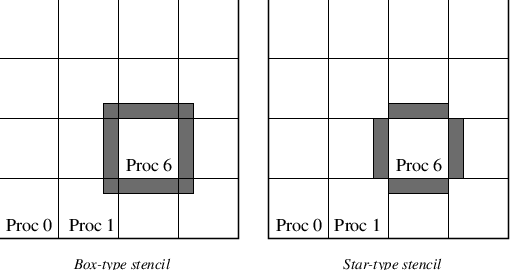
\psfig{file=papers/ghost.eps,angle=0}}
\caption{Ghost Points for two Stencil Types on the Seventh Processor}
\label{fig:ghosts}
\end{figure}

One creates a distributed array in two dimensions with the command 
\begin{verbatim}
  ierr = DACreate2d(MPI_Comm comm,DAPeriodicType wrap,DAStencilType st,int M,int N,
                    int m,int n,int dof,int s,DA *da);
\end{verbatim}
The \findex{DACreate2d} \sindex{array, distributed} arguments
\sindex{distributed array} {\tt M} and {\tt N} indicate the global
numbers of grid points in each direction, while {\tt m} and {\tt n}
denote the processor partition in each direction; {\tt m*n} must equal
the number of processors in {\tt comm}.  One may use instead 
{\tt PETSC\_DECIDE} and have PETSc determine the partition. The type of
periodicity of the array is specified by {\tt wrap}, which can be 
{\tt DA\_NONPERIODIC} \findex{DA_NONPERIODIC} (no periodicity), 
{\tt DA\_XYPERIODIC} \findex{DA_XYPERIODIC} (periodic in
both x- and y-directions), {\tt DA\_XPERIODIC} \findex{DA_XPERIODIC}, 
or {\tt DA\_YPERIODIC}.\findex{DA_YPERIODIC}  The argument {\tt dof} 
determines the number of degrees of freedom at each array point 
and {\tt s} is the stencil width.  

Two types of distributed arrays can be created, as specified by {\tt
st}.  Star-type stencils that radiate outward only in the coordinate
directions are indicated by {\tt DA\_STENCIL\_STAR}
\findex{DA_STENCIL_STAR}, while box-type stencils are specified by
{\tt DA\_STENCIL\_BOX} \findex{DA_STENCIL_BOX} For example, {\tt
DA\_STENCIL\_STAR} with width 1 corresponds to the standard 5-point
stencil, while {\tt DA\_STENCIL\_BOX} with width 1 denotes the
standard 9-point stencil.  In both cases the ghost points are
identical, the only difference being that with star-type stencils
certain ghost points are ignored, potentially decreasing substantially
the number of messages sent.  Note that the {\tt DA\_STENCIL\_STAR}
stencils can save interprocessor communication in two and three
dimensions.

The commands for creating distributed arrays in one and three
dimensions are analogous, as given by \findex{DACreate1d()}
\findex{DACreate3d()}
\begin{verbatim}
   ierr = DACreate1d(MPI_Comm comm,DAPeriodicType wrap,int M,int w,int s,DA *inra)
   ierr = DACreate3d(MPI_Comm comm,DAPeriodicType wrap,DAStencilType stencil_type,
                     int M,int N,int P,int m,int n,int p,int w,int s,DA *inra)
\end{verbatim}

The indices of the lower left corner of the local portion of the array 
as well as the local array size can be obtained with the commands
\findex{DAGetCorners()} \findex{DAGetGhostCorners()}
\begin{verbatim}
  ierr = DAGetCorners(DA da,int *x,int *y,int *z,int *m, int *n, int *p);
  ierr = DAGetGhostCorners(DA da,int *x,int *y,int *z,int *m, int *n, int *p);
\end{verbatim}
The first version excludes any ghost points, while the second version
includes them. Note that for interior subarrays the ghost corners can
easily be calculated from the true corners.  However, since the
calculation of ghost corners for boundary subarrays is not so
straightforward, both routines are provided.

Each {\tt DA} object contains two vectors: a distributed global vector, 
and a local vector that includes the appropriate ghost points. These
vectors can be accessed \findex{DAGetLocalVector()}
with the routines \findex{DAGetDistributedVector}
\begin{verbatim}
  ierr = DAGetDistributedVector(DA da,Vec *g);
  ierr = DAGetLocalVector(DA da, Vec *l);
\end{verbatim}
These two vectors will generally serve as the building blocks for 
local and global PDE solutions, etc.

At certain stages of many applications, there is a need to work 
on a local portion of the vector, including the ghost points. 
This may easily be done by scattering a global vector into its 
local parts by using the \findex{DAGlobalToLocalBegin()}
commands \findex{DAGlobalToLocalEnd()}
\begin{verbatim}
  ierr = DAGlobalToLocalBegin(DA da,Vec g, InsertMode iora, Vec l);
  ierr = DAGlobalToLocalEnd(DA da,Vec g, InsertMode iora, Vec l);
\end{verbatim}
Since the global and local vectors, given by {\tt g} and {\tt l} respectively,
must be compatible with the distributed array, {\tt da}, they should be
generated by {\tt DAGetDistributedVector()} 
\findex{DAGetDistributedVector()} and {\tt DAGetLocalVector()}
\findex{DAGetLocalVector()}
(or be duplicates of such vectors obtained via {\tt VecDuplicate()}).
The {\tt InsertMode} can be either {\tt ADD\_VALUES} or {\tt INSERT\_VALUES}.

The routine \findex{DAGetGhostCorners()} {\tt DAGetGhostCorners()}
deals with the fact that subarrays along boundaries of the problem
domain have ghost points only on their interior edges, but not on
their boundary edges.

One can scatter the local patches back into the distributed vector
with the command \findex{DALocalToGlobal()}
\begin{verbatim}
  ierr = DALocalToGlobal(DA da, Vec l, InsertMode mode, Vec g);
\end{verbatim}
Note that this function is not
subdivided into beginning and ending phases since it is purely local.

To assemble global stiffness matrices, one needs to be 
able to determine the global node number of each local node 
including the ghost nodes. This step may be done by using the 
command \findex{DAGetGlobalIndices()}
\begin{verbatim}
  ierr = DAGetGlobalIndices(DA da,int *n,int **idx);
\end{verbatim}
The output argument {\tt n} contains the number of 
local nodes, including ghost nodes, while {\tt idx} contains
a list of the global indices that correspond to the local nodes.

It is possible to directly access the vector scatter contexts 
used in the local-to-global ({\tt ltog}) and global-to-local 
({\tt gtol}) scatters with the command \findex{DAGetScatterCtx()}
\begin{verbatim}
  ierr = DAGetScatterCtx(DA da, VecScatter *ltog,VecScatter *gtol);
\end{verbatim}
Most users should not need to use these contexts.

When either type of stencil is used, {\tt DA\_STENCIL\_STAR} or 
{\tt DA\_STENCIL\_BOX}, the local vectors (with the ghost points) 
represent rectangular arrays, including the extra corner elements in 
the {\tt DA\_STENCIL\_STAR} case. This configuration provides simple 
access to the elements by employing 2- (or 3-) dimensional indexing. 
The only difference between the 
two cases is that when {\tt DA\_STENCIL\_STAR} is used, the extra 
corner components are not scattered between the processors.

Figure \ref{fig:daexample} illustrates the use 
of a distributed array in the solution of a nonlinear problem.
This is example {\tt \$(PETSC\_DIR)/src/snes/examples/ex6.c}.

\begin{figure}[H]
{\small
\fileinclude{../../src/snes/examples/ex6.c}
}
\caption{Use of Distributed Array}
\label{fig:daexample}
\end{figure}

%-------------------------------------------------------------
\chapter{Matrices}
\label{chapter:matrices}
\sindex{matrices}

PETSc 2.0 provides several standard matrix implementations.
Currently we support dense storage and compressed sparse row storage
(both sequential and parallel versions), as well as several 
specialized formats.  Additional formats can be added easily.
Matrix use involves the following actions: create a particular 
type of matrix, insert values into it, process the matrix, use the 
matrix for various computations, and finally destroy the matrix.
The application code does not need to know or care (and should not)
about the particular 
storage formats of the matrices.

\section{Basic Matrix Operations}
\label{sec:matoptions}

The first of the PETSc formats is the dense sequential matrix,
stored in a column major array in the usual Fortran 77 style. 
To create a dense, uniprocessor PETSc matrix the user should call
routine \findex{MatCreateSeqDense()}
\begin{verbatim}
   ierr = MatCreateSeqDense(MPI_COMM_SELF,int m, int n, Mat *A);
\end{verbatim}
The variables {\tt m} and {\tt n}, respectively, indicate the numbers
of rows and columns in the matrix, and {\tt A} is the new matrix.

The default sparse matrix representation supported in PETSc is the AIJ
\sindex{AIJ matrix format} format (also called the Yale sparse matrix
format or compressed row storage). By default the internal data
representation employs 0-based indexing.  For compatibility with
standard Fortran 77 storage, thus enabling use of external Fortran
software packages such as SPARSKIT, \sindex{SPARSKIT} the option {\tt
-mat\_aij\_oneindex} \findex{-mat_aij_oneindex} enables 1-based indexing, 
where the stored row and column indices begin at one, not zero.

To create a sequential AIJ sparse matrix \findex{MatCreateSeqAIJ()}
with {\tt m} rows and {\tt n} columns, use the command
\begin{verbatim}
   ierr = MatCreateSeqAIJ(MPI_COMM_SELF,int m,int n,int nz,int *nzz,Mat *A);
\end{verbatim}
The argument {\tt nz} indicates the expected number of nonzeros 
in each row. If one underestimates the actual value, then during the 
assembly process PETSc will automatically allocate additional needed space. 
However, since this extra memory allocation can slow the computation,
one may wish to to indicate the exact number of elements intended for
each row with the optional array, {\tt nzz}.  Thus, the assembly process 
will require no additional memory allocations that may slow it down. Again, if
the {\tt nnz} estimates are incorrect, then PETSc will automatically obtain
the additional needed space, at a slight loss of efficiency. 

Parallel sparse matrices with the AIJ 
format can be created with the command \findex{MatCreateMPIAIJ()}
\begin{verbatim}
   ierr = MatCreateMPIAIJ(MPI_Comm comm,int m,int n,int M,int N,int d_nz,
                          int *d_nnz, int o_nz,int *o_nnz,Mat *A);
\end{verbatim}
{\tt A} is the newly created matrix, while the arguments {\tt m}, {\tt n}, 
{\tt M}, and {\tt N}, respectively, indicate the number of local rows and 
columns and the number of global rows and columns. Either the local or
global parameters can be replaced with {\tt PETSC\_DECIDE}, so that 
PETSc will determine \findex{PETSC_DECIDE}
the correct value. The matrix is stored with a fixed number of rows on 
each processor, given by {\tt m}, or determined by PETSc if {\tt m} is
{\tt PETSC\_DECIDE}. 

The remaining arguments can simply be set to zero for PETSc to control
dynamic allocation of matrix memory space.  
Analogous to {\tt nz} and {\tt nnz} for the routine 
{\tt MatCreateSeqAIJ()}, these arguments optionally specify 
nonzero information for the diagonal ({\tt d\_nz} and {\tt d\_nnz}) and 
off-diagonal ({\tt o\_nz} and {\tt o\_nnz}) parts of the matrix. 
For a square global matrix we define each processor's diagonal portion 
to be its local rows and the corresponding columns (a square submatrix);  
each processor's off-diagonal portion encompasses the remainder of the
local matrix (a rectangular submatrix).  

The routine {\tt MatCreate()} \findex{MatCreate()} generates a
sequential matrix when running on one processor and a parallel matrix
for two or more processors, where the matrix format is determined from the
options database:
\begin{verbatim}
   int MatCreate(MPI_Comm comm,int M,int N,Mat *V)
\end{verbatim}
The user specifies only the global matrix dimensions, given by {\tt M}
and {\tt N}, while PETSc determines the appropriate local dimensions
and controls memory allocation.  By default, {\tt MatCreate()} employs
the sparse AIJ format.  This routine facilitates switching among
various matrix types, for example, to determine the format that is
most efficient for a particular application.   See
the man page for further information about available matrix formats.

The parallel matrix can multiply a vector with {\tt n} 
local entries, returning a vector with {\tt m} local entries. That is, 
to form the product \findex{MatMult()}
\begin{verbatim}
   ierr = MatMult(Mat A,Vec x,Vec y);
\end{verbatim}
the vectors {\tt x} and {\tt y} should be generated with 
\begin{verbatim}
   ierr = VecCreateMPI(n,N,&x);
   ierr = VecCreateMPI(m,M,&y);
\end{verbatim}
By default, if the user lets PETSc decide the number of components to
be stored locally, vectors and matrices of the same dimension are
automatically compatible for parallel matrix-vector operations.

To insert or add entries to a matrix (regardless of its particular format), 
one can call a variant of {\tt MatSetValues}, either \findex{MatSetValues()}
\begin{verbatim}
   ierr = MatSetValues(Mat A,int m,int *im,int n,int *in,Scalar *values,INSERT_VALUES);
\end{verbatim}
or 
\begin{verbatim}
   ierr = MatSetValues(Mat A,int m,int *im,int n,int *in,Scalar *values,ADD_VALUES);
\end{verbatim}
This routine inserts or adds a dense subblock of dimension {\tt m*n} to the 
matrix. The integer indices {\tt im} and {\tt in}, respectively, indicate the 
global rows and columns to be inserted.  {\tt MatSetValues()} uses the 
standard C convention, where the row and column matrix indices begin with 
zero {\em regardless of the storage format employed}.   The array 
{\tt values} is logically two-dimensional, containing the values that are 
to be inserted.   
By default the values are given in row major order, which is the opposite 
of the Fortran 77 convention. To allow the insertion of values in column 
major order, one can call the command \findex{MatSetOptions()}
\begin{verbatim}
   ierr = MatSetOption(Mat A,COLUMN_ORIENTED);
\end{verbatim}
Warning: Most of the sparse implementations do not currently support
the column-oriented option!

This notation should not be a mystery to anyone. For example, 
to insert one matrix into another when using Matlab, one uses the command 
{\tt A(im,in) = B;} where {\tt im} and {\tt in} contain the indices for the
rows and columns. This action is identical to the calls above to 
{\tt MatSetValues()}.

The function {\tt MatSetOption()} accepts several other inputs.  
We discuss two of these, which are related to the efficiency of the 
assembly process.  To indicate to PETSc that {\tt im} or {\tt in},
the indices inserted with {\tt MatSetValues()}, are sorted one uses  the 
commands \findex{ROWS_SORTED} \findex{COLUMNS_SORTED}
\begin{verbatim}
   ierr = MatSetOption(Mat A,ROWS_SORTED);
\end{verbatim}
and 
\begin{verbatim}
   ierr = MatSetOption(Mat A,COLUMNS_SORTED);
\end{verbatim}

After the matrix elements have been inserted or added into the matrix, 
it must be processed before it can be used. The routines for matrix
processing are \findex{MatAssemblyBegin()} \findex{MatAssemblyEnd()}
\begin{verbatim}
   ierr = MatAssemblyBegin(Mat A,FINAL_ASSEMBLY);
   ierr = MatAssemblyEnd(Mat A,FINAL_ASSEMBLY);
\end{verbatim}
Calls to {\tt MatSetValues()} with the {\tt INSERT\_VALUES} and {\tt
ADD\_VALUES} options {\em cannot} be mixed without intervening calls to
the assembly routines.  For such intermediate assembly calls the
second routine argument  typically should be {\tt FLUSH\_ASSEMBLY},
\findex{FLUSH_ASSEMBLY} which omits some of the work of the full 
asembly process.  {\tt FINAL\_ASSEMBLY} \findex{FINAL_ASSEMBLY} is
required only in the last matrix assembly before a matrix is used.

Even though one may insert values into PETSc matrices without regard
to which processor the values are eventually stored on, for efficiency
reasons it is usually recommended to generate most entries on the
processor where they are destined to be stored.  To help the
application programmer with this task for matrices that are
distributed across the processors by ranges, the routine
\findex{MatGetOwnershipRange()}
\begin{verbatim}
   ierr = MatGetOwnershipRange(Mat A,int *first_row,int *last_row);
\end{verbatim}
informs the user that all rows from {\tt first\_row} to 
{\tt last\_row-1} will be stored on the local processor.

In the sparse matrix implementations, once the assembly routines have been 
called, the matrices are compressed and can be used for matrix-vector
multiplication, etc.
Inserting new values into the matrix at this point will be expensive, 
since it requires copies and possible memory allocation. Thus, whenever 
possible one should completely set the values in the matrices before 
calling the final assembly routines. 

Along with the matrix-vector multiplication routine given above, there is 
a version for the transpose of the matrix, \findex{MatMultTrans()}
\begin{verbatim}
   ierr = MatMultTrans(Mat A,Vec x,Vec y);
\end{verbatim}
There are also versions that add the result
to another vector, \findex{MatMultAdd()} \findex{MatMultTransAdd()}
\begin{verbatim}
   ierr = MatMultAdd(Mat A,Vec x,Vec y,Vec w);
   ierr = MatMultTransAdd(Mat A,Vec x,Vec y,Vec w);
\end{verbatim}
These routines respectively produce $w = A*x + y$ and $w = A^{T}*x + y$. 
In C it is legal for the vectors {\tt y} and {\tt w} to be identical.
In Fortran 77, this situation is forbidden by the language standard, 
but it may be useful at times regardless.

\begin{design}
Instead of four routines, why not have
one routine with an extra argument to indicate the details? That is 
the approach in LAPACK and seems a natural extension of the 
{\tt SetValues()} routines. One difference is that the {\tt Add} 
routines take one additional argument.
\end{design}

One can print a matrix (sequential or parallel) to the screen with the 
command \findex{MatView()}
\begin{verbatim}
   ierr = MatView(Mat mat, STDOUT_VIEWER_WORLD);
\end{verbatim}
Other viewers can be used as well. For instance, one can draw the matrix
in an X-window with the command
\begin{verbatim}
   ierr = MatView(Mat mat,(Viewer) DrawCtx win);
\end{verbatim}
See Section \ref{sec:viewers} for additional viewers and options.


\section{Matrix-Free Matrices} \sindex{matrix-free methods}

\label{sec:matrixfree}
Some people like to use matrix-free methods, which do not require
explicit storage of the matrix, for the numerical solution of partial 
differential equations.  
To support matrix-free methods in PETSc, one can create a 
{\tt Mat} structure without ever actually generating the matrix.  
This is achieved with the command \findex{MatShellCreate()}
\begin{verbatim}
   ierr = MatShellCreate(MPI_Comm comm,int m, int n, void *ctx, Mat *mat);
\end{verbatim}
Most matrix-free algorithms require only the application of 
the linear operator to a vector. To provide this action, the user must 
write a routine with the calling sequence
\begin{verbatim}
   ierr = Mult(void *ctx,Vec x,Vec y);
\end{verbatim}
and then associate it with the matrix, {\tt mat}, by using the 
command \findex{MatShellSetMult()}
\begin{verbatim}
   ierr = MatShellSetMult(Mat mat, int (*mult)(void* ctx,Vec,Vec));
\end{verbatim}
Now this matrix can be used with the iterative linear equation solvers 
discussed in the following chapters.
Other routines include \findex{MatShellSetMultTransAdd()}
\begin{verbatim}
   ierr = MatShellSetMultTransAdd(Mat mat, int (*mult)(void* ctx,Vec,Vec,Vec));
\end{verbatim}

\section{Other Matrix Operations}
\label{sec:othermat}.

In many iterative calculations, for instance in a nonlinear equations
solver, it is important for efficiency purposes to reuse the nonzero 
structure of a matrix, rather than determining it anew every time 
the matrix is generated.  To retain a given matrix but reinitialize
its contents, one can employ \findex{MatZeroEntries()}
\begin{verbatim}
   ierr = MatZeroEntries(Mat A);
\end{verbatim}
For sparse matrices this routine will zero the matrix entries in the 
data structure but keep all the data that indicates where the nonzeros
are located.  In this way a new matrix assembly will be much less 
expensive since no memory allocations or copies will be needed. 
By default, if new entries are made in locations where no nonzeros 
previously existed, space will be allocated for the new entries. 
To prevent the allocation of additional memory and simply discard those 
new entries, one can use the option \findex{MatSetOptions()}
\begin{verbatim}
   ierr = MatSetOption(Mat A,NO_NEW_NONZERO_LOCATIONS);
\end{verbatim}
Once the matrix has been assembled, one can factor it numerically
without repeating the ordering or the symbolic factorization. 
This option can save some computational time, although it
does require that the factorization is not done in-place.

In the numerical solution of elliptic partial differential equations,
it can be cumbersome to deal with Dirichlet boundary 
\sindex{boundary conditions} conditions. In
particular, one would like to assemble the matrix without regard to 
boundary conditions and then at the end apply the Dirichlet boundary 
conditions. 
In numerical analysis classes this process is usually presented as moving the 
known boundary conditions to the right hand side and then solving a smaller
linear system for the interior unknowns. Unfortunately, implementing this
requires extracting a large submatrix from the original matrix and 
creating its corresponding data structures. This process can be expensive 
in both time and memory. 

One simple way to deal with this difficulty is to replace those rows in the 
matrix associated with known boundary conditions, by rows of the 
identity matrix (or some scaling of it). This action can be done with 
the command \findex{MatZeroRows()}
\begin{verbatim}
   ierr = MatZeroRows(Mat A, IS rows, Scalar *diagonal_value);
\end{verbatim}
For sparse matrices this removes the data structures for certain rows 
of the matrix. If the pointer {\tt diagonal\_value} is zero, it 
even removes the diagonal entry. If the pointer is nonzero, it uses that 
given value in the diagonal entry of the eliminated rows. 

One nice feature of this approach is that when solving a nonlinear problem 
such that at each iteration the Dirichlet boundary conditions are in the 
same positions and the matrix retains the same nonzero structure, the user 
can call {\tt MatZeroRows} in the first iteration. Then, before generating 
the matrix in the second iteration the user should call
\begin{verbatim}
   ierr = MatSetOption(Mat A,NO_NEW_NONZERO_LOCATIONS);
\end{verbatim}
From that point, \findex{MatSetOptions()}
no new values will be inserted into those rows of 
the matrix. \findex{NO_NEW_NONZERO_LOCATIONS} 

Another matrix routine of interest is \findex{MatConvert()}
\begin{verbatim}
   ierr = MatConvert(Mat mat,MatType newtype,Mat *M)
\end{verbatim}
which converts the matrix {\tt mat} to new matrix, {\tt M}, that has
either the same or different format.  Set {\tt newtype} to {\tt MATSAME}
to copy the matrix, keeping the same matrix format.  See 
{\tt \$(PETSC\_DIR)/include/mat.h} for other available matrix types.

In certain applications it may be necessary for application codes
to access directly elements of a matrix. This may be done by using the 
the command 
\begin{verbatim}
  ierr = MatGetRow(Mat A,int row, int *ncols,int **cols,Scalar **vals);
\end{verbatim}
The argument {\tt ncols} returns the number of nonzeros in that row, 
while {\tt cols} and {\tt vals} returns the column indices (with indices
starting at zero) and values in the row. If one only needs the column 
indices and not the values, one may pass in a 0 for the {\tt vals}
argument. Similarly one may pass a 0 in for the {\tt cols} argument.
The user can only examine these values, they cannot be changed. 
To change \findex{MatGetRow()} \findex{MatRestoreRow()}
them, one must use {\tt MatSetValues()}.

Once you have finished with that row, you {\bf must} call 
\begin{verbatim}
  ierr = MatRestoreRow((Mat A,int row, int *ncols,int **cols,Scalar **vals);
\end{verbatim}
This frees any space that was allocated during the call to 
{\tt MatGetRow()} and resets any data items that may have been 
changed. The reason for the {\tt MatRestoreRow()} command is that 
most of the sparse matrix storage formats are not simply by rows. 
Thus the {\tt MatGetRow()} must allocate some space before presenting 
it to the user.
 

\section{Matrix Factorization} \sindex{factorization}
\label{sec:matfactor}

Most application programmers will not directly use the matrix
factorization and matrix solve routines, but instead will access them
indirectly through the SLES interface, (see Chapter \ref{sec:sles},
which provides easy and portable access to both direct and iterative
solvers).  We therefore suggest that most users can skip this section.

\begin{design}
Factorization is tricky because we would like to allow a lot
of flexibility in terms of ordering, symbolic factorization 
reuse, in-place factorization etc., while still maintaining a
small set of functions. 
\end{design}

The LU and Cholesky \sindex{Cholesky}
matrix factorizations are split into \sindex{LU}
two or three stages depending on the user's needs. The first stage is 
to calculate an ordering for the matrix.  The ordering generally is 
done to reduce fill in a sparse factorization; it does not make much 
sense for a dense matrix. \findex{MatGetReordering()} \sindex{reorder}
\begin{verbatim}
   ierr = MatGetReordering(Mat matrix,MatOrdering type,IS* rowperm,IS* colperm); 
\end{verbatim}
The currently available alternatives for the ordering {\tt type} are 
\begin{itemize}
\item {\tt ORDER\_NATURAL} - Natural
\item {\tt ORDER\_ND} - Nested Dissection
\item {\tt ORDER\_1WD} - One-way Dissection
\item {\tt ORDER\_RCM} - Reverse Cuthill-McGee
\item {\tt ORDER\_QMD} - Quotient Minimum Degree
\end{itemize}
These orderings can also be set through the options database by specifying 
one of the following:  {\tt -mat\_order natural, -mat\_order nd, 
-mat\_order 1wd, -mat\_order rcm, -mat\_order qmd}.
Certain \findex{ORDER_NATURAL} \findex{ORDER_ND} \findex{ORDER_1WD}
matrix \findex{ORDER_RCM} \findex{ORDER_QMD} \sindex{nested dissection}
\sindex{one-way dissection} \sindex{reverse Cuthill-McGee} 
\sindex{quotient minimum degree} \findex{-mat_order}
formats may support only a subset of these. More options may 
be added in the future; check the manual pages. All of these orderings are 
symmetric at the moment. In the future, ordering routines that are 
not symmetric may be added.

The next routines do complete, in-place, symbolic and numerical 
factorizations for symmetric and nonsymmetric matrices, respectively:
\begin{verbatim}
   ierr = MatCholeskyFactor(Mat matrix,IS permutation,double pf);
   ierr = MatLUFactor(Mat matrix,IS rowpermutation, IS columnpermutation, double pf); 
\end{verbatim}
The argument {\tt pf $ \ge $ 1} is the predicted fill
expected in the factored matrix, as a ratio of the original fill. 
For example, {\tt 2.0} would indicate that one expects the factored
matrix to have twice as many nonzeros as the original.
\findex{MatCholeskyFactor()} \findex{MatLUFactor()}

\begin{design}
For sparse matrices it is very unlikely that the factorization 
is actually done ``in-place''. More likely, new space is allocated 
for the factored matrix and the old space deallocated, but to the 
user it is ``in-place'' because the unfactored matrix gets replaced with 
the factored matrix.
\end{design}

The \sindex{symbolic factorization}
two \findex{MatCholeskyFactorSymbolic()} \findex{MatLUFactorSymbolic()}
stages \findex{MatCholeskyFactorNumeric()} \findex{MatLUFactorNumeric()}
can also be done separately, in the out-of-place mode:
\begin{verbatim}
   ierr = MatCholeskyFactorSymbolic(Mat matrix,IS perm, double pf,Mat *result);
   ierr = MatLUFactorSymbolic(Mat matrix,IS rowperm, IS colperm,double pf,Mat *result);
   ierr = MatCholeskyFactorNumeric(Mat matrix, Mat *result);
   ierr = MatLUFactorNumeric(Mat matrix, Mat *result);
\end{verbatim}
In this case, the contents of the matrix {\tt result} is undefined between 
the symbolic and numeric factorization stages. 
It is possible to reuse the symbolic factorization. For the second and 
succeeding factorizations, one simply calls the numerical factorization with a 
new input {\tt matrix} and the {\em same} factored {\tt result} matrix
(the numerical factorization merely overwrites the numerical values in the 
factored matrix and does not disturb the symbolic portion which is why 
it may be reused).
It is VITAL that the new input matrix have the 
exact same nonzero structure as the original factored matrix.
In general, calling {\tt XXXFactorSymbolic} with a dense matrix will 
do nothing except allocate the new matrix; the {\tt XXXFactorNumeric} 
routines will do all of the work. 

\begin{design}
Why have the plain {\tt XXXfactor} routines when one could simply 
call the two stage routines? The answer is that if one desires an in-place 
factorization of a sparse matrix, the intermediate stage between the 
symbolic and numeric phases cannot be stored in a {\tt result} matrix and
it doesn't really make sense to store the intermediate valuses
 inside the original matrix 
that is being transformed.  We originally made the combined factor routines
do either an in-place or out-of-place factorization, but then decided that 
this approach was not needed and could easily lead to confusion.
\end{design}

We do not presently support sparse matrix factorization with pivoting 
for numerical stability. This is because that can get complicated, 
trying to both reduce fill and do privoting. Instead, we provide a 
poor step-child substitute. After one has obtained a reordering one may 
call,
\begin{verbatim}
ierr = MatReorderForNonzeroDiagonal(Mat A,double tol,IS row, IS col);
\end{verbatim}
This will try to reorder the columns to insure that no values along 
the diagonal are smaller then {\tt tol} in a absolute value. If small 
values are detected and corrected for, this will result in a nonsymmetric
permutation of the rows and columns. This is not guaranteed to work, 
but may help if you were simply unlucky in your original ordering.

\begin{design}
The second argument to {\tt XXXNumeric} is a {\tt Mat*} 
rather than a {\tt Mat}, to be consistent with  certain other functions.
\end{design}

Once a matrix has been factored, it is natural to solve linear systems.
The following four routines enable this: \findex{MatSolve()} 
\begin{verbatim}
   ierr = MatSolve(Mat A,Vec x, Vec y);
   ierr = MatSolveTrans(Mat A, Vec x, Vec y);
   ierr = MatSolveAdd(Mat A,Vec x, Vec y, Vec w);
   ierr = MatSolveTransAdd(Mat A, Vec x, Vec y, Vec w);
\end{verbatim}
The \findex{MatSolveTrans()} \findex{MatSolveAdd()}
matrix \findex{MatSolveTransAdd()}
{\tt A} of these routines must have been obtained from a 
factorization routine; otherwise, an error will be generated.
In general, the user should use the SLES solvers introduced in the 
next chapter rather then using these factorization and solve routines
directly.

\begin{design}
Again, should we have four routines or one, with an extra argument?
\end{design}

% ------------------------------------------------------------------
\chapter{SLES: Linear Equations Solvers} \sindex{linear system solvers}
\label{sec:sles}

SLES is the heart of PETSc, since it provides uniform and efficient access 
to all of the package's linear system solvers, both parallel and sequential,
direct and iterative.
SLES is intended for solving systems of the form
\begin{equation}
   A x = b,
\label{eq:Ax=b}
\end{equation}
where $A$ denotes the matrix representation of a linear operator, $b$
is the right-hand-side vector, and $x$ is the solution vector.  SLES
uses the same calling sequence for both direct and iterative solution
of a linear system.  In addition, particular solution techniques and
their associated options can be selected at runtime.

The combination of a Krylov space method and a preconditioner is at
the center of most modern numerical codes for the iterative solution of
linear systems.  See, for example, \cite{fgn} for an overview of the theory
of such methods.  SLES creates a simplified interface to the
lower-level KSP and PC modules within the PETSc package.  The KSP component, 
discussed in
Section~\ref{sec:ksp}, provides many popular Krylov
\sindex{Krylov subspace iterative methods} subspace iterative methods;
the PC module, described in Section~\ref{sec:pc}, includes a
variety of preconditioners.  Although both  KSP and PC can be used
directly, most users should employ the interface of SLES.

\section{Using SLES} 
\label{sec:usingsles}

To solve a linear system with SLES, one must first create a solver context 
with the command \findex{SLESCreate()}
\begin{verbatim}
   ierr = SLESCreate(MPI_Comm comm,SLES *sles); 
\end{verbatim}
Here {\tt comm} is the MPI communicator and {\tt sles} is the newly
formed solver context.
Before actually solving a linear system with SLES, the user must call 
the following routine to set the matrices associated with the linear
system: \findex{SLESSetOperators()}
\begin{verbatim}
   ierr = SLESSetOperators(SLES sles, Mat Amat,Mat Pmat,MatStructure flag);
\end{verbatim}
The argument {\tt Amat}, representing the matrix that defines the
linear system, is a symbolic place holder for any kind of matrix.  
In particular, note that SLES {\bf does} support matrix-free methods. 
See \sindex{matrix-free methods}
the routine {\tt MatShellCreate()} \findex{MatShellCreate()}
in Section~\ref{sec:matrixfree} for further information regarding
matrix-free methods. 
Typically the preconditioning matrix, {\tt Pmat}, is the same as
the matrix that defines the linear system, {\tt Amat}; however,
occasionally these matrices differ (for instance, \sindex{preconditioning}
when preconditioning a matrix obtained from a high order method with 
that from a low order method).

The argument {\tt flag} can be used to eliminate unnecessary work when
repeatedly solving linear systems of the same size with the same 
preconditioner.  The user can set {\tt flag} to be
{\tt MAT\_SAME\_NONZERO\_PATTERN}, {\tt PMAT\_SAME\_NONZERO\_PATERN},
or {\tt ALLMAT\_SAME\_NONZERO\_PATERN} to indicate, respectively, that 
the linear sysem matrix, preconditioning matrix, or both have the same 
\findex{MAT_SAME_NONZERO_PATTERN} \findex{PMAT_SAME_NONZERO_PATTERN} 
\findex{ALLMAT_SAME_NONZERO_PATTERN} 
nonzero structure as during of the previous solve. If {\tt pmat} is zero,
this indicates that the previous preconditioner should be reused.
 
Much of the power of SLES can be accessed through the single routine
\begin{verbatim}
   ierr = SLESSetFromOptions(SLES sles);
\end{verbatim}
This \findex{SLESSetFromOptions()}
routine accepts the options {\tt -h} and {\tt -help} as well as 
any of the KSP and PC options discussed below. 
To solve a linear system, merely execute the command \findex{SLESSolve()}
\begin{verbatim}
   ierr = SLESSolve(SLES sles, Vec b, Vec x, int *its);
\end{verbatim}
Here {\tt b} denotes the right-hand-side vector, {\tt x} indicates
the solution vector, and {\tt its} is the number of iterations 
required for convergence.
Note that multiple linear solves can be performed by the same SLES context.
Once the SLES context is no longer needed, it should be destroyed with the 
command \findex{SLESDestroy()}
\begin{verbatim}
   ierr = SLESDestroy(SLES sles);
\end{verbatim}

The above procedure is sufficient for general use of the SLES package.
One additional step is required for users who wish to customize certain 
preconditioners (e.g., see Section~\ref{sec:bjacobi}) or to log certain 
performance data using the PETSc profiling facilities (as discussed in 
Chapter~\ref{ch:profiling}).
In this case, the user can optionally explicitly call \findex{SLESSetUp()}
\begin{verbatim}
   ierr = SLESSetUp(SLES sles,Vec b,Vec x);
\end{verbatim}
before calling {\tt SLESSolve()} to perform any setup required for 
the linear solvers.  The explicit call of this routine enables the
separate monitoring of any computations performed during the set up
phase, such as incomplete factorization for the ILU preconditioner.

To allow application programmers to set any of the preconditioner or 
Krylov subspace options directly within the code, we provide routines
that extract the PC and KSP contexts, \findex{SLESGetPC()}
\begin{verbatim}
   ierr = SLESGetPC(SLES sles, PC *pc);
\end{verbatim}
and \findex{SLESGetKSP()}
\begin{verbatim}
   ierr = SLESGetKSP(SLES sles, KSP *ksp);
\end{verbatim}
The application programmer can then directly call any of the PC or KSP 
routines to modify the corresponding default options. 

To solve a linear system with a direct solver (presently supported 
only for sequential matrices) one may use the options, 
{\tt -pc\_method lu} with {\tt -ksp\_method preonly}, (see below).

\begin{design}
In order for SLES to be the trivially simple preconditioner plus
a Krylov method, we have decided that one of the preconditioners will be 
direct factorization. The default SLES can be direct preconditioner 
plus ``apply preconditioner'' for the  Krylov space method.
 This may be forcing
a square block into a round hole, but we think it is worth doing. 
Old SLES became overly complicated and complex; we will force new
SLES to be simple by decreasing the concepts with which it must deal.
\end{design}

\begin{design}
By default, if a direct solver is used, the factorization is NOT done 
in-place. This approach, is to prevent the user from the unexpected surprise
of having a corrupted matrix after a linear solve. The routine 
{\tt PCLUSetUseInPlace()}, discussed below, causes factorization to 
be done in-place. \findex{PCLUSetUseInPlace()} 
\end{design}


\section{KSP Component}\sindex{Krylov subspace methods}
\label{sec:ksp}

The Krylov space methods accept a large number of options, many of which 
are discussed below.  First, to set the Krylov space method that is to 
be used, one calls the command \findex{KSPSetMethod()}
\begin{verbatim}
   ierr = KSPSetMethod(KSP ksp,KSPMethod method);
\end{verbatim}
The method can be one of {\tt KSPRICHARDSON, KSPCHEBYCHEV, KSPCG, KSPGMRES, 
KSPTCQMR, KSPBCGS, KSPCGS, KSPTFQMR, KSPCR, KSPLSQR}, or {\tt KSPPREONLY.}
\findex{KSPRICHARDSON} \findex{KSPCHEBYCHEV} \findex{KSPCG}
\findex{KSPGMRES} \findex{KSPTCQMR} \findex{KSPBCGS} \findex{KSPTFQMR}
\findex{KSPCR} \findex{KSPPREONLY}
The KSP method can also be set with the options database command 
{\tt -ksp\_method},
followed by one of the options {\tt richardson, chebychev, cg, gmres, tcqmr, 
bcgs, cgs, tfqmr, cr, lsqr}, or {\tt preonly.} \findex{-ksp_method}
There are method-specific options for the Richardson, Chebychev,
and GMRES \findex{KSPChebychevSetEigenvalues()} \findex{KSPGMRESSetRestart()}
methods: \findex{KSPRichardsonSetScale()}  \sindex{GMRES} \sindex{CG}
\begin{verbatim}
   ierr = KSPRichardsonSetScale(KSP ksp,double damping_factor);
   ierr = KSPChebychevSetEigenvalues(KSP ksp,double emax,double emin);
   ierr = KSPGMRESSetRestart(KSP ksp,int max_steps);
\end{verbatim}
The default parameter values are {\tt damping\_factor=1.0, 
emax=0.01, emin=100.0}, and {\tt max\_steps=10.0}. The GMRES 
\sindex{restart} restart
can also be set from the options database with {\tt -ksp\_gmres\_restart n}.
\findex{-ksp_gmres_restart}

By default, the GMRES solver uses a modified Gram-Schmidt method 
during the orthogonalization process. A fast approach is to use the 
unmodified Gram-Schmidt method, which can be done \sindex{Gram-Schmidt}
with \findex{KSPGMRESSetUseUnmodifiedGramSchmidt()} 
\begin{verbatim}
   ierr = KSPGMRESSetUseUnmodifiedGramSchmidt(KSP ksp);
\end{verbatim}
or the options database command {\tt -ksp\_gmres\_unmodifiedgramschmidt}.
Note that this algorithm is numerically unstable, but may deliver 
much better speed performance.

By default, KSP assumes an initial guess of zero by zeroing the initial 
value for the solution vector that is given. To use a nonzero 
initial guess, the user {\em must} call \findex{KSPSetInitialGuessNonzero()}
\begin{verbatim}
   ierr = KSPSetInitialGuessNonzero(KSP ksp);
\end{verbatim}

\subsection{Preconditioning within KSP} 
\label{sec:ksppc}
\sindex{preconditioning}

Since the rate of convergence of Krylov projection methods for a
particular linear system is strongly dependent on its spectrum,
preconditioning is typically used to alter the spectrum and hence
accelerate the convergence rate of iterative techniques.
Preconditioning can be applied to the system (\ref{eq:Ax=b}) by
\begin{equation}
   (M_L^{-1} A M_R^{-1}) \, (M_R x) = M_L^{-1} b,
\label{eq:prec}
\end{equation}
where $M_L$ and $M_R$ indicate preconditioning matrices.  If $M_L = I$
in (\ref{eq:prec}), right preconditioning results, and the
residual of (\ref{eq:Ax=b}),
  \[ r \equiv b - Ax = b - A M_R^{-1} \, M_R x, \]
is preserved.  In contrast, the residual is altered for left 
($M_R = I$) and symmetric preconditioning, as given by
  \[ r_L \equiv M_L^{-1} b - M_L^{-1} A x = M_L^{-1} r. \]
By default, all KSP implementations use left preconditioning.  
Right preconditioning can be activated for some methods by
using the options database command {\tt -ksp\_right\_pc} or
calling the routine \findex{-ksp_right_pc}
\begin{verbatim}
   ierr = KSPSetRightPreconditioner(KSP ksp);
\end{verbatim}

We summarize the defaults for the residuals used in KSP convergence
monitoring within Table~\ref{tab:kspdefaults}.  Details regarding
specific convergence tests and monitoring routines are presented in
the following sections.  The preconditioned residual is used by
default for convergence testing of all left-preconditioned KSP
methods {\em except} for the conjugate gradient, Richardson, and
Chebyshev methods.  For these three cases the true residual is used by
default, but the preconditioned residual can be employed instead with
the options database command {\tt ksp\_preres} or by calling the routine
\begin{verbatim}
   ierr = KSPSetUsePreconditionedResidual(KSP ksp);
\end{verbatim}

\begin{table}
\caption{KSP Defaults.  All methods use left preconditioning by default.}
\begin{center}
\begin{tabular}{lll}
{\bf KSP Method}	& {\bf Options Database Name}	& {\bf Default Convergence Monitor}\\
\hline
KSPRICHARDSON	& richardson	& true residual	 \\
KSPCHEBYCHEV	& chebychev	& true residual	\\
KSPCG		& cg		& true residual	 \\
KSPGMRES	& gmres		& preconditioned residual \\
KSPTCQMR	& tcqmr		& preconditioned residual \\
KSPBCGS		& bcgs		& preconditioned residual \\
KSPCGS		& cgs		& preconditioned residual \\
KSPTFQMR	& tfqmr		& preconditioned residual \\
KSPCR		& cr		& preconditioned residual \\
KSPLSQR		& lsqr		& preconditioned residual \\
KSPPREONLY	& preonly	& preconditioned residual \\
\hline
\end{tabular}
\end{center}
\label{tab:kspdefaults}
\end{table}

\subsection{Convergence}

The default convergence test, {\tt KSPDefaultConverged()}, is 
based on the discrete $L_2$-norm of the residual. Convergence 
(or divergence) is decided by three quantities:
the relative decrease of the residual norm, {\tt rtol}, the absolute 
size of the residual norm, {\tt atol}, and the relative increase in the 
residual, {\tt dtol}.  Convergence is detected at iteration $k$ if
\[  \| r_k \|_2 < {\rm max} ( rtol * \| r_0 \|_2, atol ), \]
where $r_k = b - A x_k$.  Divergence is detected if
\[  \| r_k \| > dtol * \| r_0 \|. \]
These parameters, as well as the maximum number of allowable iterations, 
can be set with the routine \findex{KSPSetTolerances()}
\begin{verbatim}
   ierr = KSPSetTolerances(KSP ksp,double rtol,double atol,double dtol,int maxits);
\end{verbatim}
The user can retain the default value of any of these parameters by
specifying {\tt PETSC\_DEFAULT} \findex{PETSC_DEFAULT} as the 
corresponding tolerance; the
defaults are {\tt rtol}=$10^{-5}$, {\tt atol}=$10^{-50}$, and {\tt
dtol}=$10^{5}$, and {\tt maxits}=$10^5$.
These parameters can also be set from the options database with the 
commands {\tt -ksp\_rtol rtol, -ksp\_atol atol}, {\tt -ksp\_divtol dtol},
\findex{-ksp_rtol} \findex{-ksp_atol} \findex{-ksp_divtol}
and {\tt -ksp\_max\_it its}. \findex{-ksp_max_it}

In addition to providing an interface to a simple convergence test,
KSP allows the application programmer the flexibility to provide 
customized convergence testing routines.  \sindex{convergence tests}
The application programmer can provide a customized convergence test 
routine with the command \findex{KSPSetConvergenceTest()}
\begin{verbatim}
   KSPSetConvergenceTest(KSP ksp,int (*test)(KSP ksp,int it,double rnorm,void *ctx),
                         void *ctx);
\end{verbatim}
The final routine argument, {\tt ctx}, is an optional context for private
data for the user-defined convergence routine, {\tt test}.  Other
{\tt test} routine arguments are the iteration
number ({\tt it}) and the residual's $L_2$ norm ({\tt rnorm}).
The convergence test {\tt test}, should return the 
integer 1 for convergence, 0 for no convergence, and -1 on error or 
failure to converge.  
 
\subsection{Monitoring Convergence}

By default, the Krylov solvers run silently without displaying information 
about the iterations. The user can indicate that the norms of the residuals 
should be displayed by using \findex{-ksp_monitor}
{\tt -ksp\_monitor} within the options database.  
To display the residual norms in a graphical window (running under X Windows),
one should use {\tt -ksp\_xmonitor [x,y,w,h]}, where either all or none of 
the options must be specified. \findex{-ksp_xmonitor}
Application programmers can also provide their own routines to perform 
the monitoring by using the command \findex{KSPSetMonitor()}
\begin{verbatim}
   KSPSetMonitor(KSP ksp,int (*mon)(KSP ksp, int it, double rnorm, void *ctx),void *ctx);
\end{verbatim}
The final routine argument, {\tt ctx}, is an optional context for private
data for the user-defined monitoring routine, {\tt mon}.  Other
{\tt mon} routine arguments are the iteration
number ({\tt it}) and the residual's $L_2$ norm ({\tt rnorm}).
A helpful routine within user-defined monitors is 
{\tt PetscObjectGetComm((PetscObject)ksp,MPI\_Comm *comm)}, which returns
in {\tt comm} \findex{PetscObjectGetComm()} \sindex{communicator} the
MPI communicator for the {\tt KSP} context.  See Chapter~\ref{chapter:design}
for more discussion of the use of MPI communicators within PETSc.

Several default monitoring routines are supplied with PETSc, 
including \findex{KSPDefaultMonitor()} \findex{KSPDefaultCGMonitor()}
\begin{verbatim}
   KSPDefaultMonitor(KSP,int,double, void *);
   KSPDefaultCGMonitor(KSP,int,double, void *);
\end{verbatim}
The default monitor simply prints an estimate of the $L_2$-norm of the 
residual at each iteration. The routine
{\tt KSPDefaultCGMonitor} is appropriate only for use with the conjugate 
gradient method, as it prints estimates of the extreme eigenvalues of the 
preconditioned operator at each iteration.

To employ the default graphical monitor, one should use the 
commands \findex{KSPLGMonitorCreate()} \findex{KSPLGMonitorDestroy()}
\begin{verbatim}
   DrawLGCtx lg;
   ierr = KSPLGMonitorCreate(char *display,char *title,int x,int y,int w,int h,DrawLGCtx *lg);
   ierr = KSPSetMonitor(KSP ksp,KSPLGMonitor,(void *)lg);
\end{verbatim}
When no longer needed, the line graph should be destroyed 
with the command
\begin{verbatim}
   ierr = KSPLGMonitorDestroy(DrawLGCtx lg);
\end{verbatim}
The user can change aspects of the graphs with the {\tt DrawLG*()} and 
{\tt DrawAxis*()} routines. \findex{DrawAxis*()} \findex{DrawLG*()}

\begin{design}
The reason that merely calling {\tt DrawLGDestroy()} is insufficient is
that the underlying window structure must be destroyed as well.
\end{design}

\subsection{Other KSP Options}

To obtain the solution vector and right hand side from a KSP 
context, one uses \findex{KSPGetSolution()} \findex{KSPGetRhs()}
\begin{verbatim}
   ierr = KSPGetSolution(KSP ksp,Vec *x);
   ierr = KSPGetRhs(KSP ksp,Vec *rhs);
\end{verbatim}
These routines return the original vectors that the user set with 
{\tt KSPSetSolution()} and {\tt KSPSetRhs()}. \findex{KSPSetSolution()}
During \findex{KSPSetRhs()} the iterative process
the solution may not yet have been calculated or it may be stored in 
a different location. To access the approximate solution during the 
iterative process, one uses, the command \findex{KSPBuildSolution()}
\begin{verbatim}
   ierr = KSPBuildSolution(KSP ksp,Vec w,Vec *v);
\end{verbatim}
where the solution is returned in {\tt v}. The user can optionally provide
a vector in {\tt w} as the location to store the vector; however, if 
{\tt w} is 0, space is allocated by PETSc in the KSP context is 
used. One should not destroy this vector. For certain KSP methods, 
(e.g. GMRES), the construction of the solution is expensive, while for many 
others it requires not even a vector copy. 

Access to the residual is done in a similar way with the 
command \findex{KSPBuildResidual()}
\begin{verbatim}
   ierr = KSPBuildResidual(KSP ksp, Vec t,Vec w, Vec *v);
\end{verbatim}
Again, for GMRES and certain other methods this is an expensive 
operation.

\subsection{Unimportant Details of KSP}

Again, virtually all users should use KSP through the SLES interface, 
and thus will not need to know the details that follow. 

It is possible to generate a Krylov space context with the 
command \findex{KSPCreate()}
\begin{verbatim}
   ierr = KSPCreate(MPI_Comm comm,KSP *kps);
\end{verbatim}
Before using the Krylov context, the matrix-vector multiplication routine and
the preconditioner must be set with the 
commands \findex{PCSetOperators()} \findex{KSPSetBinv()}
\begin{verbatim}
   ierr = PCSetOperators(PC pc,Mat mat,Mat pmat,MatStructure flag);
   ierr = KSPSetBinv(KSP ksp,PC pc);
\end{verbatim}
In addition, the KSP solver must be initialized with \findex{KSPSetUp()}
\begin{verbatim}
   ierr = KSPSetUp(KSP ksp);
\end{verbatim}
Solving a linear system is done with the command \findex{KSPSolve()}
\begin{verbatim}
   ierr = KSPSolve(KSP ksp,int *its);
\end{verbatim}
Finally, the KSP context should be destroyed with \findex{KSPDestroy()}
\begin{verbatim}
   ierr = KSPDestroy(KSP ksp);
\end{verbatim}

\begin{design} 
It may seem strange to put the matrix in the preconditioner rather
than directly in the KSP; this decision was the result of much
agonizing. The reason is that for SSOR with Eisenstat's trick, and 
certain other preconditioners, the
preconditioner has to change the matrix-vector multiply.  This 
procedure could not
be done cleanly if the matrix were stashed in the KSP context that
PC cannot access.
\end{design}

\begin{design}
We have added a new feature to KSP. Any preconditioner can supply not 
only the preconditioner, but also a routine that essentially performs a
complete Richardson step. The reason for this is mainly SOR. To 
use SOR in the Richardson framework, that is 
\[
  u^{n+1} = u^{n} + B(f - A u^{n}), 
\]
is much more expensive than just updating the values.
With this addition it is reasonable to state that ALL our
iterative methods are obtained by combining a preconditioner from 
the {\tt PC} component with a Krylov method from the {\tt KSP}
component. This strategy makes things much simpler conceptually, so 
(we hope)
clean code will result. NOTE: We had this idea already implicitly in 
older versions of SLES, but, for instance, just doing Gauss-Seidel
with Richardson in old SLES is much more expensive than it had to be. 
With PETSc 2.0 this should not be a problem. 
\end{design}

We have made sure that all the Krylov space codes compile for the 
complex version. We do NOT claim that they are coded correctly 
for complex numbers; almost surely, most, if not all, are incorrect. 
Mostly they would be incorrect due to the use of the wrong inner 
product, since for complex numbers the inner product is not 
symmetric. This error should be fixed someday!

\section{Preconditioners} \sindex{preconditioners}
\label{sec:pc}

As discussed in Section~\ref{sec:ksppc}, the Krylov space methods are
typically used in conjunction with a preconditioner.
To employ a particular preconditioning method, the user can either select 
it from the options database using input of the form 
{\tt -pc\_method methodname}, or set the method with the 
command \findex{PCSetMethod()} \findex{-pc_method}
\begin{verbatim}
   ierr = PCSetMethod(PC pc,PCMethod method);
\end{verbatim}
The most basic methods are {\tt PCNONE, PCJACOBI, PCBJACOBI,
PCSOR, PCESOR, PCICC, PCILU, 
PCLU}, and {\tt PCSHELL}. \findex{PCNONE} \findex{PCJACOBI} \findex{PCSOR}
\findex{PCICC} \findex{PCLU} \findex{PCILU} \findex{PCSHELL} 
The \findex{PCBJACOBI} corresponding string names for use with the options 
database are {\tt none, jacobi, bjacobi, sor, eisenstat, icc, ilu, lu}, 
and {\tt shell}, respectively. The {\tt PCSHELL} preconditioner uses a 
specific, application-provided preconditioner. 
The direct preconditioner is, in fact, a direct solver for the linear system 
that uses LU or Cholesky factorization. It is included as a preconditioner 
so that PETSc has a consistent interface among direct and iterative 
linear solvers.

Each preconditioner may have associated with it a set of options,
which can be set with routines and options database commands provided
for this purpose.  Such routine names and commands are all of the form
{\tt PC<METHOD>Option} and {\tt pc\_<method>\_option [value]}.  A
complete list can be found by consulting the manual pages; we discuss
few in the sections below.

\subsection{SOR and SSOR Preconditioners}

The options for SOR \sindex{SSOR} \sindex{SOR} \sindex{relaxation}
preconditioning are \findex{PCSORSetOmega()}
\begin{verbatim}
   ierr = PCSORSetOmega(PC pc,double omega);
   ierr = PCSORSetIterations(PC pc,int its);
   ierr = PCSORSetSymmetric(PC pc,MatSORType type);
\end{verbatim}
The \findex{PCSORSetIterations()} \findex{PCSORSetSymmetric()}
first of these commands sets the relaxation factor for successive
over (under) relaxation.  The second command sets the number of inner
iterations of SOR, given by {\tt its}, to use between steps of the
Krylov space method.  The third command sets the kind of SOR sweep,
where the argument {\tt type} can be one of {\tt SOR\_FORWARD\_SWEEP,
SOR\_BACKWARD\_SWEEP} or {\tt SOR\_SYMMETRIC\_SWEEP}, the default
being {\tt SOR\_FORWARD\_SWEEP}. Setting the type to be {\tt
SOR\_SYMMETRIC\_SWEEP} produces the SSOR method.  In addition, 
each processor can locally and independently perform the specified 
variant of SOR with the types {\tt SOR\_LOCAL\_FORWARD\_SWEEP, 
SOR\_LOCAL\_BACKWARD\_SWEEP}, and {\tt SOR\_LOCAL\_SYMMETRIC\_SWEEP}.
These \findex{SOR_FORWARD_SWEEP} \findex{SOR_BACKWARD_SWEEP}
variants \findex{SOR_SYMMETRIC_SWEEP} \findex{SOR_LOCAL_FORWARD_SWEEP}
can \findex{SOR_LOCAL_BACKWARD_SWEEP} \findex{SOR_LOCAL_SYMMETRIC_SWEEP}
also be set with the \findex{-pc_sor_omega} \findex{-pc_sor_its}
\findex{-pc_sor_backward} \findex{-pc_sor_symmetric}
\findex{-pc_sor_local_forward} \findex{-pc_sor_local_backward}
\findex{-pc_sor_local_symmetric} options {\tt -pc\_sor\_omega omega}, 
{\tt -pc\_sor\_its its}, {\tt -pc\_sor\_backward}, {\tt -pc\_sor\_symmetric}, 
{\tt -pc\_sor\_local\_forward}, {\tt -pc\_sor\_local\_backward}, and 
{\tt -pc\_sor\_local\_symmetric}, respectively.

The Eisenstat trick \sindex{Eisenstat trick} for SSOR preconditioning 
can be employed with the method PCESOR \findex{PCEISENSTAT} 
({\tt -pc\_method eisenstat}).  
By using both left and right preconditioning of the linear system,
this variant of SSOR requires about half of the floating point operations 
for conventional SSOR.  {\tt PCEisenstatUseDiagonalScaling()} (or the
option {\tt -pc\_eisenstat\_diagonal\_scaling}) 
\findex{-pc_eisenstat_diagonal_scaling} 
\findex{PCEisenstatUseDiagonalScaling()} activates diagonal
scaling in conjunction with Eisenstat SSOR method, while
{\tt PCEisenstatSetOmega(PC pc, double omega)} 
\findex{PCEisenstatSetOmega()} (or the 
option {\tt -pc\_eisenstat\_omega omega}) \findex{-pc_eisenstat_omega omega}
sets the SSOR relaxation coefficient, {\tt omega}, as discussed above.

\findex{PCEisenstatUseDiagonalScaling()}

\subsection{LU Factorization}

The LU preconditioner provides two options.  The first, given by
the \sindex{direct solver}
command \findex{PCLUSetUseInPlace()} \findex{inplace solvers}
\begin{verbatim}
   ierr = PCLUSetUseInPlace(PC pc);
\end{verbatim}
causes the factorization to be performed in-place, and hence
obviously destroys the original matrix.  The options database variant of
this command is {\tt -pc\_lu\_in\_place}. \findex{-pc_lu_in_place}
Another direct preconditioner option is selecting the ordering
of equations with the command \findex{-mat_order}
\begin{verbatim}
   -mat_order ordering
\end{verbatim}
The possible orderings are the same as those used by the routine 
{\tt MatGetReordering()}, \findex{MatGetReordering()}
discussed in Section~\ref{sec:matfactor}.


\subsection{Block Jacobi Preconditioner}
\label{sec:bjacobi}

At present, the block Jacobi method \sindex{Jacobi} \sindex{block Jacobi} 
may be the best choice for parallel preconditioning.  
By default, the block Jacobi methods employs LU factorization on each
individual block; the user can set alternative linear solvers via the options 
\findex{-sub_ksp_method} \findex{-sub_pc_method}
{\tt -sub\_ksp\_method} and {\tt -sub\_pc\_method}. In fact, all of the KSP
and PC options can be applied to the subproblems by inserting the prefix
{\tt -sub\_} at the beginning of the option name. \sindex{local linear solves}
These options database commands set the particular options for {\em all} 
of the blocks within the global problem.  In addition, the routine
\begin{verbatim}
   ierr = PCBJacobiGetSubSLES(PC pc,int *n_local,int *first_local,SLES **subsles);
\end{verbatim}
extracts the \findex{PCBJacobiGetSubSLES()} SLES context for each local 
block.  The argument {\tt n\_local} is the number of blocks on the 
calling processor, and {\tt first\_local} indicates the global number 
of the first block on the processor. The blocks are numbered 
successively by processors from zero through $gb-1$, 
where $gb$ is the number of global blocks.  
The array of SLES contexts for the local blocks is given by {\tt subsles}. 
This mechanism enables the user to set completely different solvers for the 
various blocks.  In order to set the appropriate data structures, the 
user {\em must} explicitly call {\tt SLESSetUp()} \findex{SLESSetUp()} 
before calling {\tt PCBJacobiGetSubSLES()}.  For further details, see the 
example {\tt \$(PETSC\_DIR)/src/sles/examples/ex5.c}.

The block Jacobi preconditioner allows the user to set the number of blocks 
into which the problem is divided.  The options database command to set 
this value is {\tt -pc\_bjacobi\_blocks n}, and within a program the
corresponding routine is \sindex{block Jacobi} \findex{-pc_bjacobi_blocks}
\begin{verbatim}
   ierr = PCBJacobiSetTotalBlocks(PC pc,int blocks,int *size);
\end{verbatim}
\findex{PCBJacobiSetBlocks()} 
The optional final argument {\tt size}, is an array indicating the size of 
each block.  
Currently, for certain parallel matrix formats, 
only a single block per processor is supported. The MPIAIJ format, however, 
supports general blocks as long as no blocks are shared between processors.

You can also set the number of blocks and sizes on a per processor basis with the 
command 
\begin{verbatim}
   ierr = PCBJacobiSetLocalBlocks(PC pc,int blocks,int *size);
\end{verbatim}

\subsection{Shell Preconditioner}

The shell preconditioner simply uses an application-provided routine to 
implement the preconditioner. To set this routine, one uses the 
command \findex{PCShellSetApply()}
\begin{verbatim}
   ierr = PCShellSetApply(PC pc, int (*apply)(void *ctx,Vec,Vec),void *ctx);
\end{verbatim}
The final argument {\tt ctx} is a pointer to the application-provided 
data structure needed by the preconditioner routine.
The three routine arguments of {\tt apply()} are this context, the
input vector, and the output vector, respectively.

\subsection{Multigrid Preconditioners} \sindex{multigrid}

A large suite of routines is available for using multigrid as a
preconditioner. In the {\tt PC} framework the user is required to provide 
the coarse grid solver, smoothers, restriction and interpolation, 
as well as the code to calculate residuals. The {\tt PC} component 
allows all of that to be wrapped up into a PETSc compliant preconditioner. 
We fully support both matrix-free and matrix-based multigrid solvers.

A multigrid preconditioner is created with the three commands 
\begin{verbatim}
   ierr = PCCreate(MPI_Comm comm,PC *pc);
   ierr = PCSetMethod(PC pc,PCMG);
   ierr = MGSetLevels(pc,int levels);
\end{verbatim}
A \findex{MGSetLevels()} 
large number of parameters affect the multigrid behavior. The command
\begin{verbatim}
   ierr = MGSetMethod(PC pc,MGMethod mode); 
\end{verbatim}
indicates \findex{MGSetMethod()} \findex{Multiplicative} which
\findex{Additive} \findex{FullMultigrid} \findex{Kaskade} form of
multigrid to apply.  For standard V or W-cycle multigrid, one sets the {\tt
mode} to be \findex{MGMULTIPLICATIVE} {\tt MGMULTIPLICATIVE}; for the
additive form (which in certain cases reduces to the BPX method), one uses
\findex{MGADDITIVE} {\tt MGADDITIVE} as the {\tt mode}.  For a variant
of full multigrid, one can
 use \findex{MGFULL} {\tt MGFULL}, and for the Kaskade 
algorithm \findex{MGKASKADE} {\tt MGKASKADE}.
For the multiplicative and full multigrid options one can use a
W-cycle by \sindex{W-cycle} \sindex{V-cycle} calling
\findex{MGSetCycles()} \findex{MG_W_CYCLE}
\begin{verbatim}
   ierr = MGSetCycles(PC pc,int cycles);
\end{verbatim}
with a value of {\tt MG\_W\_CYCLE} for {\tt cycles}. 
The commands above can also be set from the options database. The option 
names are: {\tt -pc\_mg\_method [multiplicative, additive, full, kaskade]},
and {\tt -pc\_mg\_cycles cycles}. \findex{-pc_mg_method} \findex{-pc_mg_cycles}

The user can control the amount of pre- and post-smoothing 
\sindex{smoothing} \sindex{relaxation} by using
either the options \findex{-pc_mg_smoothup} \findex{-pc_mg_smoothdown}
{\tt -pc\_mg\_smoothup~m} and {\tt -pc\_mg\_smoothdown~n} or
the routines \findex{MGSetNumberSmoothUp()} \findex{MGSetNumberSmoothDown()}
\begin{verbatim}
   ierr = MGSetNumberSmoothUp(PC pc,int m);
   ierr = MGSetNumberSmoothDown(PC pc,int n);
\end{verbatim}
Note that if the command {\tt MGSetSmoother()} (discussed below) has
\findex{MGSetSmoother()} been employed, the same amounts of pre-
and post-smoothing must be used.

The remainder of the multigrid routines are mandatory and determine
the solvers and interpolation/restriction operators that are used.
To set the coarse grid solver, one must \sindex{coarse grid solve}
call \findex{MGGetCoarseSolve()}
\begin{verbatim}
   ierr = MGGetCoarseSolve(PC pc,SLES *sles);
\end{verbatim}
and set the appropriate options in {\tt sles}. Similarly, the 
smoothers are set by calling \findex{MGGetSmoother()}
\begin{verbatim}
   ierr = MGGetSmoother(PC pc,int level,SLES *sles);
\end{verbatim}
and setting the various options in {\tt sles.} 
To use a different pre- and post-smoother, one should call the following
routines instead: \findex{MGGetSmootherUp()} \findex{MGGetSmootherDown()}
\begin{verbatim}
   ierr = MGGetSmootherUp(PC pc,int level,SLES *upsles);
   ierr = MGGetSmootherDown(PC pc,int level,SLES *downsles);
\end{verbatim}
In either case these routines should be called for all levels except the 
coarsest, level 0.

Again, for all levels except the coarsest, the restriction and 
\sindex{restriction} interpolation operators \sindex{interpolation}
must be set with the 
commands \findex{MGSetRestriction()}
\begin{verbatim}
   ierr = MGSetRestriction(PC pc,int level,Mat mat);
\end{verbatim}
and \findex{MGSetInterpolate()}
\begin{verbatim}
   ierr = MGSetInterpolate(PC pc,int level,Mat mat);
\end{verbatim}
The restriction uses the {\tt MatMult()} routine, while the 
interpolation requires the {\tt MatMultTransAdd()} routine. 
Thus, if the user sets these matrix operations to be matrix-free
(see Section \ref{sec:matrixfree}),
he or she should make sure that these operations are defined. 
Note that this system is arranged so that if the interpolation is 
the transpose of the restriction, the same {\tt mat} argument can be 
passed to both {\tt MGSetRestriction()} and {\tt MGSetInterpolation()}.

On each level except the coarsest, one must also set the routine to 
compute the residual with the command \findex{MGSetResidual()}
\begin{verbatim}
   MGSetResidual(PC pc,int level,int (*residual)(Mat,Vec,Vec,Vec),Mat mat);
\end{verbatim}
The {\tt residual()} function can be set to be {\tt MGDefaultResidual}
if \findex{MGDefaultResidual()}
one's operator is stored in a {\tt Mat} format.  In certain circumstances, 
where it is much cheaper to calculate the residual directly, rather 
than through the usual formula, $b - Ax$,  the user may wish to provide 
an alternative. 

Finally, the user must provide three work vectors for each level 
(except on the finest, where only the residual work vector is required).
The work vectors are set with the 
commands \findex{MGSetRhs()} \findex{MGSetX()} \findex{MGSetR()} 
\begin{verbatim}
   ierr = MGSetRhs(PC pc,int level,Vec b);
   ierr = MGSetX(PC pc,int level,Vec x);
   ierr = MGSetR(PC pc,int level,Vec r);
\end{verbatim}
The user is responsible for freeing these vectors once the iteration 
is complete.

\begin{design}
Is this a good idea? Maybe not; perhaps these vectors should automatically 
be destroyed. But we don't like the idea of destroying something that 
originated from the user, because the user may be employing it for some 
other purpose as well.
\end{design}

\subsection{Unimportant Details of PC}

Most users will obtain their preconditioner contexts from the SLES
context with the command {\tt SLESGetPC()}. It is possible to create,
manipulate and destroy PC contexts directly, although this capability
should rarely be needed. To create a PC context, one uses the command
\findex{PCCreate()}
\begin{verbatim}
   ierr = PCCreate(MPI_Comm comm,PC *pc);
\end{verbatim}
The routine \findex{PCSetMethod()}
\begin{verbatim}
   ierr = PCSetMethod(PC pc, PCMethod method);
\end{verbatim}
sets the preconditioner method to be used. 
The two routines \findex{PCSetOperators()} \findex{PCSetVector()}
\begin{verbatim}
   ierr = PCSetOperators(PC pc,Mat mat,Mat pmat,MatStructure flag);
   ierr = PCSetVector(PC pc,Vec vec);
\end{verbatim}
set the matrices and type of vector that are to be used with 
the preconditioner.  The {\tt vec} argument is needed by the PC routines 
to determine the format of the vectors. 
The routine \findex{PCGetOperators()}
\begin{verbatim}
   ierr = PCGetOperators(PC pc,Mat *mat,Mat *pmat,MatStructure *flag);
\end{verbatim}
returns the values set with {\tt PCSetOperators()}.

The preconditioner can be used in one of
five \findex{PCApply()} \findex{PCApplyTrans()} \findex{PCApplyBAorAB()}
ways: \findex{PCApplyBAorABTrans()} \findex{PCApplyRichardson()}
\begin{verbatim}
   ierr = PCApply(PC pc,Vec x, Vec y);
   ierr = PCApplyTrans(PC pc, Vec x, Vec y);
   ierr = PCApplyBAorAB(PC pc,int right,Vec x,Vec y,Vec work,int its);
   ierr = PCApplyBAorABTrans(PC pc,int right,Vec x,Vec y,Vec work,int its);
   ierr = PCApplyRichardson(PC pc,Vec x,Vec y,Vec work,int its);
\end{verbatim}
The first two routines apply the preconditioner and its transpose. The 
next two apply the action of the matrix followed by the preconditioner 
or the preconditioner followed by the matrix depending on whether 
the \sindex{Richardson's method}
integer {\tt right} is zero or one. The final routine applies 
{\tt its} iterations of Richardson's method. The last three routines 
are provided to improve efficiency for certain Krylov subspace methods.

A PC context that is no longer needed can be destroyed with the 
command \findex{PCDestroy()}
\begin{verbatim}
   ierr = PCDestroy(PC pc);
\end{verbatim}

% ---------------------------------------------------------------
\chapter{SNES: Nonlinear Equations Solvers}
\sindex{nonlinear equation solvers}

The solution of large-scale nonlinear problems pervades many facets of
computational science and demands robust and flexible solution
strategies. The SNES component of PETSc provides a powerful suite of
data-structure-neutral numerical routines for such problems.  Built on
top of the linear solvers and data structures discussed in previous
chapters, SNES enables the user to easily customize the nonlinear
solvers according to the application at hand.

SNES includes methods for solving systems of nonlinear equations of the form 
\begin{equation}
\F(\x) = 0,
\label{eq:F=0}
\end{equation}
where $\F: \, \Re^n \rightarrow \Re^n$, and $\Re^n$ denotes 
the $n$-dimensional Euclidean subspace of real $n$-vectors.  
SNES also contains solvers for unconstrained minimization problems of 
the form
\begin{equation}
{\rm min} \{ f(\x) \},
\label{eq:minF}
\end{equation}
where $f: \, \Re^n \rightarrow \Re$.
Newton-like methods provide the core of the package, including
\sindex{Newton-like methods} both line search \sindex{line search} 
and trust region \sindex{trust region} techniques. Following the
PETSc design philosophy, the interfaces to the various solvers are all
virtually identical. In addition, the SNES software is completely
flexible, so that the user can at run time change any facet of the
solution process.

The general form of the $n$-dimensional Newton's method for solving
(\ref{eq:F=0}) is
\begin{equation}
     \x_{k+1} = \x_k - [ \F'(\x_k)]^{-1} \F(\x_k), \;\; k=0,1, \ldots, 
\label{eq:n1}
\end{equation}
where $\x_0$ is an initial approximation to the solution and   
$\F'(\x_k)$ is nonsingular.  
In practice, the Newton iteration (\ref{eq:n1}) is implemented by
the following two steps:
\begin{eqnarray}
  1. & {\rm Solve\;\;\;} \F'(\x_k) \Delta \x_k = -\F(\x_k).\\
  2. & {\rm Update\;\;\;} \x_{k+1} = \x_k + \Delta \x_k. \hspace{.225in}
\end{eqnarray}

Similarly, the general form of Newton's method for solving (\ref{eq:minF}) is
\begin{equation}
    \x_{k+1} = \x_k - [ \nabla^2 f(\x_k)]^{-1} \nabla f(\x_k), \;\;
          k=0,1, \ldots,
\label{eq:n2}
\end{equation}
where $\x_0 \in \, \Re^n$ is an initial approximation
to the solution, and $\nabla^2 f(\x_k)$ is positive definite.
The iteration (\ref{eq:n2}) is usually implemented by
\begin{eqnarray}
  1. & {\rm Solve\;\;\;} \nabla^2 f(\x_k) \Delta \x_k = -\nabla f(\x_k).\\
  2. & {\rm Update\;\;\;} \x_{k+1} = \x_k + \Delta \x_k. \hspace{.325in}
\end{eqnarray}

\section{Simple Usage}

In the simplest usage of the nonlinear solvers, the user must merely 
provide a C, C++, or Fortran routine to evaluate the nonlinear function 
of equation~(\ref{eq:F=0}) or (\ref{eq:minF}).
The corresponding Jacobian \sindex{Jacobian} matrix 
(or gradient \sindex{gradient} and Hessian \sindex{Hessian} matrix) 
can be approximated with finite differences.
For codes that are typically more efficient and accurate, the
user can provide a routine to compute the Jacobian (or gradient 
and Hessian).
We indicate the calling sequence of these application-provided 
routines below, but first we introduce a complete and simple example in
Figure~\ref{fig:snesexample} to provide an overview of the use of
the nonlinear solvers.  Note that the procedures for solving systems
of nonlinear equations and unconstrained minimization problems
are quite similar.  We first present the details 
regarding the use of SNES for solving systems of nonlinear equations;
differences for unconstrained minimization are discussed in 
Section~\ref{sec:sums}.

\begin{figure}[H]
{\small
\fileinclude{../../src/snes/examples/ex2.c}
}
\caption{Example of Uniprocessor SNES Code}
\label{fig:snesexample}
\end{figure}

In the simplest usage of SNES, the user must provide a routine that
evaluates the function of equation~(\ref{eq:F=0}).  This
routine is set with the command \findex{SNESSetFunction()}
\begin{verbatim}
   ierr = SNESSetFunction(SNES snes,Vec r,int (*FormFunction)(SNES snes,Vec x,Vec r,void *ctx),
                          void *ctx,SNESFunctionSign flag);
\end{verbatim}
The argument {\tt flag} indicates whether the application evaluates the
function $F$ or its negative $-F$.  If 
{\tt FormFunction()} evaluates $-F$, then {\tt flag} should be set to 
{\tt NEGATIVE\_FUNCTION\_VALUE};
 otherwise, it should be {\tt POSITIVE\_FUNCTION\_VALUE}.
If the application can calculate the negative of the function directly, this 
will save the library a small amount of work. 
\findex{NEGATIVE_FUNCTION_VALUE} \findex{POSITIVE_FUNCTION_VALUE}

In addition, the user must call
\begin{verbatim}
   ierr = SNESSetSolution(SNES snes,Vec x,int (*FormInitialGuess)(SNES snes,Vec x,void *ctx),
                          void *ctx);
\end{verbatim}
to \findex{SNESSetSolution()} provide the vector in which the solution
will be stored and to set an optional routine that forms the initial guess.
The argument {\tt ctx} specifies an optional user-defined context for 
private data for the initial guess routine.  To employ the default 
initial guess of zero, the user should 
merely pass 0 for {\tt FormInitialGuess()}.

The user must also set a routine to form
some approximation of the Jacobian matrix, as is 
typically done with
\begin{verbatim}
   ierr = SNESSetJacobian(SNES snes,Mat A,Mat B,int (*FormJacobian)(SNES snes,Vec x,
                          Mat *A,Mat *B,MatStructure *flag,void *ctx),void *ctx)
\end{verbatim}
The \findex{SNESSetJacobian()} arguments of the routine
{\tt FormJacobian()} are the current iterate, {\tt x}; the Jacobian 
matrix, {\tt A}; the preconditioner matrix, {\tt B} (which is usually
the same as {\tt A}); a {\tt flag} indicating information about the matrix
structure; and an optional user-defined Jacobian context, {\tt ctx}.
The options for {\tt flag} are identical to those for the flag of
{\tt SLESSetOperators()}, discussed in Section~\ref{sec:usingsles}.

During successive calls to {\tt FormJacobian()}, the user can either
insert new matrix contexts or reuse old ones, depending on the
application requirements. For many sparse matrix formats, reusing the
old space (and merely changing the matrix elements) is more efficient;
however, if the matrix structure completely changes, then creating an
entirely new matrix context may be preferable.  If the Jacobian (or
preconditioning) matrix retains identical nonzero structure during
successive nonlinear iterations, setting {\tt flag} to be {\tt
MAT\_SAME\_NONZERO\_PATTERN} (or {\tt PMAT\_SAME\_NONZERO\_PATTERN}
or {\tt ALLMAT\_SAME\_NONZERO\_PATTERN})
and \findex{MAT_SAME_NONZERO_PATTERN} \findex{PMAT_SAME_NONZERO_PATTERN}
reusing the matrix context can save \findex{ALLMAT_SAME_NONZERO_PATTERN}
considerable overhead.  For example, when using a parallel
preconditioner such as incomplete factorization in solving the
linearized Newton systems for such problems, matrix colorings and
communication patterns can be determined a single time and then
reused repeatedly throughout the solution process. 

We provide a default Jacobian evaluation routine, 
{\tt SNESDefaultComputeJacobian()} \findex{SNESDefaultComputeJacobian()}, 
which uses finite differences to approximate the Jacobian.  The
options database command for automatically setting this
routine with {\tt SNESSetFromOptions()} \findex{SNESSetFromOptions()}
is {\tt -snes\_fd} \findex{-snes_fd}. At present, 
{\tt SNESDefaultComputeJacobian()} is slow and costly, requiring $n$
function evaluations for a single Jacobian approximation of an
$n$-dimensional problem; however, more efficient alternatives that
employ matrix colorings will be provided in the future.  In
addition, an interface to automatic differentiation will be
incorporated.

% ---------------------------------------------------------------
\section{General Options}

The application code can take complete control of the linear and nonlinear
system \findex{SNESetFromOptions()}
solvers used in the Newton-like method by calling the routine
\begin{verbatim}
   ierr = SNESSetFromOptions(snes);
\end{verbatim}
As discussed below, several options are 
appropriate for most of the SNES solvers. 

Many of the general SNES options deal with determining convergence
of the nonlinear solvers.  \sindex{convergence tests}
First, to set the maximum number of Newton-like steps allowed, 
one uses \findex{SNESSetMaxIterations()}
\begin{verbatim}
   ierr = SNESSetMaxIterations(SNES snes,int its);
\end{verbatim}
From the options database one may use the command {\tt -snes\_max\_it its}.
The total number of function evaluations may also be controlled with the 
option {\tt -snes\_max\_funcs n}, or the command
\begin{verbatim}
   ierr = SNESSetMaxFunctionEvaluations(SNES snes,int n);
\end{verbatim}
\findex{-snes_max_funcs} \findex{SNESSetMaxFunctionEvaluations()}

Convergence can be detected in a variety of ways; the user can even 
specify a customized test, as discussed below. One method
of convergence testing is
to declare convergence when the norm of the change in the solution between 
iterations is less than some tolerance. This tolerance can be set
with \findex{SNESSetSolutionTolerance()}
\begin{verbatim}
   ierr = SNESSetSolutionTolerance(SNES snes,double tol);
\end{verbatim}
or with the options database command {\tt -snes\_stol tol}. \findex{-snes_stol}
Convergence can also be determined based on the norm of the function.
This test can use either the absolute size of the norm or its relative 
decrease from an initial guess, where these parameters can be set
with \findex{SNESSetAbsoluteTolerance()} \findex{SNESSetRelativeTolerance()}
\begin{verbatim}
   ierr = SNESSetAbsoluteTolerance(SNES snes,double tol);
   ierr = SNESSetRelativeTolerance(SNES snes,double tol);
\end{verbatim}
or with the options database commands
{\tt -snes\_atol tol} and {\tt -snes\_rtol tol}.
\findex{-snes_atol} \findex{-snes_rtol}

As with KSP, users can impose their own customized convergence test routines
in SNES.
The command \findex{SNESSetConvergenceTest()}
\begin{verbatim}
   ierr = SNESSetConvergenceTest(SNES snes,int (*test)(SNES snes,double xnorm,
                                 double pnorm,double fnorm,void *cctx),void *cctx);
\end{verbatim}
sets a user-defined SNES convergence test.  
The arguments {\tt xnorm}, {\tt pnorm}, and {\tt fnorm} denote respectively
the norms of the solution, the last step, and the function.
The user can set an optional user-defined context,
{\tt cctx}, for private data for the convergence test routine.

By default there is no monitoring of the nonlinear solvers within SNES. 
The user can initiate monitoring with the command \findex{SNESSetMonitor()} 
\begin{verbatim}
   ierr = SNESSetMonitor(SNES snes,int (*mon)(SNES,int its,double fnorm,void* mctx),
                         void *mctx);
\end{verbatim}
The routine {\tt mon} indicates a user-defined monitoring routine,
where {\tt its, fnorm} and {\tt mctx} respectively denote the iteration
number, function norm, and an optional user-defined context
for private data for the monitor routine.  The default SNES 
monitor, called {\tt SNESDefaultMonitor()}, \findex{SNESDefaultMonitor()}
can be turned on with the option {\tt -snes\_monitor}. \findex{-snes_monitor}
A simple line graph of convergence can be obtained with the option
{\tt -snes\_xmonitor}. \findex{-snes_xmonitor}

The routine set by {\tt SNESSetMonitor()} is called once after every
successful step computation within the nonlinear solver.  Hence, the
user can employ this routine for any application-specific computations
that should be done after the solution update.

\begin{design}
The monitor routine has the same calling sequence as the monitoring 
routines for KSP so that we can reuse the graphical monitor routines.
\end{design}

The routines \findex{SNESGetSolution()} \findex{SNESGetFunction}
\begin{verbatim}
   ierr = SNESGetSolution(SNES snes, Vec *x);
   ierr = SNESGetFunction(SNES snes, Vec *r);
\end{verbatim}
return the solution vector and function vector from a SNES context. 
These routines are useful, for instance, if the convergence test requires 
some strange property of the solution or function.

Since hand-coding Jacobians is error prone, SNES provides easy-to-use
support for checking Jacobians against finite difference versions. In
the simplest form of comparison, users can employ the option 
{\tt -snes\_method test} to compare the Jacobians at several points.
Although this test is not exhaustive, it will generally catch obvious
problems.  One can compare the elements of the two Jacobians by
including the option {\tt -snes\_test\_display}
\findex{-snes_test_display}, which causes the two Jacobians to be
printed to the screen.  One can also use the SNES options mentioned
above for finite difference and matrix-free variants, {\tt -snes\_fd}
and {\tt -snes\_mf}.  If convergence is fine with these versions, then
probably the problem lies with the hand-coded 
Jacobian. \sindex{Jacobian, debugging}

\section{Inexact Newton-like Methods}

\sindex{inexact Newton methods}
Since exact solution of the linear Newton systems within (\ref{eq:n1}) 
and (\ref{eq:n2}) at each iteration can be costly, modifications 
are often introduced that significantly reduce these expenses and 
yet retain the rapid convergence of Newton's method.  Inexact or 
truncated Newton techniques approximately solve the linear systems 
using an iterative scheme.  In comparison with using direct methods 
for solving the Newton systems, iterative methods have the virtue 
of requiring little space for matrix storage and potentially saving 
significant computational work.  Within the class of inexact Newton 
methods, of particular interest are Newton-Krylov methods, where the 
subsidiary iterative technique for solving the Newton system is 
chosen from the class of Krylov subspace projection methods.

Two levels of iterations occur for the inexact techniques, where 
during each global or outer Newton iteration a sequence of 
subsidiary inner iterations of a linear solver is performed.
Appropriate control of the accuracy to which the subsidiary 
iterative method solves the Newton system
at each global iteration is critical, since these 
inner iterations determine the asymptotic convergence rate for 
inexact Newton techniques.
While the Newton systems must be solved well enough to retain
fast local convergence of the Newton's iterates, use of excessive
inner iterations, particularly when $\| \x_k - \x_* \|$ is large,
is neither necessary nor economical.
Thus, the number of required inner iterations typically increases
as the Newton process progresses, so that the truncated iterates
approach the true Newton iterates.

A sequence of nonnegative numbers $\{\eta_k\}$ can be used to 
indicate the variable convergence criterion.
In this case, when solving a system of nonlinear equations, the 
update step of the Newton process remains unchanged, and direct 
solution of the linear system is replaced by iteration on the 
system until the residuals
\[  \rr_k^{(i)} =  \F'(\x_k) \Delta \x_k + \F(\x_k) \]
satisfy
\[  \frac{ \| \rr_k^{(i)} \| }{ \| \F(\x_k) \| } \leq \eta_k \leq \eta < 1. \]
Here $\x_0$ is an initial approximation of the solution, and
$\| \cdot \|$ denotes an arbitrary norm in $\Re^n$.  

By default a constant relative convergence tolerance is used for
solving the subsidiary linear systems within the Newton-like methods
of SNES.  When solving a system of nonlinear equations, one can
instead employ the techniques of Eisenstat and Walker \cite{ew94} to
compute $\eta_k$ at each step of the nonlinear solver by using the
option {\tt -snes\_ksp\_ew\_conv} \findex{-snes_ksp_ew_conv}.
 
\section{Unconstrained Minimization}
\label{sec:sums}

As previously discussed, usage of SNES for solving systems of nonlinear
equations and unconstrained minimization problems is quite similar.  In
this section we describe features unique to the unconstrained minimization
solvers. [NOTE:  {\em The unconstrained minimization solvers are not yet 
complete.}]

The user typically provides routines for evaluating the function,
gradient, and Hessian corresponding to equation (\ref{eq:minF}).  The
routine to evaluate the scalar minimization function should be set
with the command
\findex{SNESSetMinimizationFunction()}
\begin{verbatim}
   ierr = SNESSetMinimizationFunction(SNES snes,
          int (*FormMinFunction)(SNES snes,Vec x,double *f,void *ctx),void *ctx);
\end{verbatim}
The gradient vector and gradient evaluation routine should be set with
the routine\findex{SNESSetGradient()}
\begin{verbatim}
   ierr = SNESSetGradient(SNES snes,Vec g,
                          int (*FormGradient)(SNES snes,Vec x,Vec g,void *ctx),void *ctx);
\end{verbatim}
In addition, the user must call
\begin{verbatim}
   ierr = SNESSetSolution(SNES snes,Vec x,
                          int (*FormInitialGuess)(Vec x,void *ctx),void *ctx);
\end{verbatim}
to \findex{SNESSetSolution()} provide the vector in which the solution
will be stored and to set an optional routine that forms the initial guess.
In the previous three routines, the argument {\tt ctx} specifies an 
optional user-defined context for private data.

The user must also set a routine to form
some approximation of the Hessian matrix, as is 
typically done with
\begin{verbatim}
   ierr = SNESSetHessian(SNES snes,Mat A,Mat B,int (*FormHessian)(SNES snes,Vec x,
                         Mat *A,Mat *B,MatStructure *flag,void *ctx),void *ctx)
\end{verbatim}
The \findex{SNESSetHessian()} arguments of the routine
{\tt FormHessian()} are the current iterate, {\tt x}; the Hessian 
matrix, {\tt A}; the preconditioner matrix, {\tt B} (which is usually
the same as {\tt A}); a {\tt flag} indicating information about the matrix
structure; and an optional user-defined Hessian context, {\tt ctx}.
The options for {\tt flag} are identical to those for the flag of
{\tt SLESSetOperators()}, discussed in Section~\ref{sec:usingsles}.

Currently, no derivative approximation routines are in place for 
unconstrained minimization problems, so that the user must provide
all of the routines listed above.  Eventually, such utilities
will be included in the SNES software.

\section{The Various Nonlinear Solvers}

SNES includes several Newton-like nonlinear solvers based on line
search techniques and trust region methods.  The methods for solving
systems of nonlinear equations and unconstrained minimization problems
employ the prefixes {\tt SNES\_EQ} and {\tt SNES\_UM}, respectively.

\subsection{Line Search Techniques} \sindex{line search}

To use a line search Newton-based method for solving systems of
nonlinear equations, one employs the 
routine \findex{SNESSetMethod()}
\begin{verbatim}
   ierr = SNESSetMethod(snes,SNES_EQ_NLS);
\end{verbatim}
or the options database key {\tt -snes\_method ls}. \findex{-snes_method} 

The default line search used is cubic backtracking \cite{dennis:83}. 
An alternative line search routine can be set with the
command \findex{SNESSetLineSearchRoutine()} 
\begin{verbatim}
   ierr = SNESSetLineSearchRoutine(SNES snes,
                           int (*ls)(SNES,Vec,Vec,Vec,Vec,double,double*,double*));
\end{verbatim}
Other default line searches included with PETSc are 
{\tt  SNESNoLineSearch()} \findex{SNESNoLineSearch()}
and {\tt SNESQuadraticLineSearch()}, \findex{SNESNoLineSearch()}
which can be set from the options database with
{\tt -snes\_line\_search [basic,quadratic,cubic]}. \findex{-snes_line_search}

Additional options that can be set for the line search Newton-based method are 
{\tt -snes\_line\_search\_alpha alpha}, \findex{-snes_line_search_alpha}
{\tt -snes\_line\_search\_maxstep max}, and \findex{-snes_line_search_maxstep}
{\tt -snes\_line\_search\_steptol tol}. \findex{-snes_line_search_steptol}
For many applications the defaults for these parameters will do fine. 

At present, no line search method is in place for unconstrained minimization.

\subsection{Trust Region Methods}\sindex{trust region}

The most basic trust region method for solving systems of nonlinear equations
can be acessed with the routine
\begin{verbatim}
   ierr = SNESSetMethod(snes,SNES_EQ_NTR);
\end{verbatim}
or with the options database key {\tt -snes\_method tr}. 
This technique is taken from the MINPACK project
\cite{more84}.

A trust region method for unconstrained minimization can be selected with
the routine
\begin{verbatim}
   ierr = SNESSetMethod(snes,SNES_UM_NTR);
\end{verbatim}
or with the options database key {\tt -snes\_method umtr}. 
This method is based on the work of Steihaug \cite{steihaug:83}.

% ---------------------------------------------------------------
\section{Matrix-Free Methods}
\label{sec:nlmatrixfree}

SNES fully supports matrix-free methods. The matrices specified in the
Jacobian and Hessian evaluation routine need not be conventional matrices;
instead, they can point to the data required to implement a particular
matrix-free method.  The matrix-free variant is allowed {\em only}
when the linear systems are solved with an iterative method in
combination with either no preconditioning, a user provided 
preconditioner matrix, or a user-provided
preconditioner shell. \sindex{matrix-free Jacobians} 

The user can create a matrix-free context for use within SNES with 
the routine
\begin{verbatim}
   ierr = SNESDefaultMatrixFreeMatCreate(SNES snes,Vec x, Mat *mat)
\end{verbatim}
\findex{SNESDefaultMatrixFreeMatCreate()}
This routine creates the data structures needed for the Jacobian-vector 
products that arise within Krylov space iterative methods~\cite{brownsaad:90}.
by employing the matrix type {\tt MATSHELL}, \findex{MATSHELL}
discussed in Section~\ref{sec:matrixfree}.  
The matrix-free option can be invoked with the options database 
command {\tt -snes\_mf}. \findex{-snes_mf}
At present, no matrix-free defaults are provided for unconstrained
minimization (and, in particular, the {\tt -snes\_mf} option is not 
yet supported for this problem class.)

One can use matrix-free Krylov space methods
in conjunction with the null preconditioner, {\tt PCNONE},
\findex{PCNONE}, which can be specified with the options database command 
{\tt -pc\_method none}.  Alternatively, the user can define an
application-provided preconditioner by using the {\tt PCSHELL} 
\findex{PCSHELL} format discussed in Section~\ref{sec:pc}.

We include an example in Figure~\ref{fig:snesexample2} that explicitly
uses a matrix-free approach.  Note that by using the option 
{\tt -snes\_mf} one can easily convert any SNES code to use a matrix-free
Newton-Krylov method without a preconditioner.  As shown in this
example, {\tt SNESSetFromOptions()} must be called {\em after}
{\tt SNESSetJacobian()} to enable runtime switching between the
user-specified Jacobian and the default SNES matrix-free form.

Table~\ref{table:jacobians} summarizes the various matrix situations
that SNES supports.  In particular, different linear system matrices
and preconditioning matrices are allowed, as well as both matrix-free
and application-provided preconditioners.  All combinations are
possible, as demonstrated by the example in Figure~\ref{fig:snesexample2}.
See Section~\ref{sec:matrixfree} for details regarding the matrix-free
format.

\begin{table}[H]
\caption{Jacobian Options}
\begin{tabular}{|l|l|l|} \hline
& & \\
{\bf Matrix Use}      & {\bf Conventional Matrix Formats}          & {\bf Matrix-Free Versions}\\ 
& & \\ \hline
& & \\
Jacobian Matrix        & Pass into ComputeJacobian(). & Create matrix with MatShellCreate().\\
& & \\
Preconditioning Matrix & Pass into ComputeJacobian(). & Create PC with PCShellCreate().\\
& &                                        Use SNESGetSLES() and SLESGetPC()\\
& &                                        to set the preconditioner.\\ 
& & \\ \hline
\end{tabular}
\label{table:jacobians}
\end{table}

\begin{figure}[H]
{\small
\fileinclude{../../src/snes/examples/ex5.c}
}
\caption{Example of Uniprocessor SNES Code - Both Conventional and Matrix-Free Jacobians}
\label{fig:snesexample2}
\end{figure} 

% ---------------------------------------------------------------
%\chapter{Grids, Stencils, and Elements}
%\sindex{Grids} \sindex{Stencils} \sindex{Elements}
%\label{ch:grids}

%In order to simplify the numerical solution of PDEs, PETSc comes with 
%a set of packages to deal with grids, finite difference stencils, and 
%finite element discretizations. 

%This portion of PETSc is just beginning, much of the code is still 
%under development.

%\section{Grids}
%All PETSc grids are parallel. They include tensor product grids in 
%one, two, and three dimensions as well as unstructured grids consisting 
%of triangles, quadrilaterals, hexahedrals, and tetrahedrals.

%\subsection{Tensor Grids} \sindex{tensor grids}

%Uniform grids are created with
%the \findex{GridCreateUniform1d()} \findex{GridCreateUniform2d()}
%commands, \findex{GridCreateUniform3d()}
%\begin{verbatim}
%   ierr = GridCreateUniform1d(MPI_Comm comm,int nx,double xmin,double xmax,Grid *g);
%   ierr = GridCreateUniform2d(MPI_Comm comm,int nx,double xmin,double xmax,int ny,
%          double ymin,double ymax,Grid *g);
%   ierr = GridCreateUniform3d(MPI_Comm comm,int nx,double xmin,double xmax,int ny,
%          double ymin,double ymax,int nz,double zmin,double zmax,Grid *g);
%\end{verbatim}
%The quantities {\tt nx, ny} and {\tt nz} include the endpoints of the 
%grid.

%Grids can be destroyed with the command {\tt GridDestroy(Grid);}
%they can be displayed with the command \findex{GridDestroy()}
%\begin{verbatim}
%   ierr = GridView(Grid,DrawCtx win);
%\end{verbatim}
%\findex{GridView()}

%General tensor product grids can be created with
%the \findex{GridCreateTensor1d()} \findex{GridCreateTensor2d()}
%commands, \findex{GridCreateTensor3d()}
%\begin{verbatim}
%   ierr = GridCreateTensor1d(MPI_Comm comm,int nx,double *x,Grid *g);
%   ierr = GridCreateTensor2d(MPI_Comm comm,int nx,double *x,int ny,double *y,Grid *g);
%   ierr = GridCreateTensor3d(MPI_Comm comm,int nx,double *x,int ny,double *y,
%          int nz,double *z,Grid *g);
%\end{verbatim}

%\begin{design}
%Should the x, y, and z be created on all processors or only one?
%\end{design}

% ---------------------------------------------------------------
\chapter{Graphics}\sindex{graphics}
\label{ch:graphics}

There will be two components for graphics. The low level {\tt Draw} 
contains support for two-dimensional drawing.
We plan to incorporate X,  and Postscript implementations. 

The draw routines will be the basic draw line, etc. There will NOT
be an attempt to combine operations for performance. This 
PETSc component is basically 
intended for relatively simple line drawings, etc.

The high-level graphics component will be based on objects in order to
achieve good performance and take advantage of other packages.
We would like one component based on the {\tt Draw} component for 
portability and other components based on, for instance, OpenGL and
AVS.

These graphics components are not intended to compete with 
high quality graphics packages, instead they are intended to be 
easy to use and easy to use interactively with PETSc programs. We urge 
you to generate your publication quality graphics using a
professional graphics package. If there are hooks you desire to 
certain packages in PETSc, please let us know, petsc-maint@mcs.anl.gov
and we'll see if it is reasonable to try to provide them.

\section{Simple Drawing}

One can open a window under the X11 Window System with the
command \findex{DrawOpenX()} \sindex{X windows}
\begin{verbatim}
   ierr = DrawOpenX(MPI_Comm comm,char *display,char *title,int x,int y,int w,
                    int h,DrawCtx *win);
\end{verbatim}
All drawing routines are done relative to the windows coordinate system 
and viewport. By default the drawing coordinates are from {\tt (0,0)} to 
{\tt (1,1)}, where {\tt (0,0)} indicates the lower left corner of the 
window. The application program can change the window coordinates with the 
command \findex{DrawSetCoordinates()} \sindex{coordinates}
\begin{verbatim}
   ierr = DrawSetCoordinates(DrawCtx win,double xl,double yl,double xr,double yr);
\end{verbatim}
By default, graphics will be drawn in the entire window. To restrict the 
drawing to a portion of the window, one may 
use the command \findex{DrawSetViewPort()}
\begin{verbatim}
   ierr = DrawSetViewPort(DrawCtx win,double xl,double yl,double xr,double yr);
\end{verbatim}
These arguments, which indicate the fraction of the window in which the 
drawing should be done, must satisfy 
$0 \le {\tt xl} \le {\tt xr} \le 1 $ and $ 0 \le {\tt yl} \le {\tt yr} \le 1.$ 

To draw a line, one uses
 the command \findex{DrawLine()} \sindex{lines, drawing}
\begin{verbatim}
   ierr = DrawLine(DrawCtx win,double xl,double yl,double xr,double yr,int cl);
\end{verbatim}
The argument {\tt cl} indicates the color of the line.

To ensure that all graphics actually have been displayed, one should use 
\sindex{flushing, graphics} the
command \findex{DrawFlush()}
\begin{verbatim}
   ierr = DrawFlush(DrawCtx win);
\end{verbatim}
When displaying by using double buffering, which is set with the
command \findex{DrawSetDoubleBuffer()} \sindex{double buffer}
\begin{verbatim}
   ierr = DrawSetDoubleBuffer(DrawCtx win);
\end{verbatim}
{\bf all} processors must call \findex{DrawSyncFlush()}
\begin{verbatim}
   ierr = DrawSyncFlush(DrawCtx win);
\end{verbatim}
in order to swap the buffers. From the options database one may 
use {\tt -pause n}. \findex{-pause} This causes the PETSc application to pause 
{\tt n} seconds at each {\tt DrawSyncFlush()}. A time of {\tt -1}
indicates that it should pause until receiving input from the user.

Text can be drawn with either of the two \findex{DrawTextVertical()}
commands \findex{DrawText()} \sindex{text, drawing}
\begin{verbatim}
   ierr = DrawText(DrawCtx win,double x,double y,int color,char *text);
   ierr = DrawTextVertical(DrawCtx win,double x,double y,int color,char *text);
\end{verbatim}
The user can set the text font size or determine it with the 
commands \findex{DrawTextSetSize()} \findex{DrawTextGetSize()}
\begin{verbatim}
   ierr = DrawTextSetSize(DrawCtx win,double width,double height);
   ierr = DrawTextGetSize(DrawCtx win,double *width,double *height);
\end{verbatim}

There is a set of routines for manipulating simple two-dimensional
graphs. These routines, which begin with {\tt DrawAxis()}, are usually 
not used directly by application programmers.  Instead the programmer 
employs the line graph routines to draw simple line graphs.  Line graphs 
are created with the command \findex{DrawLGCreate()} \sindex{line graphs}
\begin{verbatim}
   ierr = DrawLGCreate(DrawCtx win,int ncurves,DrawLGCtx *ctx);
\end{verbatim}
The argument {\tt ncurves} indicates how many curves are to be drawn.
Points can be added to each of the curves with the 
command \findex{DrawLGAddPoint()}
\begin{verbatim}
   ierr = DrawLGAddPoint(DrawLGCtx ctx,double *x,double *y);
\end{verbatim}
The arguments {\tt x} and {\tt y} are arrays containing the next 
point value for each curve.
Several points for each curve may be added with \findex{DrawLGAddPoints()}
\begin{verbatim}
   ierr = DrawLGAddPoints(DrawLGCtx ctx,int n,double **x,double **y);
\end{verbatim}

The line graph is drawn (or redrawn) with the command \findex{DrawLG()}
\begin{verbatim}
   ierr = DrawLG(DrawLGCtx ctx);
\end{verbatim}
A line graph that is no longer needed can be destroyed with the 
command \findex{DrawLGDestroy()}
\begin{verbatim}
   ierr = DrawLGDestroy(DrawLGCtx ctx);
\end{verbatim}
To plot new curves, one can reset a linegraph with the
command \findex{DrawLGReset()}
\begin{verbatim}
   ierr = DrawLGReset(DrawLGCtx ctx);
\end{verbatim}
The line graph automatically determines the range of values to 
display on the two axes.  The user can change these defaults with the 
command \findex{DrawLGSetLimits()}
\begin{verbatim}
   ierr = DrawLGSetLimits(DrawLGCtx ctx,double xmin,double xmax,double ymin,double ymax);
\end{verbatim}

It is also possible to change the display of the axes and to put labels 
on them. This procedure is done by first obtaining the axes context with the 
command \findex{DrawLGGetAxisCtx()} \sindex{axis, drawing}
\begin{verbatim}
   ierr = DrawLGGetAxisCtx(DrawLGCtx ctx,DrawAxisCtx *axis);
\end{verbatim}
One can set the axes colors and labels, respectively, by using the
commands \findex{DrawAxisSetColors()} \findex{DrawAxisSetLabels()}
\begin{verbatim}
   ierr = DrawAxisSetColors(DrawAxisCtx axis,int axis_lines,int ticks,int text);
   ierr = DrawAxisSetLabels(DrawAxisCtx axis,char *top,char *x,char *y);
\end{verbatim}

\begin{figure}[H]
{\small
\fileinclude{../../src/draw/examples/ex3.c}
}
\caption{Example of Drawing Plots}
\end{figure}

It is possible to turn off all graphics with the option \findex{-nox}
{\tt -nox}. This
will prevent any windows from being open or any drawing actions to be done.
This is useful for running large jobs when the graphics overhead is to 
large, or for timing.

%------------------------------------------------------------------
\chapter{PETSc Fortran Users}

Most of the functionality of PETSc can be obtained by people who
program purely in Fortran.  Note, however, that we do not recommend the
use of Fortran, since C and C++ contain several extremely powerful
concepts that the Fortran 77/90 family do not.  Also C is fairly easy
for a good programmer to learn.

\section{Differences Between PETSc Interfaces for C and Fortran}

Only a few differences exist between the C and Fortran PETSc
interfaces, all of which are due to limitations in Fortran syntax.
All Fortran routines have the same names as the corresponding C
versions, and PETSc command line options are fully supported on most 
machines.  The
routine arguments follow the usual Fortran conventions; the user need
not worry about passing pointers or values.  The calling sequences
for the Fortran version are in most cases identical to the C version,
except for the error checking variable discussed in 
Section \ref{sec:fortran_errors} and a few routines listed in 
Section \ref{sec:fortran_exceptions}.
At the moment there is no support from PETSc for complex numbers using 
Fortran, we may someday be able to rectify this.

\subsection{Include Files}

The Fortran include files for PETSc are located in the directory 
{\tt petsc/include/finclude}, and should be used via statements such as
the following:
\begin{verbatim}
    #include "include/finclude/includefile.h"
\end{verbatim}
Since one must be very careful to include each file no more than once
in a Fortran routine, application programmers must manually include
each file needed for the various PETSc components within their
program.  This approach differs from the PETSc C/C++ interface, where
the user need only include the highest level file, for example, {\tt
snes.h}, which then automatically includes all of the required lower
level files.  As shown in the examples of Section
\ref{sec:fortran-examples}, in Fortran one must explicitly list {\em
each} of the include files.

We suggest that all PETSc Fortran files employ the suffix {\tt .F}
rather than {\tt .f}.  This convention enables used of the CPP
preprocessor, which allows the use of the {\em include} statements
that define the PETSc objects and variables. (Familarity with the CPP
preprocessor is not needed for writing PETSc Fortran code; simply
begin by copying a PETSc Fortran example and its corresponding
makefile.)  If working with {\tt .f} files is absolutely essential
(perhaps as part of a heritage code), then the Fortran style include
statement should be employed.  The weakness of this approach is that
the complete path of the include file must be hardwired with a 
statement such as
\begin{verbatim}
   include '/home/username/petsc/include/finclude/includefile.h'
\end{verbatim}
This is due to a flaw in the design of the Fortran include statement.

\subsection{Error Checking}
\label{sec:fortran_errors}

In the Fortran version, each PETSc routine has as its final argument
an integer error variable, in contrast to the C convention of
providing the error variable as the routine's return value.  The error
code is set to be nonzero if an error has been detected; otherwise, it
is zero.  For example, the Fortran and C variants of {SLESSolve()} are
given respectively below, where {\tt ierr} denotes the error variable:
\begin{verbatim}
    call SLESSolve(SLES sles,Vec b,Vec x,int its,int ierr)
    ierr = SLESSolve(SLES sles,Vec b,Vec x,int *its);
\end{verbatim}

Fortran programmers can check these error codes with {\tt CHKERRA(ierr)},
which terminates all process when an error is encountered.  Likewise,
one can set errors within Fortran programs by using {\tt SETERRA(ierr,' ')},
which again terminates all processes upon detection of an error.  Note
that complete error tracebacks with {\tt CHKERRQ()} and {\tt SETERRQ()},
as described in Section \ref{sec:simple} for C routines,
are {\em not} directly supported for Fortran routines; however, Fortran programmers
can easily use the error codes in writing their own tracebacks.

\subsection{Array Arguments}

Since Fortran does not allow arrays to be returned in arguments, those
PETSc routines that return arrays, for example {\tt VecGetArray()} and
{\tt ISGetIndices()}, are defined slightly differently in Fortran than
in C. The Fortran programmer must provide an array of sufficient
length to hold the data that is then copied into it. The Fortran
programmer is {\em RESPONSIBLE} for passing in an array long enough to
hold the data.  Undetectable errors may occur if an insufficiently
long array is provided.  
Figure \ref{fig:vec2-Fortran} contains an example of using {\tt VecGetArray()}
within a Fortran routine.

\subsection{Matrix and Vector Indices}

By default, all matrices and vectors in PETSc use zero-based indexing,
regardless of whether the interface language is Fortran or C.  Figure
\ref{fig:vec2-Fortran} illustrates an example of setting appropriate
vector indices with {\tt VecSetValues()}.  At present, only the
MATSEQAIJ and MATMPIAIJ matrix formats support 1-based indexing,
when the option {\tt -mat\_aij\_oneindex} \findex{-mat_aij_oneindex}
is used.  See Section \ref{sec:matoptions} for further details.

\subsection{Setting Routines}

When a routine is set from within a Fortran program by a routine such as
{\tt KSPSetConvergenceTest()}, that routine is
assumed to be a Fortran routine. Likewise, when a routine is set
from within a C program, that routine is assumed to be written in C.

\subsection{Character Strings}

When passing character strings as routine arguments, Fortran
programmers should pass a single space anytime a null character is
desired.  Note that the C convention of passing a zero should {\em not} 
be used.  For example, the Fortran and C variants of 
{\tt OptionsGetInt()} when no options prefix is desired are given
respectively as follows:
\begin{verbatim}
    call OptionsGetInt(' ','-name',N,ierr)
    ierr = OptionsGetInt(0,''-name'',&N);
\end{verbatim}

\subsection{Compiling and Linking Fortran Programs}

Before compiling any PETSc Fortran programs, the Fortran interface
library must be built from the PETSc home directory, {\tt \$(PETSC\_DIR)},
with the command
\begin{verbatim}
   make BOPT=[g,O,Opg] fortran
\end{verbatim}
The Fortran interface library  for a particular architecture and {\tt BOPT} value
resides in the same directory as the other PETSc libraries, as given by
{\tt \$(PETSC\_DIR)/lib/lib\$(BOPT)/\$(PETSC\_ARCH)/libpetscfortran.a}.

See Figure \ref{fig:make1} for a sample makefile that can be used for
PETSc programs.  In this makefile, one can compile and run the
Fortran program {\tt ex3.F} with the actions {\tt make ex3} and
{\tt make runex3}, respectively. The compilation command is restated below:
\begin{verbatim}
   ex3: ex3.o 
           -$(FLINKER) -o ex3 ex3.o  $(PETSC_FORTRAN_LIB) $(PETSC_LIB)
           $(RM) ex3.o
\end{verbatim}
Note that the PETSc Fortran interface library, given by 
{\tt \$(PETSC\_FORTRAN\_LIB)}, {\em must}  \findex{PETSC_FORTRAN_LIB} precede
the base PETSc libraries, given by {\tt \$(PETSC\_LIB)}, \findex{PETSC_LIB}
on the link line.

\subsection{Routines with Different Fortran Interfaces}
\label{sec:fortran_exceptions}

The following Fortran routines differ from their C counterparts:
\begin{tabbing}
1234\= \kill
\> PetscInitialize(int ierr)\\
\> PetscError(int errno,char *message,int ierr)\\
\end{tabbing}
The following functions are not supported in Fortran:
\begin{tabbing}
1234\= \kill
\> PetscSetDebugger()\\
\> PetscPopErrorHandler()\\
\> PetscPushErrorHandler()\\
\end{tabbing}

\section{Sample Fortran 77 Programs}
\label{sec:fortran-examples}

Sample programs that illustrate the PETSc interface for Fortran
are given in Figures \ref{fig:vec-Fortran}, \ref{fig:vec2-Fortran}, 
\ref{fig:draw-Fortran}, and \ref{fig:SNES-Fortran}.  These programs
correspond to
{\tt \$(PETSC\_DIR)/src/vec/examples/ex19.F, 
\$(PETSC\_DIR)/src/vec/examples/ex21.F, 
\$(PETSC\_DIR)/src/draw/examples/ex5.F}, and 
{\tt \$(PETSC\_DIR)/src/snes/examples/ex19.F}, respectively.  We also
refer Fortran programmers to the C examples listed throughout the manual,
since PETSc usage within the two languages differs only slightly.

\begin{figure}[H]
{\small
\fileinclude{../../src/vec/examples/ex19.F}
}
\caption{Sample Fortran Program:  Using PETSc Vectors}
\label{fig:vec-Fortran}
\end{figure}

\begin{figure}[H]
{\small
\fileinclude{../../src/vec/examples/ex21.F}
}
\caption{Sample Fortran Program:  Using VecSetValues() and VecGetArray()}
\label{fig:vec2-Fortran}
\end{figure}

\begin{figure}[H]
{\small
\fileinclude{../../src/draw/examples/ex5.F}
}
\caption{Sample Fortran Program:  Using PETSc Draw Routines}
\label{fig:draw-Fortran}
\end{figure}

\begin{figure}[H]
{\small
\fileinclude{../../src/snes/examples/ex12.F}
}
\caption{Sample Fortran Program:  Using PETSc Nonlinear Solvers}
\label{fig:SNES-Fortran}
\end{figure}

% --------------------------------------------------------------------
%                            PART 3
% --------------------------------------------------------------------
\part{Useful Information}
\label{part:usefulstuff}
\chapter{Changes from Previous Versions} 
\label{ch:changes}

This chapter discusses changes in PETSc from previous versions. 
New users of PETSc may wish to skip this information.

\section{ANSI-C}

PETSc 2.0 is written in strict ANSI-C.  Previous versions of PETSc used 
the Kernighan and Ritchie pre-ANSI-C standards. This choice was mainly to 
allow compilation on Sun workstations using the Sun bundled C compiler, 
which cannot compile ANSI-C code. 

{\bf Reasons for change:}
ANSI-C provides much better type checking.  Also, we can now compile with 
C++ compilers and thus support complex numbers. 

{\bf Downside:} PETSc can no longer be compiled with the old Sun C 
compilers.  Thus, we use GCC.

We have arranged the library so that the version for double precision numbers
compiles with a C compiler and the complex version with a C++ compiler.
This design choice ensures that the PETSc code remains a C code; and 
that no C++ constructs that do not belong in a C code creep in.  One can
easily  compile the double precision version with a C++ 
compiler by using {\tt BOPT=g\_c++}. 


\section{Error Handling}

The previous versions of PETSc used a global variable to indicate 
error conditions, much like the {\tt perrror()} routines in UNIX. In the 
new version of PETSc, all (well, almost all) routines return 0 on success
and non-zero on error. 

{\bf Reasons for change:} This approach facilitates the interface of 
PETSc error handling with other packages and allows separate threads to 
maintain their own error state. 

{\bf Downside:} Routines such as {\tt MatCreate()}, which used to return 
the newly created matrix in previous PETSc versions, must now return the
context through an argument.

As with previous PETSc versions, users can still provide their own error 
handling routines.  We also provide several more default error handlers,
including one that will automatically initiate the debugger and trap the 
error, as discussed in Section~\ref{sec:running}.  When used in conjunction 
with MPI, each process can be started in a separate debugger. 

\section{Opaque Data Structures}

In previous versions of PETSc almost all data structures were 
visible to the application programmer. Changes to defaults, such as 
setting parameters, where done primarily through macros.  In PETSc 2.0 
all of the PETSc data structures are invisible to the user. In terms of 
C++ this approach is much like making the data structures private.

{\bf Reasons for change:}  This approach provides faster compiling and 
linking, smaller libraries, and safer codes.

{\bf Downside:} More function calls are required for simple actions 
like setting parameters.

\section{MPI Standard for Message-Passing Parallelism}

In the past PETSc contained its own portable message passing system,
Chameleon.  With the development of the world standard for message
passing, MPI \cite{MPI-final}, there is no longer a need to provide 
our own message-passing system.

\section{KSP}

The {\tt KSPSetBinv()} requires a {\tt PC} object. Thus, matrix-free 
methods must wrap their matrix-vector operations inside ``dummy'' 
objects. The commands {\tt MatShellCreate()} and
 {\tt PCCreate(MPI\_Comm comm,PC \&pc)}
with {\tt PCSetMethod(PC pc,PCSHELL)} 
are provided for this purpose.

{\bf Reasons for change:}  The KSP code is cleaner and can do better
runtime error checking; this approach conceptually makes sense.

{\bf Downsides:}  Simple example codes are slightly more complicated.
Also, some components are more interdependent. The true hackers who have 
tried our software complain already that it is too interdependent; the 
user cannot easily extract individual pieces to use in another code. 
We have decided that users must accept this tradeoff. 

\section{Common Header for PETSc Structures}

All the PETSc data structures now have a common header, defined 
in {\tt \$(PETSC\_DIR)/include/phead.h.} In this header are, for 
instance, routines to destroy the structure as well as cookies and 
additional useful data. 

\section{Makefiles}

Major changes have been made to the makefiles.  We support our 
own include file system.  Now each {\tt makefile} 
includes only a single file in the {\tt \$(PETSC\_DIR)/bmake} directory. 
That file then includes several more. The file appropriate for configure 
is generated directly from the {\tt makefile}.  There is no 
{\tt makefile.base}, as had been present in previous versions.  
Also, the base makefile directory, {\tt \$(PETSC\_DIR)/bmake}, now 
contains separate subdirectories for each architecture.

\section{Installation Scripts} 

Most of the installation scripts have disappeared.  Those that remain 
are relatively short and easy to understand. The {\tt bin} directory 
had gotten out of hand in previous versions of PETSc. 

\section{Handling Command Line Options}

The {\tt SYArg} commands have been replaced by the options database
described in Section \ref{sec:options}.
Much like the old {\tt SYArg} commands, one can examine the options 
table at any time with the commands of the form
\begin{verbatim}
   OptionsGetInt(pre,name,int *value)
\end{verbatim}
The complete suite of the options commands, as well as additional details
regarding the options database, is discussed in Section~\ref{sec:options}.

The routines {\tt PetscInitialize()} and {\tt PetscFinalize()} also accept
several options on the command line related to error handling, monitoring,
etc. For instance, one can change the method of handling errors with the
option {\tt -on\_error\_abort} or {\tt -on\_error\_attach\_debugger}.

\section{Multigrid}

Multigrid retains the same basic abstract format as before. The vector 
objects are no longer pointers to void. The smoothers and coarse grid 
solver are now {\tt SLES} objects rather than void functions.  

{\bf Reasons for change:} This approach provides better error checking.  
Also, it is now easier to use a variety of smoothers and solvers, since 
any {\tt SLES} object can be used. 

{\bf Downside:} Multigrid is now more tightly integrated with the rest 
of PETSc.  For instance, to use a customized smoother, the user must wrap 
it in a {\tt PCSHELL.}

\section{SNES}

The SNES package encompasses all of the PETSc nonlinear solvers, which 
currently include methods for solving systems of nonlinear equations and 
unconstrained minimization problems. The two problem classes are specified
by {\tt SNES\_NONLINEAR\_EQUATIONS} and \findex{SNES_NONLINEAR_EQUATIONS}
{\tt SNES\_UNCONSTRAINED\_MINIMIZATION} 
\findex{SNES_UNCONSTRAINED_MINIMIZATION}.
The unconstrained minimization solvers (which comprised the SUMS
component of previous versions) are no longer considered separately.

{\bf Reasons for change:} This approach increases code sharing and simplicity.

% ---------------------------------------------------
\chapter{Profiling} 
\label{ch:profiling}

PETSc includes a great deal of code to allow the profiling of
application programs.  The PETSc routines automatically log
performance data if certain options database keys are specified.
In addition, the user can log information about application codes
for a complete picture of performance.

\section{Basic Profiling Information}

\sindex{profiling} \sindex{logging} \sindex{timing} If a program
has been compiled with the {\tt -DPETSC\_LOG} flag (which is the
default for all versions), then profiling of code between calls to
{\tt PetscInitialize()} and {\tt PetscFinalize()} can be \findex{PETSC_LOG} 
simply turned on with one of the options {\tt -log\_summary} 
\findex{-log_summary}, {\tt -log [logfile]} \findex{-log}, or
{\tt -log\_all [logfile]} \findex{-log_all}.  The file {\tt logfile}
stores the profiling information; if {\tt logfile} is not given, the
file {\tt Log.processor\_rank} is used, where {\tt processor\_rank} is
0 for the first processor, etc.  The options {\tt -log} and 
{\tt -log\_summary} enable event profiling and activate a global floating
point operation counter; these options are recommended for production
runs, as they require little overhead.  The option {\tt -log\_all}
produces more extensive log information, and thus can significantly
slow program execution.

The PETSc utility {\tt \$(PETSC\_DIR)/bin/petscview [logfile]}
\findex{petscview} can be used to examine the profile data generated by
{\tt -log} and {\tt -log\_all}. In addition, as shown in 
Figure~\ref{fig:examplerun}, the option 
{\tt -log\_summary} \findex{-log_summary} 
will print the profile data to standard output.

\section{Profiling Application Codes}

PETSc automatically logs event creation, timing data, and floating
point counts for the library routines. Users can easily supplement
this information by monitoring their application codes as well.  
The basic steps involved in logging a
user-defined portion of code, called an {\em event}, are shown in the 
code fragment below:
\begin{verbatim}

    #define USER_EVENT 85
    int event_flops;
    PLogEventRegister(USER_EVENT,"User event name");
    PLogEventBegin(USER_EVENT,0,0,0,0);
       /* application code segment to monitor */
       event_flops = number of flops for this code segment
       PLogFlops(event_flops);
    PLogEventEnd(USER_EVENT,0,0,0,0);

\end{verbatim}

Firstly, one should register the event with \findex{PLogEventRegister()}
\begin{verbatim}
   ierr = PLogEventRegister(int e,char *string);
\end{verbatim}
where {\tt e} is and integer ($80 \leq e < 99$) associated with the event
and {\tt string} is the corresponding event name.  The event numbers
80-99 are reserved for application code use; other numbers are employed
by the PETSc library and must not be used.

Events are logged using the pair \findex{PLogEventBegin()}
\begin{verbatim}
   PLogEventBegin(int event,PetscObject o1,PetscObject o2,PetscObject o3,PetscObject o4);
   PLogEventEnd(int event,PetscObject o1,PetscObject o2,PetscObject o3,PetscObject o4);
\end{verbatim}
The \findex{PLogEventEnd()}
four objects are the PETSc objects that are most closely associated 
with the event.  For instance, in a matrix-vector product they 
would be the matrix and the two vectors.  These objects can be omitted
by specifying 0 for {\tt o1} - {\tt o4}.  The code between these 
two routine calls will automatically be timed and logged under the
specified event.

The user can log the number of floating point operations ({\tt event\_flops}) 
for this segment of code by calling \findex{PLogFlops()}
\begin{verbatim}
    PLogFlops(event_flops)
\end{verbatim}
bewteen the calls to {\tt PLogEventBegin()} and {\tt PLogEventEnd()}.
This value will automatically be added to the global flop counter for the
entire program.

\section{Implementation Information}

The remainder of this chapter discusses our implementation of logging 
within the PETSc libraries; this section
need not be read by users and application programmers.

\begin{design}
We probably need some kind of utility to merge the profile from each 
processor together.
\end{design}

All of the interface for profiling is contained in the file 
{\tt \$(PETSC\_DIR)/include/plog.h}. It includes \findex{PLogObjectCreate()}
\begin{verbatim}
   PLogObjectCreate(PetscObject h);
\end{verbatim}
which logs the creation of any PETSc object. This should be included in 
any PETSc source code that uses {\tt PetscHeaderCreate()}. 

\begin{design}
Question:
why not have {\tt PetscHeaderCreate();} do the logging itself? We tried
this originally but have decided that it is better to have the logging
completely distinct from the rest of the source.
\end{design}

Just before an object is destroyed, it should be logged
with \findex{PLogObjectDestroy()} 
\begin{verbatim}
   PLogObjectDestroy(PetscObject h);
\end{verbatim}

If an object has a clearly defined parent object, (for instance, when 
a work vector is generated for use in a Krylov solver), this information
can be logged with the command, \findex{PLogObjectParent()}
\begin{verbatim}
   PLogObjectParent(PetscObject parent,PetscObject child);
\end{verbatim}
It is also useful to log information about the state of an object, as can
be done with the command \findex{PLogObjectState()}
\begin{verbatim}
   #if defined(PETSC_LOG)
   PLogObjectState(PetscObject h,char *format,...);
   #endif
\end{verbatim}
For example, for sparse matrices we usually log the matrix 
dimensions and number of nonzeros.

As discussed in the previous section, events are logged using the 
pair \findex{PLogEventBegin()}
\begin{verbatim}
   PLogEventBegin(int event,PetscObject o1,PetscObject o2,PetscObject o3,PetscObject o4);
   PLogEventEnd(int event,PetscObject o1,PetscObject o2,PetscObject o3,PetscObject o4);
\end{verbatim}
This logging is usually done in the abstract
interface file for the operations, for example, {\tt src/mat/src/matrix.c}.

It is also possible to log informative data by using \findex{PLogInfo()}
\begin{verbatim}
   PLogInfo(PetscObject obj,char *format,...)
\end{verbatim}
Such logging occurs in the Newton line searches, which log the following 
statement:
\begin{verbatim}
   PLogInfo((PetscObject)snes,"Cubically determined step, lambda %g\n",lambda);
\end{verbatim}

Several routines that will be used rarely by the 
application programmer \findex{PLogPrint(()}
are \findex{PLogBegin()} \findex{PLogDump()} \findex{PLogAllBegin()} 
\begin{verbatim}
   PLogBegin();
   PLogAllBegin();
   PLogDump(char *filename);
   PLogPrint(FILE *fd);
\end{verbatim}
These routines are normally called by the {\tt PetscInitialize()}
and {\tt PetscFinalize()} routines when the option {\tt -log}, 
{\tt -log\_summary}, or 
{\tt -log\_all} is given.

%---------------------------------------------------------------------
\chapter{Other PETSc Features}

\section{Options} \sindex{options} \sindex{command line options}
\label{sec:options}

In many applications, it is very desirable to allow the user to modify 
parameters and options easily at run time. PETSc 2.0 provides a simple 
mechanism to allow this. Each PETSc process maintains a database of option 
names and values (stored as text strings). This database is generated with 
the command
\begin{verbatim}
   ierr = PetscInitialize(int *argc,char ***args,char *env_name,char *file_name,
                          char *help_message);
\end{verbatim}
The arguments {\tt argc} and {\tt args} are the usual command line arguments, 
while the strings {\tt env\_name} and {\tt file\_name} are optional names of 
of an environmental variable and a file that can contain additional option 
values. 
By default the file is named {\tt .petscrc} \findex{.petscrc} in the 
user's home directory, and the environmental variable is 
{\tt PETSC\_OPTIONS}.  \findex{PETSC_OPTIONS} 
The values are processed 
in the following order:
\begin{itemize}
\item file,
\item environmental variable,
\item command line.
\end{itemize}
Thus, the command line options supersede the environmental variable
options, which in turn supersede the file options.

The file format for specifying options is 
\begin{verbatim}
   -optionname possible_value
   -anotheroptionname possible_value
   ...
\end{verbatim}
All of the option names must begin with a dash (-) and have no intervening 
spaces.  The option values can have no intervening spaces in them either.
The user can employ any naming convention; we recommend the format
{\tt -package\_option} (for instance, {\tt -ksp\_method}).

Any subroutine in a PETSc program can add entries to the database with the 
command \findex{OptionsSetValue()}
\begin{verbatim}
   ierr = OptionsSetValue(char *name,char *value);
\end{verbatim}
though this is rarely done.
To locate options in the database, one should use the
commands \findex{OptionsHasName()} \findex{OptionsGetInt()}
\begin{verbatim}
   flag = OptionsHasName(char *pre,char *name);
   flag = OptionsGetInt(char *pre,char *name,int *value);
   flag = OptionsGetDouble(char *pre,char *name,double *value);
   flag = OptionsGetString(char *pre,char *name,char *value,int maxlen);
   flag = OptionsGetIntArray(char *pre,char *name,int *value,int *nmax);
   flag = OptionsGetDoubleArray(char *pre,char *name,double *value, int *nmax);
\end{verbatim}
All \findex{OptionsGetDouble()}
of \findex{OptionsGetString()} \findex{OptionsGetIntArray()}
these \findex{OptionsGetDoubleArray()}
routines return a 1 if the corresponding option was found,
zero if it was not found, and -1 on error.
The optional argument {\tt pre} indicates that the true name of the 
option is the given name (with the - removed) prepended by {\tt pre}.
Usually {\tt pre} should be set to 0; its purpose is to allow someone to 
rename all the options in a package without knowing the names 
of the individual options.  For example, when using block Jacobi 
preconditioning, the KSP and PC methods used on the individual 
blocks are controlled via the options {\tt -sub\_ksp\_method} and
{\tt -sub\_pc\_method}. \sindex{block Jacobi}
 
The option {\tt -optionsleft} \findex{-optionsleft} prints the options 
that are in the database 
that have not been requested upon a call to {\tt PetscFinalize()}. 
This feature is useful to check whether an option is not activated for
a particular PETSc object (such as a solver or matrix format), or 
whether the option name may have been accidentally misspelled.

Users can specify an alias for any option name (to avoid typing the 
sometimes lengthy default name) by adding an alias to the 
{\tt .petscrc} \findex{.petscrc} file in the format
\findex{alias} \sindex{alias}
\begin{verbatim}
   alias -newname -oldname
\end{verbatim}
For example,
\begin{verbatim}
   alias -kspm -ksp_method
   alias -sd -start_in_debugger
\end{verbatim}
Comments can be placed in the .petscrc file by using one of the
following symbols in the first column of a line: {\tt \#, \%}, or {\tt !}.

Since PETSc has a large number of options that can be easily forgotten
we have included a Tk/Tcl program, {\tt \$PETSC\_DIR/bin/petscopts}, that
provides a GUI interface to set the options.  This program sets
the options in the user's {\tt .petscrc} file. \findex{tkoptions}

\section{Viewers: Looking at PETSc Objects} \label{sec:viewers}

PETSc employs a consistent scheme for examining, printing, and 
saving objects through commands of the form
\begin{verbatim}
   ierr = XXXView(XXX obj,Viewer viewer);
\end{verbatim}
Here {\tt obj} is any PETSc object of type
{\tt XXX}, \findex{Viewer} where {\tt XXX} 
is {\tt IS}, {\tt Mat}, {\tt Vec}, etc. There are several
predefined viewers:
\begin{itemize}
\item Passing in a zero for the viewer causes the object to be printed 
      to {\tt stdout}; this is most useful when viewing an object in 
      the debugger.
\item {\tt STDOUT\_VIEWER\_SELF} \findex{STDOUT_VIEWER_SELF}
      causes the object to be printed to {\tt stdout}.
      For parallel objects the parts owned by individual processors are 
      printed in random order.
\item {\tt STDOUT\_VIEWER\_WORLD} \findex{STDOUT_VIEWER_WORLD}
      is similar to {\tt STDOUT\_VIEWER\_SELF}, except that 
      parallel objects are printed in the natural order that would occur
      if only a single processor were in use for the entire problem.
\item Passing in a {\tt DrawCtx}, obtained by, for instance, 
      {\tt DrawOpenX()}, causes the object to be displayed graphically.
\item For vectors, passing in a {\tt DrawLGCtx} created with 
      {\tt DrawLGCreate()} produces a simple line graph plot of the vector.
\item To save an object to a file in ASCII format, the user creates
      the viewer object with the command
      {\tt ViewerFileOpenASCII(MPI\_Comm comm, char* filename, Viewer *viewer)}.  
      This object is \findex{ViewerFileOpenASCII()}
      analogous to {\tt STDOUT\_VIEWER\_SELF} (for a communicator of
      MPI\_COMM\_SELF) and 
      {\tt STDOUT\_VIEWER\_WORLD} (for a parallel communicator).
\item To save an object to a file in binary format, the user creates
      the viewer object with the command
      {\tt ViewerFileOpenBinary(MPI\_Comm comm,char* filename,ViewerBinaryType type,
      Viewer *viewer)}. \findex{ViewerFileOpenBinary}  Details of binary
      I/O are discussed below.
\item Vector and matrix objects can be passed to a running Matlab process
      with a viewer created by {\tt ViewerMatlabOpen(char *machine,
      int port, Viewer *viewer)}. \findex{ViewerMatlabOpen()} On the 
      Matlab side, one must first run {\tt v = openport(int port)}, then 
      {\tt A = receive(v)} to obtain the matrix or vector. Once all the 
      objects have been received, the port can be closed from the 
      Matlab end with {\tt closeport(v)}. On the PETSc side, one should
      destroy the viewer object with \findex{ViewerDestroy()}
      {\tt ViewerDestroy(Viewer viewer)}. The corresponding Matlab mex 
      files are located in the directory 
      {\tt \$(PETSC\_DIR)/src/viewer/impls/matlab}.
\end{itemize}

The user can control the format of ASCII printed objects with viewers 
created by {\tt ViewerFileOpenASCII()} by calling
\begin{verbatim}
   ierr = ViewerFileSetFormat(Viewer viewer,int format,char *name);
\end{verbatim}  
At present, possible formats are \findex{ViewerFileSetFormat()}
\findex{FILE_FORMAT_DEFAULT} \findex{FILE_FORMAT_MATLAB} 
\findex{FILE_FORMAT_IMPL}
{\tt FILE\_FORMAT\_DEFAULT, FILE\_FORMAT\_MATLAB}, and 
{\tt FILE\_FORMAT\_IMPL}.  The implementation-specific format, 
{\tt FILE\_FORMAT\_IMPL}, displays the object in the most natural way
for a particular implementation.  For example, when viewing a block 
diagonal matrix that has been created with {\tt MatCreateSeqBDiag()},
{\tt FILE\_FORMAT\_IMPL} prints by diagonals, while {\tt FILE\_FORMAT\_DEFAULT}
uses the conventional row-oriented format.

As discussed above, one can output PETSc objects in binary format by
first opening a binary viewer with {\tt ViewerFileOpenBinary()} and
then using {\tt MatView()}, {\tt VecView()}, etc.  The corresponding
routines for input of a binary object have the form {\tt XXXLoad()}.  In
particular, matrix and vector binary input are handled by the
following routines: \findex{MatLoad()} \findex{VecLoad()})
\begin{verbatim}
   int MatLoad(Viewer bview,MatType outtype,Mat *newmat)
   int VecLoad(Viewer bview,Vec *newvec)
\end{verbatim}

\section{Error Handling} \sindex{errors} \sindex{debugging} 

Errors are handled through the routine {\tt PetscError()}. 
\findex{PetscError()} This routine
checks a stack of error handlers and calls the one on the top.  
If the stack is empty, it selects {\tt PetscDefaultErrorHandler()}, 
which \findex{PetscDefaultErrorHandler()} tries to print a traceback. 
A new error handler is put on the stack with
\begin{verbatim}
   ierr = PetscPushErrorHandler(int (*HandlerFunction)(int line,char *dir,char *file,
                                char *message,int number,void*),void *HandlerContext)
\end{verbatim}
The arguments to {\tt HandlerFunction()} are the line number where 
the error occurred, the file in which the error was detected, the corresponding
directory, the error message, the error integer, and the {\tt HandlerContext.}
The routine \findex{PetscPushErrorHandler()}
\begin{verbatim} 
   ierr = PetscPopErrorHandler()
\end{verbatim}
removes the last error handler and discards it. \findex{PetscPopErrorHandler()}

PETSc provides two additional error handlers besides 
{\tt PetscDefaultErrorHandler()}:
\findex{PetscAbortErrorHandler()} \findex{PetscAttachErrorHandler()}
\begin{verbatim}
   PetscAbortErrorHandler()
   PetscAttachErrorHandler()
\end{verbatim}
PetscAbortErrorHandler() calls abort on encountering an error, while
PetscAttachErrorHandler() attaches a debugger to the running process
if an error is detected. At run time, these error handlers can be set
with the options {\tt -on\_error\_abort} or {\tt
-on\_error\_attach\_debugger [noxterm, dbx, xxgdb] [-display DISPLAY]}.

It is also possible to trap signals by using the \sindex{signals}
command \findex{PetscPushSignalHandler()}
\begin{verbatim}
   ierr = PetscPushSignalHandler( int (*Handler)(int,void *),void *ctx);
\end{verbatim}
The default handler {\tt PetscDefaultSignalHandler()} 
calls \findex{PetscDefaultSignalHandler()} 
{\tt PetscError()} and then terminates. In general, a signal in PETSc
indicates a catastrophic failure.  Any error hander that the user provides
should only try to clean up before exiting.  By default all PETSc programs
use the default signal handler, although the user can turn this off 
at runtime with the 
option {\tt -no\_signal\_handler} \findex{-no_signal_handler}.

There is a separate signal handler for floating point
\sindex{floating point exceptions} \sindex{IEEE floating point} exceptions.  
The option {\tt -fp\_trap} turns on the floating point trap at runtime,
and the routine \findex{-fp_trap} \findex{PetscSetFPTrap()} \findex{FP_TRAP_ON}
\begin{verbatim}
   ierr = PetscSetFPTrap(int flag);
\end{verbatim}
can be used in-line.
A {\tt flag} of {\tt FP\_TRAP\_ON} \findex{FP_TRAP_OFF}
indicates that floating point exceptions should be trapped,
while a value of {\tt FP\_TRAP\_OFF} (the default) indicates that they 
should be ignored.  Note that on certain machines, in particular 
the IBM RS6000, trapping is very expensive, thus the option 
{\tt FP\_TRAP\_ON} does not trigger it. You should use 
{\tt FP\_TRAP\_ALWAYS} to trigger trapping on the IBM RS6000. 
\findex{FP_TRAP_ALWAYS}

A small set of macros is used to make the error handling lightweight.
These macros are used throughout the PETSc libraries and can be employed
by the application programmer as well.  When an error is first detected, 
one should set it by calling
\begin{verbatim}
   SETERRQ(int flag,char *message);
\end{verbatim}
The user should check the return codes for all PETSc routines (and
possibly user-defined routines as well) with 
\begin{verbatim}
   ierr = PetscRoutine(...); CHKERRQ(int ierr);
\end{verbatim}
Likewise, all memory allocations should be checked with 
\begin{verbatim}
   ptr = (double *) PetscMalloc(n*sizeof(double)); CHKPTRQ(void *ptr);
\end{verbatim}
If this procedure is followed throughout all of the user's libraries 
and codes, any error will by default generate a clean traceback of 
the location of the error.  In any main programs, however, the variants
{\tt SETERRA(), CHKERRA()}, and {\tt CHKPTRA()} should be used instead 
to cause all processes of program to abort when an error has been detected. 
Use of the abort variant of the error checking commands is critical
in the main program, since they ensure that {\tt MPI\_Abort()} is called 
before the process ends; otherwise, other MPI processes that 
did not generate errors may remain unterminated.

\begin{design}
This is to ensure that {\tt MPI\_Abort()} is called before termination;
otherwise, other MPI processes that did not generate errors can remain active.
This is not an ideal solution because it introduces a special case,
but we have not found an alternative that allows nice tracebacks, full 
support for other types of error handling, and no zombie processes
haunting the system.  We were very happy in PETSc 2.0 to reduce the 
number of error macros to three, but with this 
change it is back to six, which is annoying and not ideal.
Solution: a preprocessor, but we decided against that!
\end{design}

\section{Emacs User} \sindex{Emacs} \label{sec:emacs}

If users develop application codes on UNIX machines using Emacs (which we
highly recommend), the {\tt etags} feature can be used to search PETSc 
files quickly and efficiently.  To use this feature, one should 
first check if the file,
{\tt \$(PETSC\_DIR)/TAGS} exists.  If this file is
not present, then it should be generated by
running {\tt make etags} from the PETSc home directory. 
Once the file exists, from 
Emacs the user may issue 
the command {\tt Esc-x visit-tags-table} and enter the 
name of the {\tt TAGS} file.  Then the command {\tt Esc-.} will cause Emacs 
to find the file and line number where a desired PETSc function 
is defined.  Any string in any of the PETSc files can be found with the 
command {\tt Esc-x tags-search}. To find repeated occurrences, 
one can simply use {\tt Esc-,} to find the next occurrence.

\section{Parallel Communication}

When used in a message-passing environment, all communication \sindex{MPI}
within
PETSc is done through MPI, the message-passing interface standard
\cite{MPI-final}.  Any file that includes {\tt petsc.h} (or any other 
PETSc include file), can freely use any MPI routine.

%----------------------------------------------------------------------
\chapter{Makefiles}
\label{chap:makefile}

This chapter describes the design of the PETSc makefiles, which are the
key to managing code portability across a wide variety of systems.

\section{Our Makefile System}

To make a program named {\tt ex1}, one may use the command
\begin{verbatim}
   make BOPT=[g,O,Opg] PETSC_ARCH=arch  ex1
\end{verbatim}
which will compile a debugging, optimized, or profiling version
of the example and automatically link the appropriate libraries.  The
architecture, {\tt arch}, is one of {\tt sun4, solaris, rs6000, IRIX,
hpux, freebsd}, etc.  The option {\tt BOPT=g\_complex} will
create a version that uses complex double-precision numbers.  Note
that when using command line options with make (as illustrated above),
do {\em not} place spaces on either side of the ``='' signs.
The variables {\tt BOPT} and 
{\tt PETSC\_ARCH} can also be set as environmental
variables.  Although PETSc is written in C, it can be compiled with a 
C++ compiler.  For many C++ users this may be the preferred route. To compile
with the C++ compiler, one should use the option {\tt BOPT=g\_c++} or 
{\tt BOPT=O\_c++}.
 \sindex{C++} \sindex{complex}

Paragon and DEC alpha users who employ the OSF supplied ``make'' should
be aware that OSF make behaves slightly differently from all other 
make systems.  Consequently, whenever OSF make is used, the options
{\tt -e PETSC\_DIR=dir}, where {\tt dir} is the complete path of the 
PETSc directory, must be included on the command line.
To avoid the use of these additional options, we recommend
installing the GNU make and using it instead.

\subsection{Makefile Commands} \label{sec:common}

The directory {\tt \$(PETSC\_DIR)/bmake} contains virtually all
makefile commands and customizations to enable portability across
different architectures.  Most makefile commands for maintaining the
PETSc system are defined in the file {\tt \$(PETSC\_DIR)/bmake/common}.  
These commands, which process all appropriate files within the
directory of execution, include
\begin{itemize}
\item {\tt lib} - Updates the PETSc libraries based on the source code
      in the directory.
\item {\tt libfast} - A faster version to update the libraries.  Since
      {\tt libfast} recompiles all source files in the directory at once,
      rather than individually, this command saves time when many files
      must be compiled.
\item {\tt clean} - Removes garbage files.
\item {\tt examples} - Compiles examples, printing to the screen only if 
       an error or warning is encountered.
\item {\tt runexamples} - Runs examples that have already been compiled,
       printing to the screen only if a possible problem is encountered.
\end{itemize}
\noindent Most other commands are intended for PETSc developers are generally
not needed by users.
\begin{itemize}
\item {\tt ci} - Uses the RCS ci mechanism to check in all files in the
      directory. 
\item {\tt co} - Uses the RCS co mechanism to check out 
      all files in the directory. 
\item {\tt fortranstubs} - Generates the Fortran wrapper routines.  
\item {\tt fortran} - Generates the Fortran interface library. 
\item {\tt manpages} - Updates the UNIX version of the manpages.
\item {\tt latexpages} - Updates the LaTeX version of the manpages.
\item {\tt wwwpages} - Updates the HTML version of the manpages.
\end{itemize}

The {\tt tree} command enables the user to execute a particular action
within a directory and all of its subdirectories.  The action is specified
by {\tt ACTION=[action]}, where {\tt action} is one of the basic commands
listed above. For example, if the command
\begin{verbatim}
   make BOPT=g ACTION=lib tree
\end{verbatim}
were executed from the directory {\tt \$(PETSC\_DIR)/src/ksp},
the debugging library for all Krylov space solvers would be built.

\subsection{Customized Makefiles}
\label{sec:custom}

The directory {\tt \$(PETSC\_DIR)/bmake} contains a subdirectory for each 
architecture that contains machine-specific information, enabling the
portability of our makefile system.
For instance, for Sun Sparcstations running OS 4.1.3 the 
directory is called {\tt sun4}.  Each architecture directory contains
several base makefiles:
\begin{itemize}
\item {\tt \$(PETSC\_ARCH).site} - Contains the locations of all needed include
      and library files for a particular site. This file (discussed
      below) is usually the only one that the user needs to alter.
\item {\tt \$(PETSC\_ARCH)} - Contains the definitions of the compilers,
      linkers, etc.
\item {\tt \$(PETSC\_ARCH).g} - Contains the debugging options.
\item {\tt \$(PETSC\_ARCH).O} - Contains the optimization options.
\item {\tt \$(PETSC\_ARCH).Opg} - Contains the optimized profiling options.
\item {\tt \$(PETSC\_ARCH).g\_complex} - Contains the options for building
      complex versions of the libraries.
\item {\tt \$(PETSC\_ARCH).g\_c++} - Contains the options for building C++ 
      versions of the libraries.
\end{itemize}
Each architecture base file, denoted by
{\tt \$(PETSC\_DIR)/bmake/\$(PETSC\_ARCH)/\$(PETSC\_ARCH)},
includes the file {\tt \$(PETSC\_DIR)/bmake/common},
which contains the rules discussed in Section~\ref{sec:common}
that are common to all machines.

\begin{design}
We discovered that for no apparent reason under freeBSD the include 
syntax is different from that of all other makefiles. Thus, under 
freeBSD {\em gnumake} must be used.
\end{design}

\subsection{Sample Makefiles}

Maintaining portable PETSc makefiles is very simple. In Figures
\ref{fig:make1} and \ref{fig:make2} we present two sample makefiles. 
The first controls the generation of several example programs. 

\begin{figure}[H]
\begin{verbatim}
PETSC_DIR     = ../../../
CFLAGS        =  $(CONF) $(PETSC_INCLUDE)
SOURCEC       = 
SOURCEF       =
SOURCEH       =
OBJSC         =
OBJSF         =
LIBBASE       = libpetscsles
RUNEXAMPLES_1 = runex1 runex2
RUNEXAMPLES_2 = runex4
RUNEXAMPLES_3 = runex3
EXAMPLESC     = ex1.c ex2.c ex4.c
EXAMPLESF     = ex3.F
EXAMPLES_1    = ex1 ex2
EXAMPLES_2    = ex4
EXAMPLES_3    = ex3

ex1: ex1.o 
        -$(CLINKER) -o ex1 ex1.o  $(PETSC_LIB)
        $(RM) ex1.o
ex2: ex2.o 
        -$(CLINKER) -o ex2 ex2.o  $(PETSC_LIB)
        $(RM) ex2.o
ex3: ex3.o 
        -$(FLINKER) -o ex3 ex3.o  $(PETSC_FORTRAN_LIB) $(PETSC_LIB)
        $(RM) ex3.o
ex4: ex4.o 
        -$(CLINKER) -o ex4 ex4.o  $(PETSC_LIB)
        $(RM) ex4.o

runex1:
        -@$(MPIRUN) ex1
runex2:
        -@$(MPIRUN) -np 2 ex2 -mat_seqdense -optionsleft
runex3:
        -@$(MPIRUN) ex3 -v -log_summary
runex4:
        -@$(MPIRUN) -np 4 ex4 -trdump

include $(PETSC_DIR)/bmake/$(PETSC_ARCH)/$(PETSC_ARCH)
\end{verbatim}
\caption{Sample PETSc Makefile for Example Programs}
\label{fig:make1}
\end{figure}

The two most important lines in the makefile of Figure \ref{fig:make1}
are the location of the {\tt PETSc} home directory, set with {\tt PETSC\_DIR}, 
and the {\tt include} line that includes the files
defining all of the macro variables. The variable {\tt PETSC\_DIR} is
automatically defined for the examples within the PETSc library 
structure.  In general, the user should set {\tt PETSC\_DIR} 
to \findex{PETSC_DIR} be the location of the local
PETSc library.  As listed in the sample makefile, the appropriate
{\tt include} file is automatically completely specified; the user should
{\em not} alter this statement within the makefile.  Some additional
variables used in the makefile are defined as follows:
\begin{itemize}
\item {\tt CLINKER, FLINKER} - the C and Fortran linkers. 
\item {\tt RM} - the remove command for deleting files.
\item {\tt PETSC\_INCLUDE} - the directory locations of any PETSc (or PETSc
            needed) files that are included in programs. \findex{PETSC_INCLUDE}
\item {\tt CONF} - various defines that indicate what packages are available.
\item {\tt PCONF} - defined in {\tt \$(PETSC\_ARCH)/\$(PETSC\_ARCH).site} to 
            indicate which external packages are available at a particular site.
\item {\tt OPT} - the level of optimization for compiling routines.
            This variable is determined by the use of {\tt BOPT=g},
            {\tt BOPT=O}, or {\tt BOPT=Opg} on the command line.
\item {\tt EXAMPLES\_1} - examples that will be built with
             {\tt make BOPT=[g,O,Opg] examples} (see Section~\ref{sec:common})
\item {\tt RUNEXAMPLES\_1} - examples that will be run with
             {\tt make runexamples} (see Section~\ref{sec:common})
\item {\tt EXAMPLESC} - all C examples that will be checked in/out of RCS
             with {\tt make ci} and {\tt make co} (not generally
             needed by users).
\item {\tt EXAMPLESF} - all Fortran examples that will be checked in/out of
             RCS with {\tt make ci} and {\tt make co} (not generally
             needed by users).
\item {\tt PETSC\_LIB} - specifies all of the base PETSc libraries.
             \findex{PETSC_LIB}
\item {\tt PETSC\_FORTRAN\_LIB} - indicates the PETSc Fortran interface 
             library. \findex{PETSC_FORTRAN_LIB}
\end{itemize}
Note that the PETSc example programs are generally divided into three 
categories: 
\begin{tabbing}
1234\= EXAMPLESx\= \kill
\> {\tt EXAMPLES\_1} \> - basic C/C++ examples\\
\> {\tt EXAMPLES\_2} \> - additional C/C++ examples\\
\> {\tt EXAMPLES\_3} \> - Fortran examples\\
\end{tabbing}

We next list in Figure \ref{fig:make2} a makefile that maintains a PETSc 
library.  Although most users do not need to understand or deal with such
makefiles, they are also easily used.

\begin{figure}[H]
\begin{verbatim}
PETSC_DIR = ../../../../../..

ALL: lib

CFLAGS   =  $(PETSC_INCLUDE) -I../../.. -I$(PETSC_DIR)/pinclude $(CONF)
SOURCEC  = sp1wd.c spinver.c spnd.c spqmd.c sprcm.c
SOURCEF  = degree.f  fnroot.f genqmd.f qmdqt.f rcm.f fn1wd.f gen1wd.f \
           genrcm.f qmdrch.f rootls.f fndsep.f gennd.f qmdmrg.f qmdupd.f
SOURCEH  = 
OBJSC    = sp1wd.o spinver.o spnd.o spqmd.o sprcm.o
OBJSF    = degree.o  fnroot.o genqmd.o qmdqt.o rcm.o fn1wd.o gen1wd.o \
           genrcm.o qmdrch.o rootls.o fndsep.o gennd.o qmdmrg.o qmdupd.o
LIBBASE  = libpetscmat
MANSEC   = 2

include $(PETSC_DIR)/bmake/$(PETSC_ARCH)/$(PETSC_ARCH)
\end{verbatim}
\caption{Sample PETSc Makefile for Library Maintenance}
\label{fig:make2}
\end{figure}

The library's name is {\tt libpetscmat.a}, and the source files being added
to it are indicated by {\tt SOURCEC} (for C files) and {\tt SOURCEF} (for 
Fortran files) . Note that the {\tt OBJSF} and {\tt OBJSC} are identical 
to {\tt SOURCEF} and {\tt SOURCEC}, respectively, except they use the
suffix {\tt .o} rather than {\tt .c} or {\tt .f}. 

The variable {\tt MANSEC} indicates that any manual pages generated
from this source should be included in the second section. 

\section{PETSc Flags}

PETSc has several flags that determine how the source code will be compiled.
The default flags for particular versions are specified within the base 
files of {\tt \$(PETSC\_DIR)/bmake/\$(PETSC\_ARCH)}, discussed in 
Section ~\ref{sec:custom}.  The flags include
\begin{itemize}
\item PETSC\_DEBUG - The PETSc debugging options are activated. We 
      recommend always using this. \findex{PETSC_DEBUG}
\item PETSC\_MALLOC - The {\tt trmalloc()} routines are being used to 
      collect statistics on the memory allocation and perform additional
      error checking. This flag would normally be set whenever {\tt BOPT=g.}
      \findex{PETSC_MALLOC}
\item PETSC\_COMPLEX - The version with scalars represented 
      as complex numbers is used. \findex{PETSC_COMPLEX}
\item PETSC\_LOG - Various monitoring statistics on floating-point operations,
      loads, and stores are kept. \findex{PETSC_LOG}
\end{itemize}

\section{Limitations}

This approach to portable makefiles has some minor limitations, including
the following:
\begin{itemize}
\item Each makefile must be called ``makefile''.
\item Each makefile can maintain at most one archive library.
\end{itemize}



%--------------------------------------------------------------------------
\chapter{Directory Structure}

The root directory of the PETSc software contains the following directories:
\begin{itemize}
\item {\tt docs} - Contains all documentation for PETSc. The files manual.ps
                   and manual.html contain the users manual (this 
                   document) in Postscript and HTML formats. Includes the
                   subdirectories
 \subitem - {\tt man}, (UNIX manual pages),
 \subitem - {\tt www}, (HTML manpages).
\item {\tt bin} - Short scripts for use with PETSc.
\item {\tt bmake} - Base PETSc makefile directory.  Includes subdirectories
                    for various architectures.
\item {\tt maint} - Scripts used by the PETSc developers.
\item {\tt include} - All include files for PETSc that are visible to the user.
\item {\tt include/finclude} - PETSc include files for Fortran programmers.
\item {\tt include/pinclude} - Private PETSc include files.
\item {\tt src} - The source code for all PETSc components, which
                  currently includes
 \subitem {\tt is} - index sets,
 \subitem {\tt vec} - vectors,
 \subitem {\tt da} - distributed array
 \subitem {\tt mat} - matrices,
 \subitem {\tt ksp} - Krylov space accelerators,
 \subitem {\tt pc} - preconditioners,
 \subitem {\tt sles} - complete linear equations solvers,
 \subitem {\tt snes} - nonlinear solvers,
 \subitem {\tt sys} - general system-related routines,
% \subitem {\tt stencil} - finite difference stencils,
% \subitem {\tt grid} - simple grids,
 \subitem {\tt draw} - simple graphics.
\end{itemize}

Each PETSc source code component directory has the following subdirectories:
\begin{itemize}
\item  {\tt interface} - The calling sequences for the abstract interface  
        to the component.
        Code here should not know about particular implementations.
\item  {\tt examples} - Example programs for the component.
\item  {\tt impls} - Source code for one or more implementations.
\item  {\tt utils} - Utility routines.  Source here may know about the 
          implementations, but ideally will not know about implementations
          for other components.
\end{itemize}

%------------------------------------------------------------------

\chapter{Design and Implementations of the  Abstract Classes}
\label{chapter:design}

PETSc 2.0 is designed using strong data encapsulation. What this means is 
that any collection of data (for instance, a sparse matrix) is stored in 
a way that is completely private from the application code. The application 
code can manipulate the data only through a well-defined interface, as it 
does {\bf not} know how the data is stored internally. 

PETSc is designed around several components (e.g. {\tt Vec} (vectors),
{\tt Mat} (matrices, both dense and sparse)). Each component has
\begin{itemize}
\item It's own include file {\tt include/component.h} 
\item It's own directory, {\tt src/component}
\item An abstract data-structure defined in 
      {\tt src/component/componentimpl.h}
      This is shared by all the different implementations of the 
      component. For example, for matrices it is shared by dense,
      sparse, parallel, parallel sparse.
\item An abstract interface that defines the application callable 
      functions for the component. These are defined in 
      {\tt src/component/src}
\item One or more actual implementations of the components, for example
      sparse parallel matrices implemented with the AIJ storage format.
      These are each in a subdirectory of 
      {\tt src/component/impls}. Except in rare circumstances data 
      structures defined here should not be referenced from outside this 
      directory.
\end{itemize}

Each type of object, for instance a vector, is defined in its own
include file, by {\tt typedef \_Object* Object;}, (for example, 
{\tt typedef \_Vec* Vec;}).  This organization
allows the compiler to perform type checking while at the same time
completely removing the details of the implementation of {\tt
\_Object} from the application code. The exact details of {\tt
\_Object} may be changed at link time. This capability is extremely important
because it allows the library internals to be changed
without altering or recompiling the application code.

Polymorphism is supported through the directory {\tt src/object/interface},
which contains the code that implements the abstract interface to the
operations on the object.  Essentially these routines do some error
checking of arguments and then call the function appropriate for the
particular implementation of the object. The name of the abstract
function is {\tt ObjectOperation}, for instance, {\tt MatMult}, while
the name of a particular implementation is {\tt
ObjectOperation\_Implementation}, for instance, {\tt
MatMult\_SeqAIJ}. These naming conventions are used to simplify code
maintenance.

Each object structure (named {\tt \_Object}) consists of three parts:
a common PETSc header, a pointer to a list of operations for the
object, and any additional information that is appropriate for the
particular abstract object.  The PETSc header includes an integer
cookie, an integer type, an MPI communicator, a function pointer that
indicates a destroy routine, and a function pointer that indicates a
viewer routine. The header can also contain additional records.
Several routines are provided for manipulating data within the header,
including
\begin{verbatim}
   int PetscObjectGetComm(PetscObject object,MPI_Comm *comm) 
\end{verbatim}
which returns in {\tt comm} \findex{PetscObjectGetComm()}
\sindex{communicator} the MPI communicator associated with the
specified object.

After the header, each PETSc object contains a pointer to a list of
operations for the object.  For example, the vector operations include
norms, assembly routines, scatters, gathers, etc.  Finally,
information that is appropriate for the particular abstract object is
included. Generally, this information includes a pointer to data used
by a particular implementation.  For example, the {\tt \_Vec}
structure is given by
\begin{verbatim}
struct _Vec {
  PETSCHEADER
  struct _VeOps ops;
  void          *data;
};
\end{verbatim}

\section{Names}
Consistency of names for variables, functions, etc. is extremely 
important in making the package both usable and maintainable.
We use several conventions:
\begin{itemize}
\item All macro variables are capitalized.
\item All function names and enum types consist of words, each of 
      which is capitalized, for example {\tt SLESSolve()} and 
      {\tt MatGetReordering()}.
\item All enum elements are capitalized, when they consist of several
      complete words there is an underscore between each word.
\item Functions that are private to PETSc (not callable by the 
      application code) either
\subitem have an appended {\tt \_Private} (for example, 
         {\tt StashValues\_Private}) or
\subitem have an appended {\tt \_ObjectSubtype} (for example,
         {\tt MatMult\_SeqAIJ}).
\item Function names in structures are the same as the base application
      function name without the object prefix, and all are in small letters. 
      For example, {\tt MatMultTrans()} has a structure name of 
      {\tt multtrans()}.
\item Each application usable function begins with the name of the object, 
      for example, {\tt ISInvertPermutation} or {\tt MatMult}. Exceptions
      to this are the {\tt Draw} functions, such as {\tt DrawLine()},
      which use the base object {\tt DrawCtx}. 
\end{itemize}

\section{Coding Conventions and Style Guide}

Within the PETSc source code, we adhere to the following guidelines
so that the code is uniform and easily maintainable:

\begin{itemize}
\item All PETSc function bodies are indented two charactors.
\item Each additional level of loops, if statements, etc. is indented
      two more charactors.
\item Wrapping lines should be avoided whenever possible.
\item Source code lines should not be more then 100 charactors wide.
\item When using {\tt SETERRQ()} one should also first put the name of 
      the subroutine generating the error, for example,
      {\tt SETERRQ(1,''MatSolve:Matrix must be factored to solve'');}
\item The macros {\tt SETERRQ()} and {\tt CHKERRQ()} should be on the 
      same line as the routine to be checked unless this violates the 
      100 charactor width rule. Try to make error messages short, but 
      informative.
\item The local variable declarations should be aligned. For example,
      use the following style
\begin{verbatim}
   int    i,j;
   Scalar a;
\end{verbatim}
instead of
\begin{verbatim}
   int i,j;
   Scalar a;
\end{verbatim}
\item All local variables of a particular type (e.g. {\tt int}) should be 
      listed on the same line if possible; otherwise, they should be listed
      on adjacent lines.
\item Equal signs should be aligned in regions where possible.
\item For routines of more then a few lines, there should be a blank line
      between the local variable declarations and the body of the function.
\item Indentation for {\tt if} statements should be done either as
\begin{verbatim}
  if (  ) {
    ....
  }
  else {
    ....
  }
\end{verbatim}
or as
\begin{verbatim}
  if (  ) {
    ....
  } else {
    ....
  }
\end{verbatim}
\item The statment {\tt SETERRQ(1,``error message'')} should be put on the
      same line as the error test whenever possible.
\item {\em No} tabs are allowed in {\em any} of the source code.
\end{itemize}

\section{Option Names}

Since consistency simplifies usage and code maintenance, the names of
PETSc routines, flags, options, etc. have been selected with great care.
The default option names are of the form {\tt -package\_subpackage\_name}.  
For example, the option name for the basic convergence tolerance for 
the KSP package is {\tt -ksp\_atol}. In addition, operations in different 
packages of a similar nature have a similar name.  For example, the option
name for the basic convergence tolerance for the SNES package is 
{\tt -snes\_atol}.


\section{The Various Matrix Classes}

PETSc provides a variety of matrix implementations, since no single
matrix format is appropriate for all problems. The following sections
describe the ever expanding assortment of matrix types within PETSc.

\begin{design}
To allow the portable use of BLAS and LAPACK from C, we constructed a
new include file, {\tt include/pinclude/plapack.h}, that uses defines to make
a uniform naming scheme for BLAS (all routines begin with BL) and
LAPACK (all routines begin with LA). This file incorporates function
prototypes for the BLAS and LAPACK routines used. In addition, the
include file deals with different Fortran 77 compilers' treatment of
function names (for instance, Sun compilers put an underscore at the
end of all functions created in Fortran 77).  The include file also
deals with the fact that on Crays, C double precision is the same as
Fortran 77 single precision.  Lastly, it also calls the appropriate
complex LAPACK and BLAS routines when needed.
\end{design}

\subsection{Sequential Dense Matrices}

\subsection{Parallel Row Based Dense Matrices}
Not yet implemented.

\subsection{Parallel Cyclic Block Dense Matrices}
Not yet implemented.

\subsection{Sequential AIJ Sparse Matrices}

\subsection{Parallel AIJ Sparse Matrices}

The implementation of the parallel AIJ matrix data structure is 
described in detail within \cite{petsc-mpi-paper}.

\subsection{Sequential Row Matrices}

\subsection{Parallel Row Matrices}

\subsection{Parallel BlockSolve Sparse Matrices}

\subsection{Block Diagonal Sparse Matrices}

Storage \sindex{block diagonal matrix storage} by block diagonals is
available in both uniprocessor and parallel versions, although currently
only a subset of matrix operations is supported.  Each element of
a block diagonal is defined to be a square dense block of size {\tt
nb} $\times$ {\tt nb}, where conventional diagonal storage results for
{\tt nb}=1.  Such storage is particularly useful for multicomponent PDEs.

The routine for creating a uniprocessor block diagonal matrix with {\tt m} 
rows, {\tt n} columns, and a block size of {\tt nb} is
\begin{verbatim}
   ierr = MatCreateSeqBDiag(MPI_COMM_SELF,int m,int n,int nd,int nb,int *diag,
                                   Scalar **diagv,Mat *newmat);
\end{verbatim}
The \findex{MatCreateSeqBDiag} argument {\tt nd} is the number of 
block diagonals, and {\tt diag} is
an array of block diagonal numbers.  For the matrix element $A_{ij}$,
where $i$ and $j$ respectively denote the row and column number of the 
element, the block diagonal number is computed using integer division by
\[ {\tt diag} = i/nb - j/nb. \]
If matrix storage space is allocated by the user, the argument {\tt diagv} 
is a pointer to the actual diagonals (in the same order as the {\tt diag} 
array).  For PETSc to control memory allocation, the user should merely
set {\tt diagv}=0.

A simple example of this storage format is illustrated below for block
size {\tt nb}=1. 
Here {\tt nd} = 4 and {\tt diag} = [2, 1, 0, -3]. The
diagonals need not be listed in any particular order, so that
{\tt diag} = [-3, 0, 1, 2] or {\tt diag} = [0, 2, -3, 1] would also
be valid values for the {\tt diag} array. 

\begin{center}
\begin{tabular}{| c c c c c c |}
\hline
a00  &0    &0    &a03  &0    &0\\
a10  &a11  &0    &0    &a14  &0\\
a20  &a21  &a22  &0    &0    &a25\\
0    &a31  &a32  &a33  &0    &0\\
0    &0    &a42  &a43  &a44  &0\\
0    &0    &0    &a53  &a54  &a55\\
\hline
\end{tabular}
\end{center}

\subsection{Parallel Block Diagonal Sparse Matrices}

The parallel block diagonal matrices are partitioned by rows across
the processors, so that each local rectangular submatrix is stored by
block diagonals as described above.  The routine for creating a
parallel block diagonal matrix with {\tt m} local rows, {\tt M} global
rows, {\tt n} global columns, and a block size of {\tt nb} is
\begin{verbatim}
   ierr = MatCreateMPIBDiag(MPI_COMM_SELF,int m,int M,int N,int nd,int nb,int *diag,
                            Scalar **diagv,Mat *newmat);
\end{verbatim}
Either the {\tt m} or {\tt M} can be set to {\tt PETSC\_DECIDE} for PETSc
to determine the corresponding quantity.

\section{Other Libraries and Packages}

It is not the intention of PETSc to provide all of the software pieces 
to solve a user's application problem. The intention is that other 
libraries can provide the pieces that are not in PETSc.  Unfortunately, 
not many robust, general-purpose, easy-to-use software packages 
are available, and some of those that do exist have a very low-level 
user interface. 

To simplify the use of certain packages, we have integrated
into PETSc an interface to those packages. At the moment, these include
parts of LAPACK, BLAS, BlockSolve, and the reordering routines in 
SPARSPAK.  We invite users to 
 let us know (petsc-maint@mcs.anl.gov) \sindex{petsc-maint}
whether they  need particular libraries that 
are related to PETSc for an application; we may try to provide 
easy-to-use PETSc interfaces for them. \sindex{SPARSPAK}

\appendix

%------------------------------------------------------------------
\chapter{PETSc Function Reference List}

\input routin

\vfill
\eject

\addcontentsline{toc}{chapter}{Subject Index}
\include{sindex}
\addcontentsline{toc}{chapter}{Function Index}
\include{findex}

\bibliographystyle{plain}
\addcontentsline{toc}{chapter}{Bibliography}
\bibliography{petsc}

\end{document}

